\documentclass{beamer}
\usepackage{graphicx}

\usepackage{tikz}
\usetikzlibrary{arrows,shapes}

\usepackage{algorithm}
\usepackage{algorithmic}

\usepackage{xcolor} 
\definecolor{LightGray}{gray}{0.975}

%\usetheme{Warsaw}
\usefonttheme{serif} 

\title[Lecture 1]{Introduction to Algorithms \\ Lecture 1: Analysis of Algorithms}
\author{Prof. Charles E. Leiserson and Prof. Erik Demaine \\ Massachusetts Institute of Technology}
\date{\today}

\setbeamertemplate{navigation symbols}{}%remove navigation symbols

\defbeamertemplate*{footline}{shadow theme}
{%
  \leavevmode%
  \hbox{\begin{beamercolorbox}[wd=.5\paperwidth,ht=2.5ex,dp=1.125ex,leftskip=.3cm plus1fil,rightskip=.3cm]{author in head/foot}%
    \usebeamerfont{author in head/foot} Introduction to Algorithms \hfill \insertshorttitle
  \end{beamercolorbox}%
  \begin{beamercolorbox}[wd=.5\paperwidth,ht=2.5ex,dp=1.125ex,leftskip=.3cm,rightskip=.3cm plus1fil]{title in head/foot}%
    \usebeamerfont{title in head/foot} \hfill \insertframenumber\,/\,\inserttotalframenumber%
  \end{beamercolorbox}}%
  \vskip0pt%
}

\AtBeginSection[]
  {
     \begin{frame}<beamer>
     \frametitle{Plan}
     \tableofcontents[currentsection]
     \end{frame}
  }


\begin{document}

\frame{\titlepage}


\begin{frame}{Introduction to Algorithms}
    \centering
    
\includegraphics[width=0.5\textwidth]{figures/book_cover.jpg} \\
    \vspace{5mm}
    {
        \tiny
        Content has been extracted from \textit{Introduction to Algorithms}, Fourth Edition, by Cormen, Leiserson, Rivest, and Stein. MIT Press. 2022.\\
        Visit \url{https://mitpress.mit.edu/9780262046305/introduction-to-algorithms/}.\\
        Original slides from \textit{Introduction to Algorithms 6.046J/18.401J}, Fall 2005 Class by Prof. Charles Leiserson and Prof. Erik Demaine. MIT OpenCourseWare Initiative available at \url{https://ocw.mit.edu/courses/6-046j-introduction-to-algorithms-sma-5503-fall-2005/}.\\
    }
\end{frame}

\section{Analysis of Algorithms}

\begin{frame}{Analysis of Algorithms}
    \begin{itemize}
        \item The theoretical study of computer-program performance and resource usage. 
        \item But... What’s more important than performance?
    \end{itemize}
    \vspace{32mm}
\end{frame}

\begin{frame}{Analysis of Algorithms}
    \begin{itemize}
        \item The theoretical study of computer-program performance and resource usage. 
        \item But... What’s more important than performance?
    \end{itemize}
    \vspace{5mm}
    \begin{minipage}{0.49\textwidth}
        \begin{itemize}
        \item modularity
        \item correctness
        \item maintainability
        \item functionality
        \item robustness
        \end{itemize}
    \end{minipage}
    \begin{minipage}{0.49\textwidth}
        \begin{itemize}
            \item user-friendliness
            \item programmer time
            \item simplicity
            \item extensibility
            \item reliability
        \end{itemize}
    \end{minipage}
\end{frame}

\begin{frame}{Why study algorithms and performance?}
    \begin{itemize}
        \item Algorithms help us to understand scalability.
        \item Performance often draws the line between what is feasible and what is impossible.
        \item Algorithmic mathematics provides a language for talking about program behavior.
        \item Performance is the currency of computing.
        \item The lessons of program performance generalize to other computing resources.
        \item Speed is fun!
    \end{itemize}
\end{frame}

\section{Insertion-sort}

\begin{frame}{The problem of sorting}
    \textbf{Input:} sequence $\textlangle a_1, a_2, \cdots, a_n \textrangle$ of numbers.\\
    \textbf{Output:} permutation $\textlangle a^{\prime}_1, a^{\prime}_2, \cdots, a^{\prime}_n \textrangle$ such that $a^{\prime}_1 \leq a^{\prime}_2 \leq \cdots \leq a^{\prime}_n$.\\
    \vspace{10mm}
    Example:\\
    \begin{tabular}{r r}
        \textbf{Input:}     & 8 2 4 9 3 6 \\
        \textbf{Output:}  & 2 3 4 6 8 9
    \end{tabular}
\end{frame}

\begin{frame}{Insertion Sort}
    \begin{algorithm}[H]
        \caption{Insertion Sort}
        \begin{algorithmic}[1]
            \STATE \textsc{Insertion-sort}$(A, n)$ \hspace{5mm} $\rhd A[1 \ldots n]$ 
            \STATE \hspace{1em} \textbf{for} $j \leftarrow 2$ \textbf{to} $n$ \textbf{do}
            \STATE \hspace{2em} $key \leftarrow A[j]$
            \STATE \hspace{2em} $i \leftarrow j - 1$
            \STATE \hspace{2em} \textbf{while} $i > 0$ \textbf{and} $A[i] > key$ \textbf{do}
            \STATE \hspace{3em} $A[i + 1] \leftarrow A[i]$
            \STATE \hspace{3em} $i \leftarrow i - 1$
            \STATE \hspace{2em} $A[i + 1] \leftarrow key$
        \end{algorithmic}
    \end{algorithm}
    
    \centering
    \Large \textcolor{orange}{``pseudocode''}
\end{frame}

\begin{frame}{Insertion Sort}
    \begin{algorithm}[H]
        \caption{Insertion Sort}
        \begin{algorithmic}[1]
            \STATE \textsc{Insertion-sort}$(A, n)$ \hspace{5mm} $\rhd A[1 \ldots n]$ 
            \STATE \hspace{1em} \textbf{for} $j \leftarrow 2$ \textbf{to} $n$ \textbf{do}
            \STATE \hspace{2em} $key \leftarrow A[j]$
            \STATE \hspace{2em} $i \leftarrow j - 1$
            \STATE \hspace{2em} \textbf{while} $i > 0$ \textbf{and} $A[i] > key$ \textbf{do}
            \STATE \hspace{3em} $A[i + 1] \leftarrow A[i]$
            \STATE \hspace{3em} $i \leftarrow i - 1$
            \STATE \hspace{2em} $A[i + 1] \leftarrow key$
        \end{algorithmic}
    \end{algorithm}
    
    \centering
    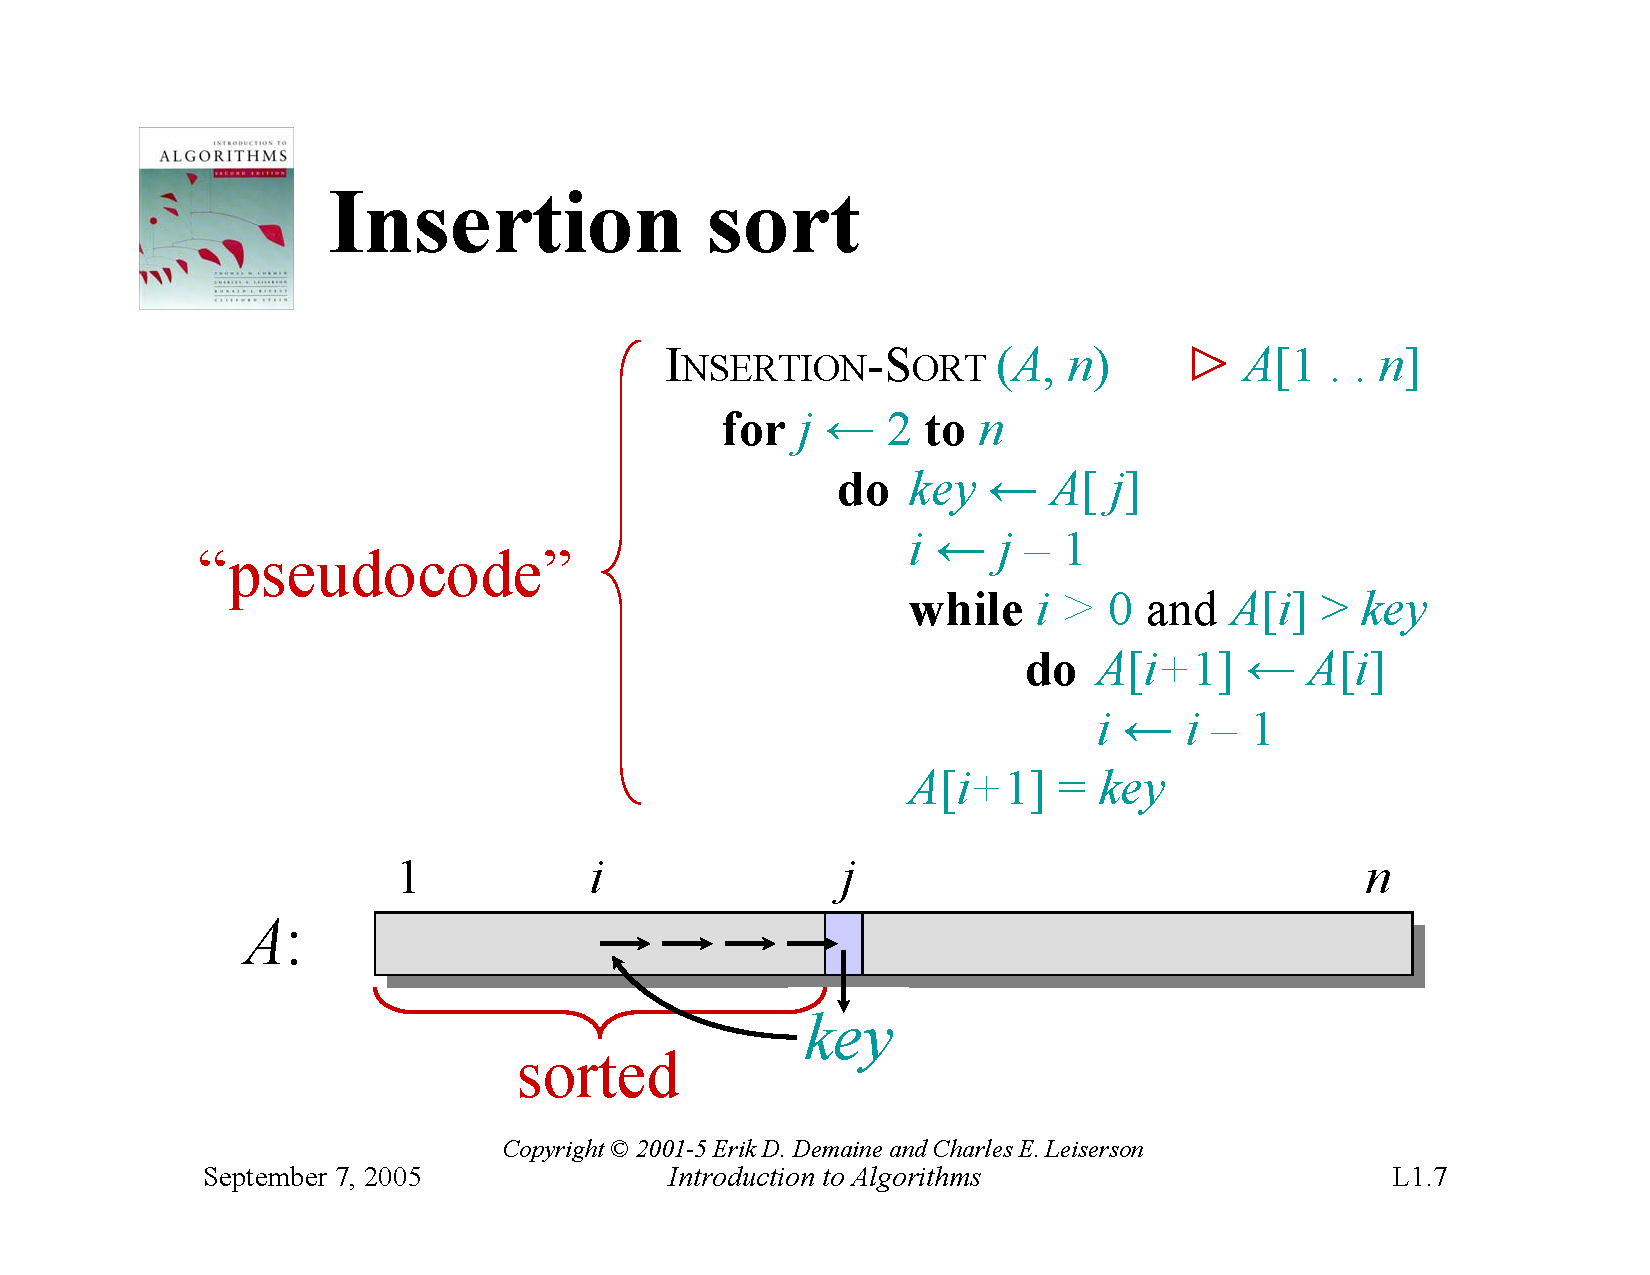
\includegraphics[width=\textwidth, trim={2cm 1cm 2cm 13cm}, clip]{pages/lec1_7}
\end{frame}

\begin{frame}{Example of insertion sort}
    \centering
    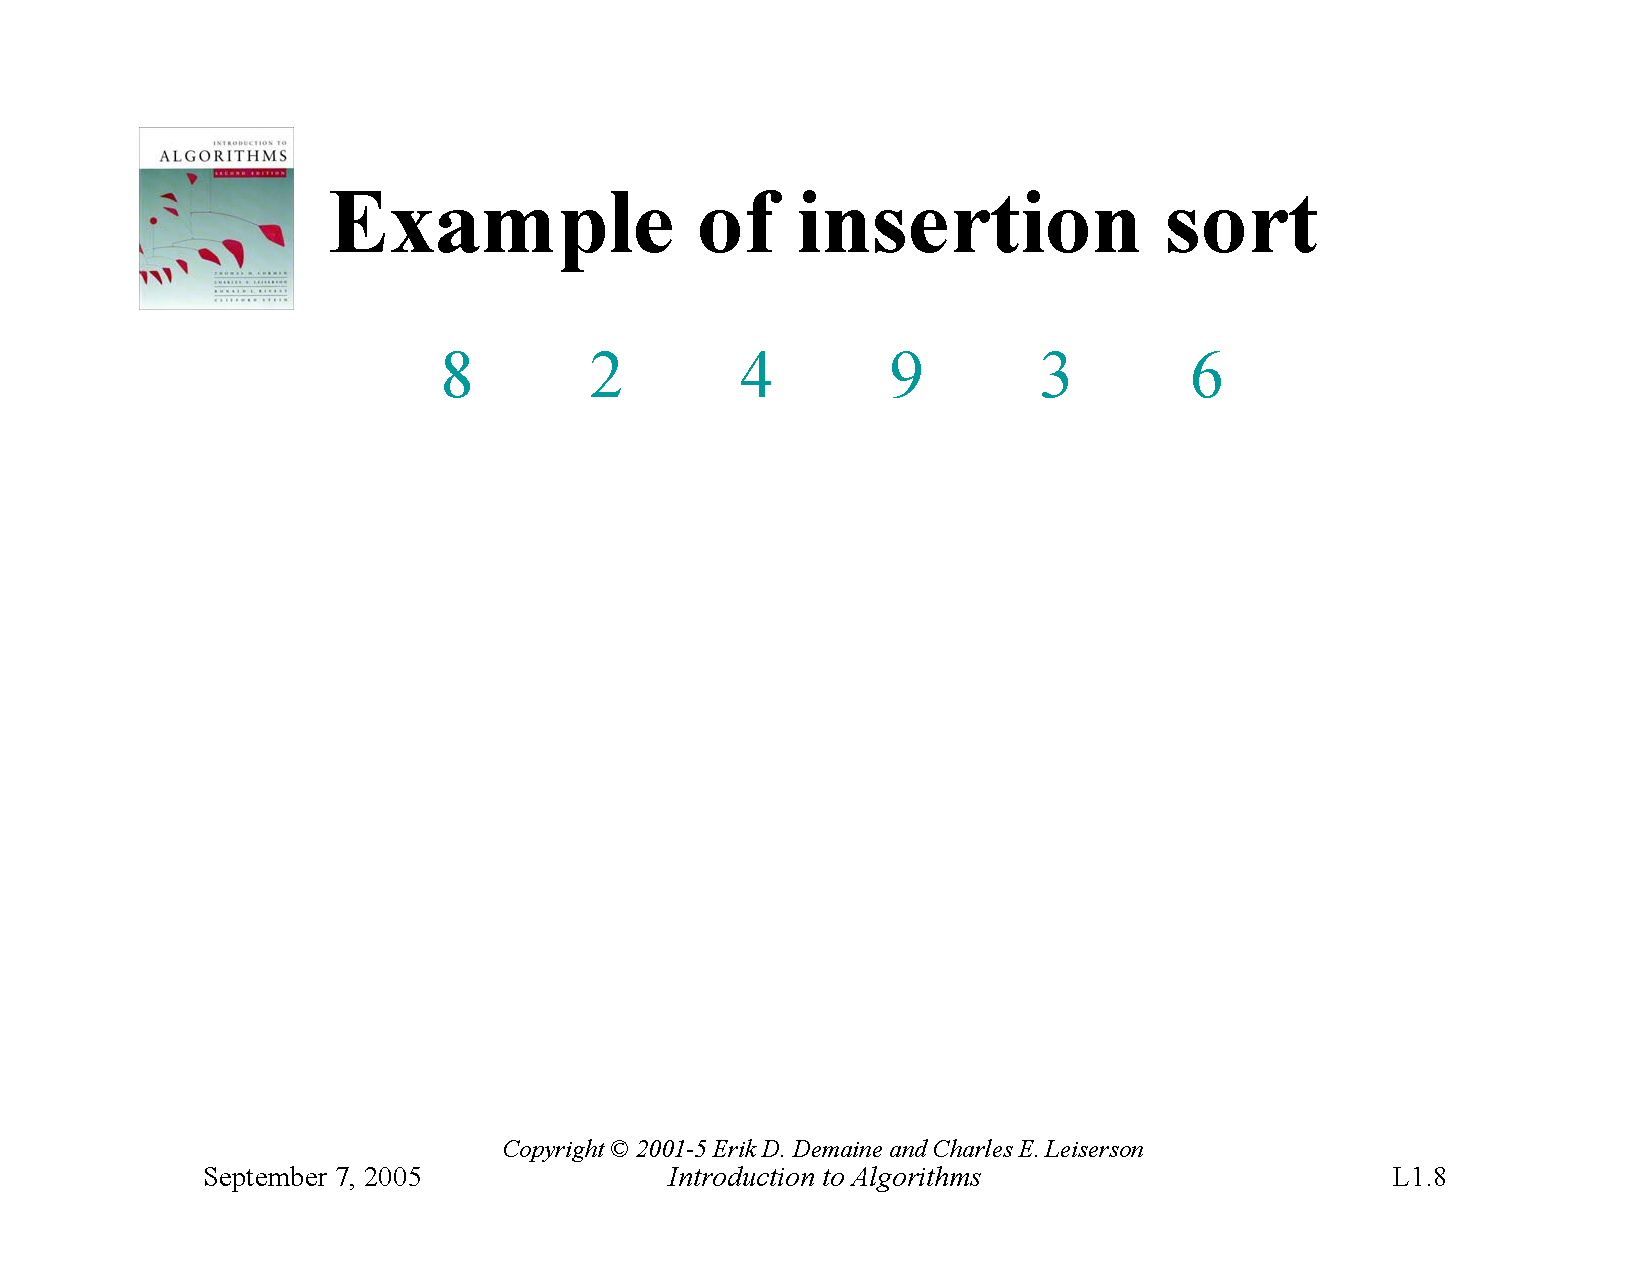
\includegraphics[width=0.9\textwidth, trim={5cm 2.95cm 5cm 4.25cm}, clip]{pages/lec1_8}
\end{frame}
\begin{frame}{Example of insertion sort}
    \centering
    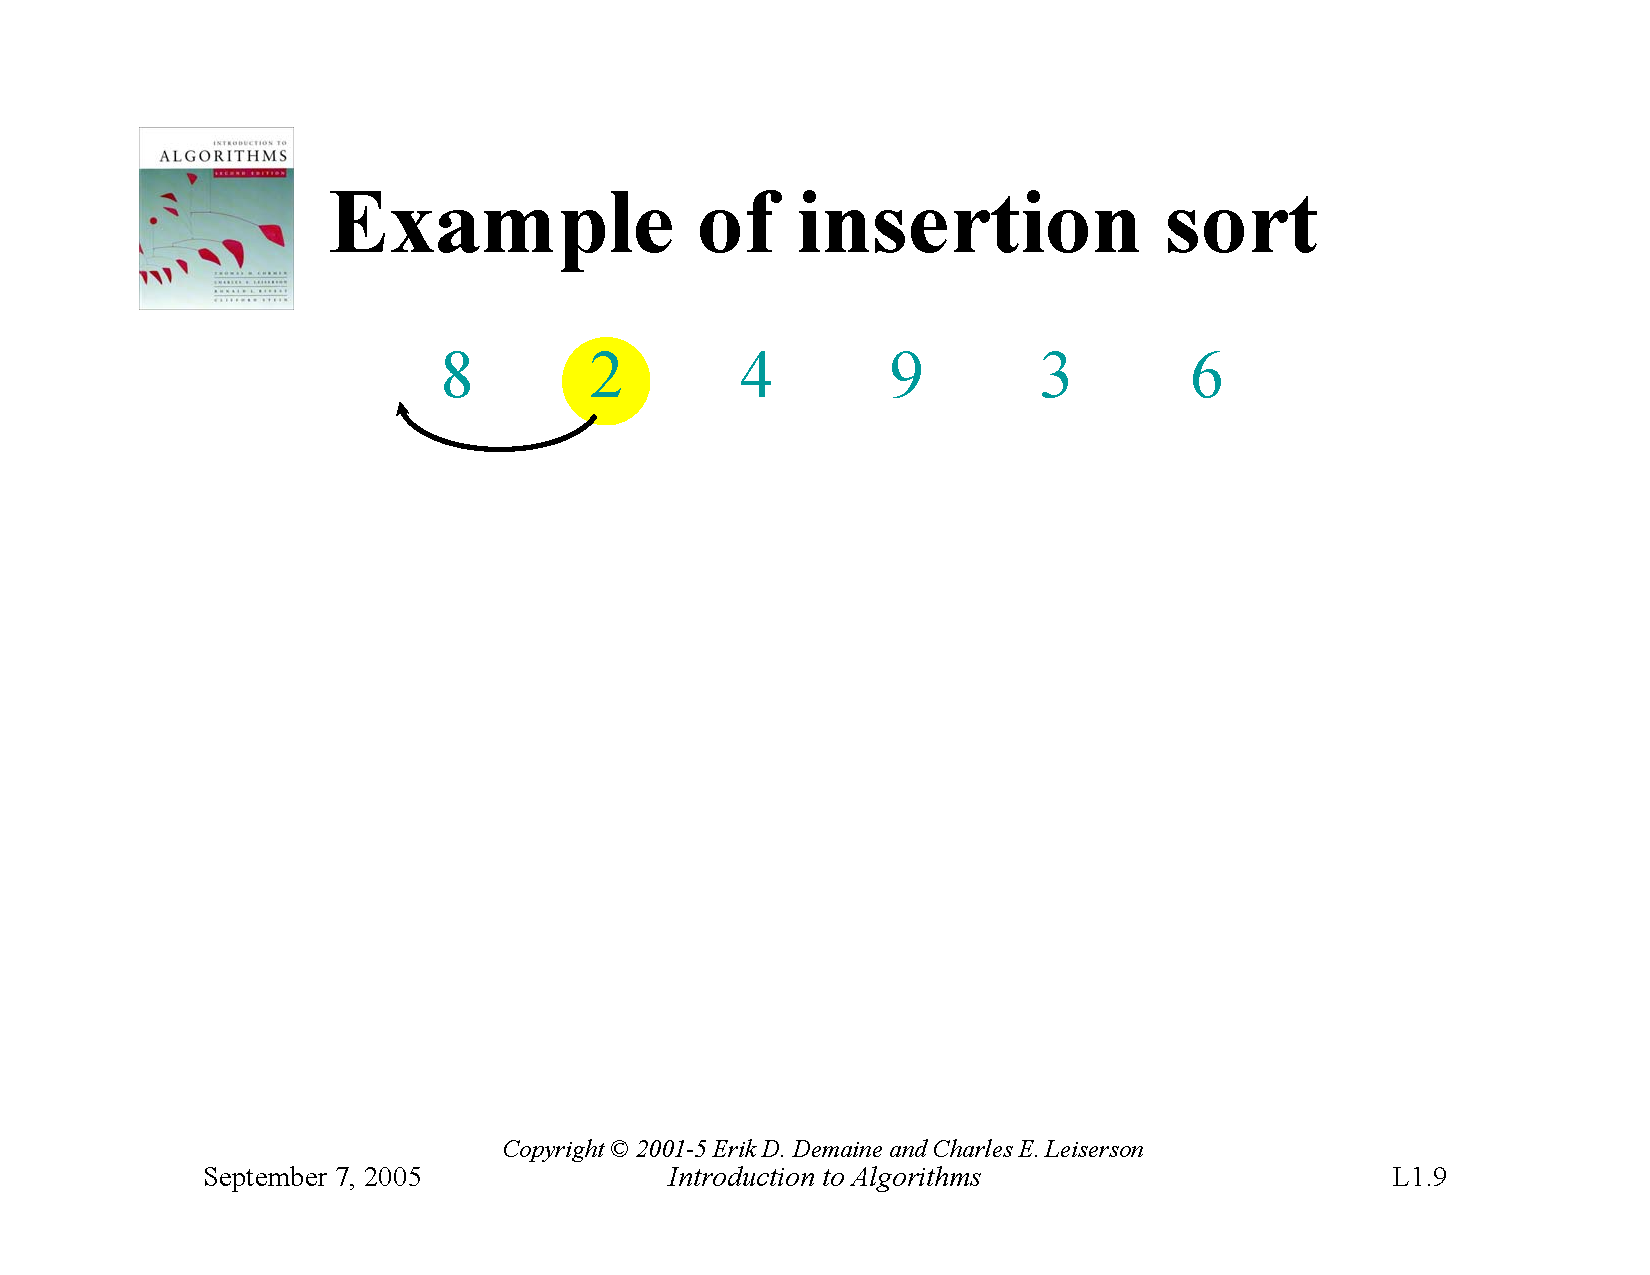
\includegraphics[width=0.9\textwidth, trim={5cm 2.95cm 5cm 4.25cm}, clip]{pages/lec1_9}
\end{frame}
\begin{frame}{Example of insertion sort}
    \centering
    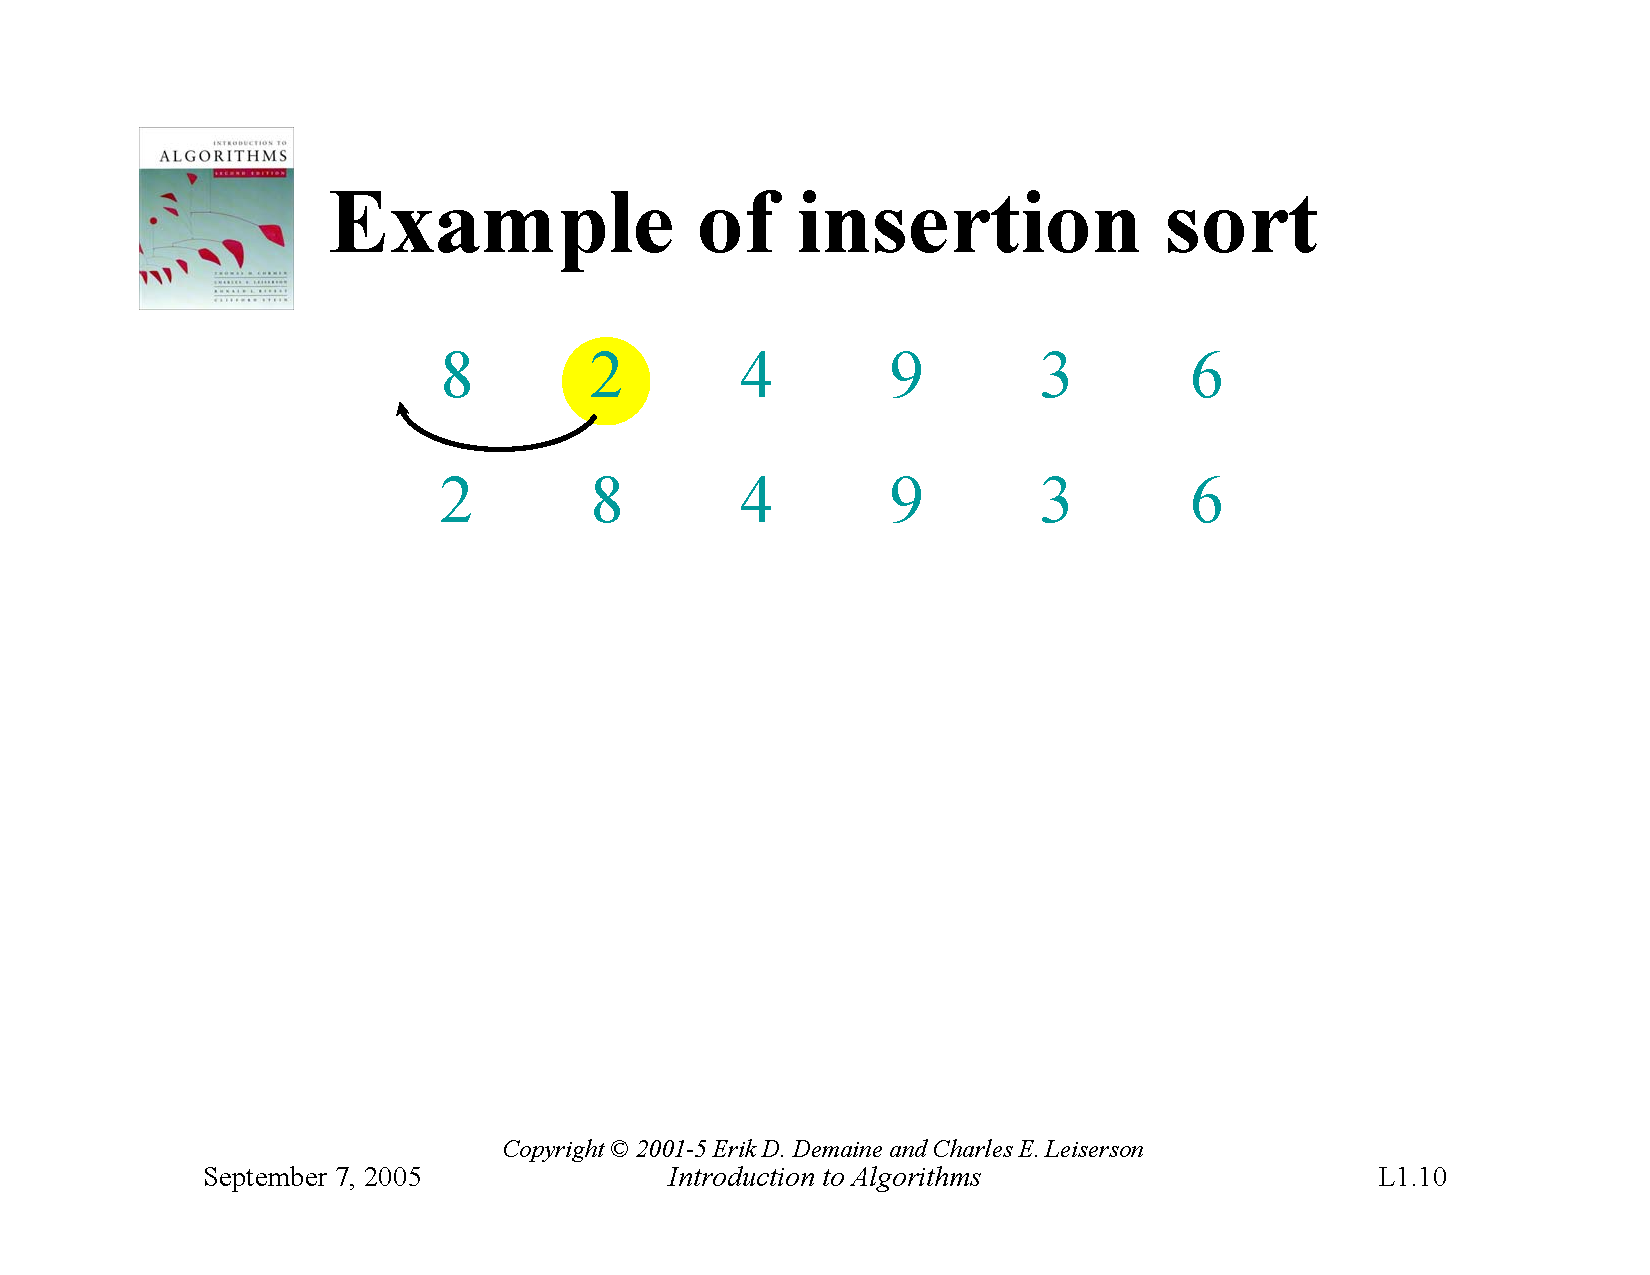
\includegraphics[width=0.9\textwidth, trim={5cm 2.95cm 5cm 4.25cm}, clip]{pages/lec1_10}
\end{frame}
\begin{frame}{Example of insertion sort}
    \centering
    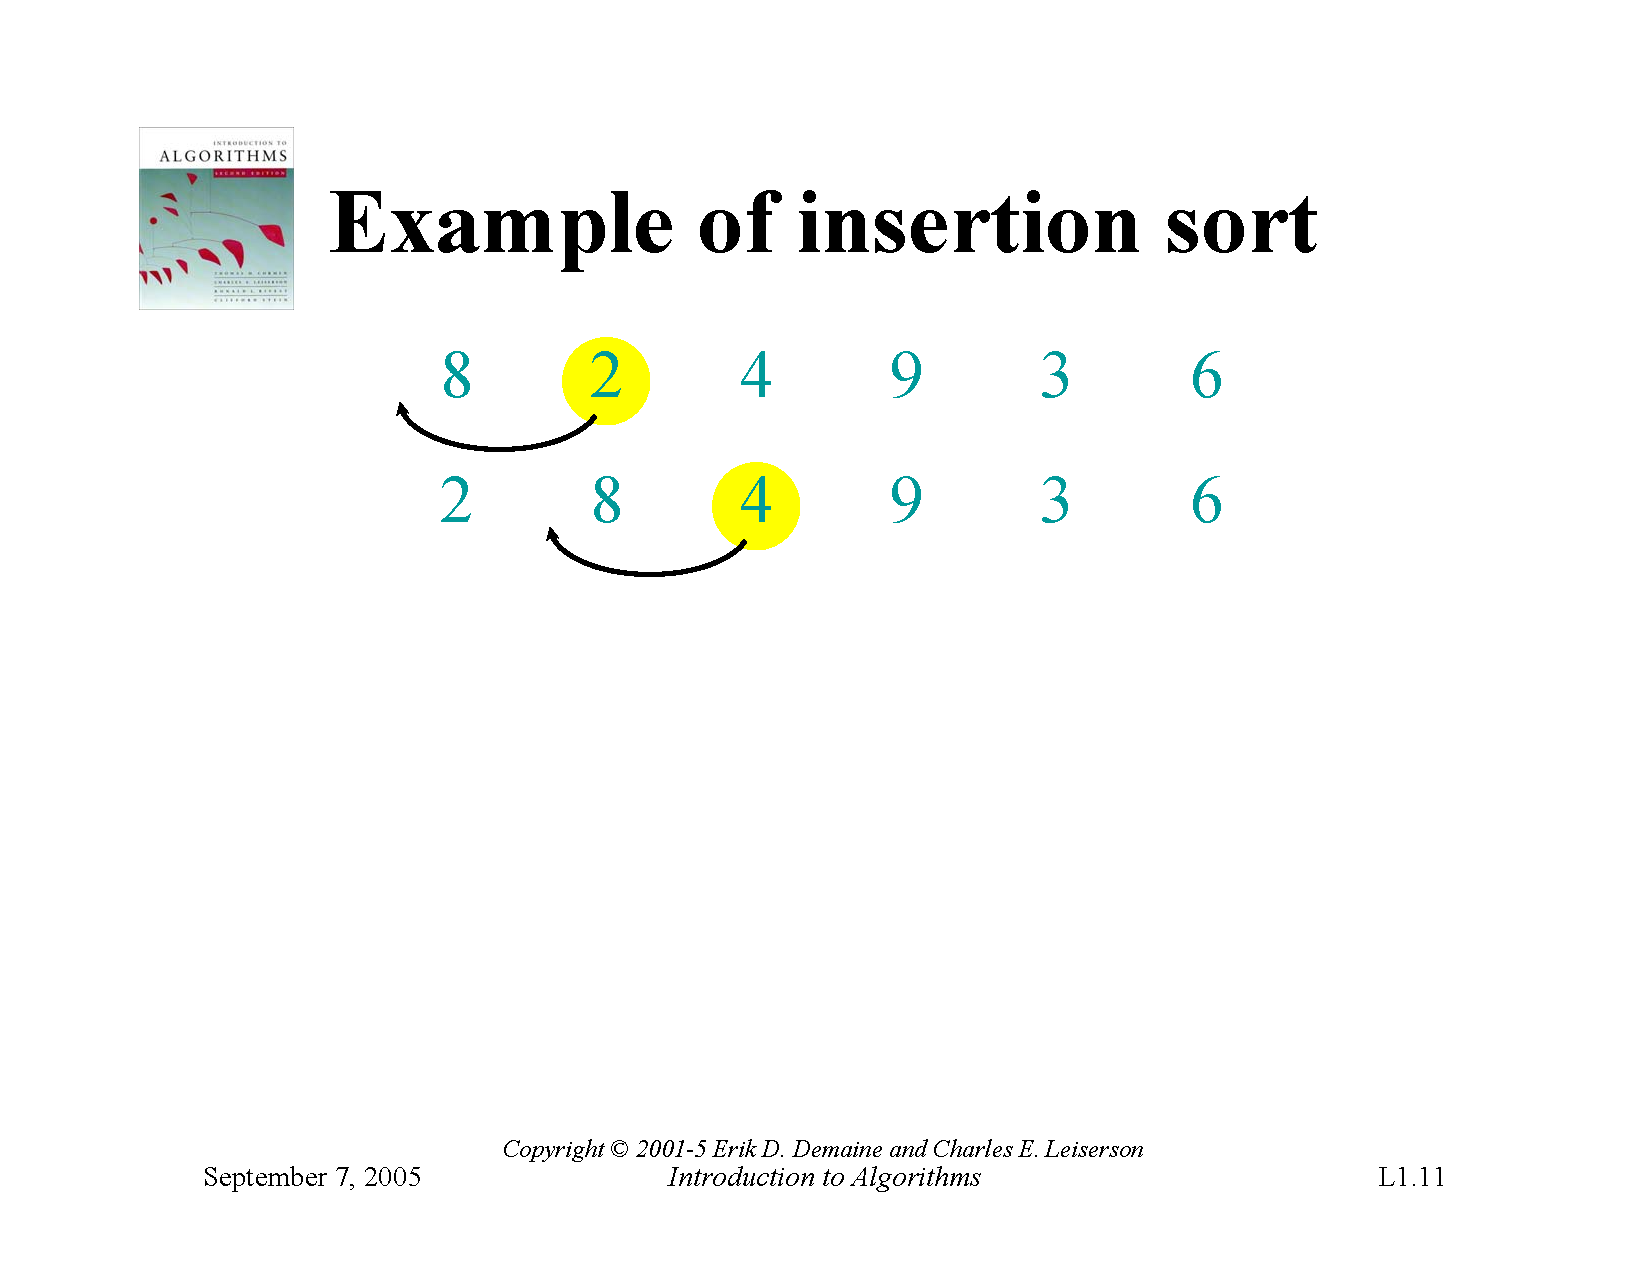
\includegraphics[width=0.9\textwidth, trim={5cm 2.95cm 5cm 4.25cm}, clip]{pages/lec1_11}
\end{frame}
\begin{frame}{Example of insertion sort}
    \centering
    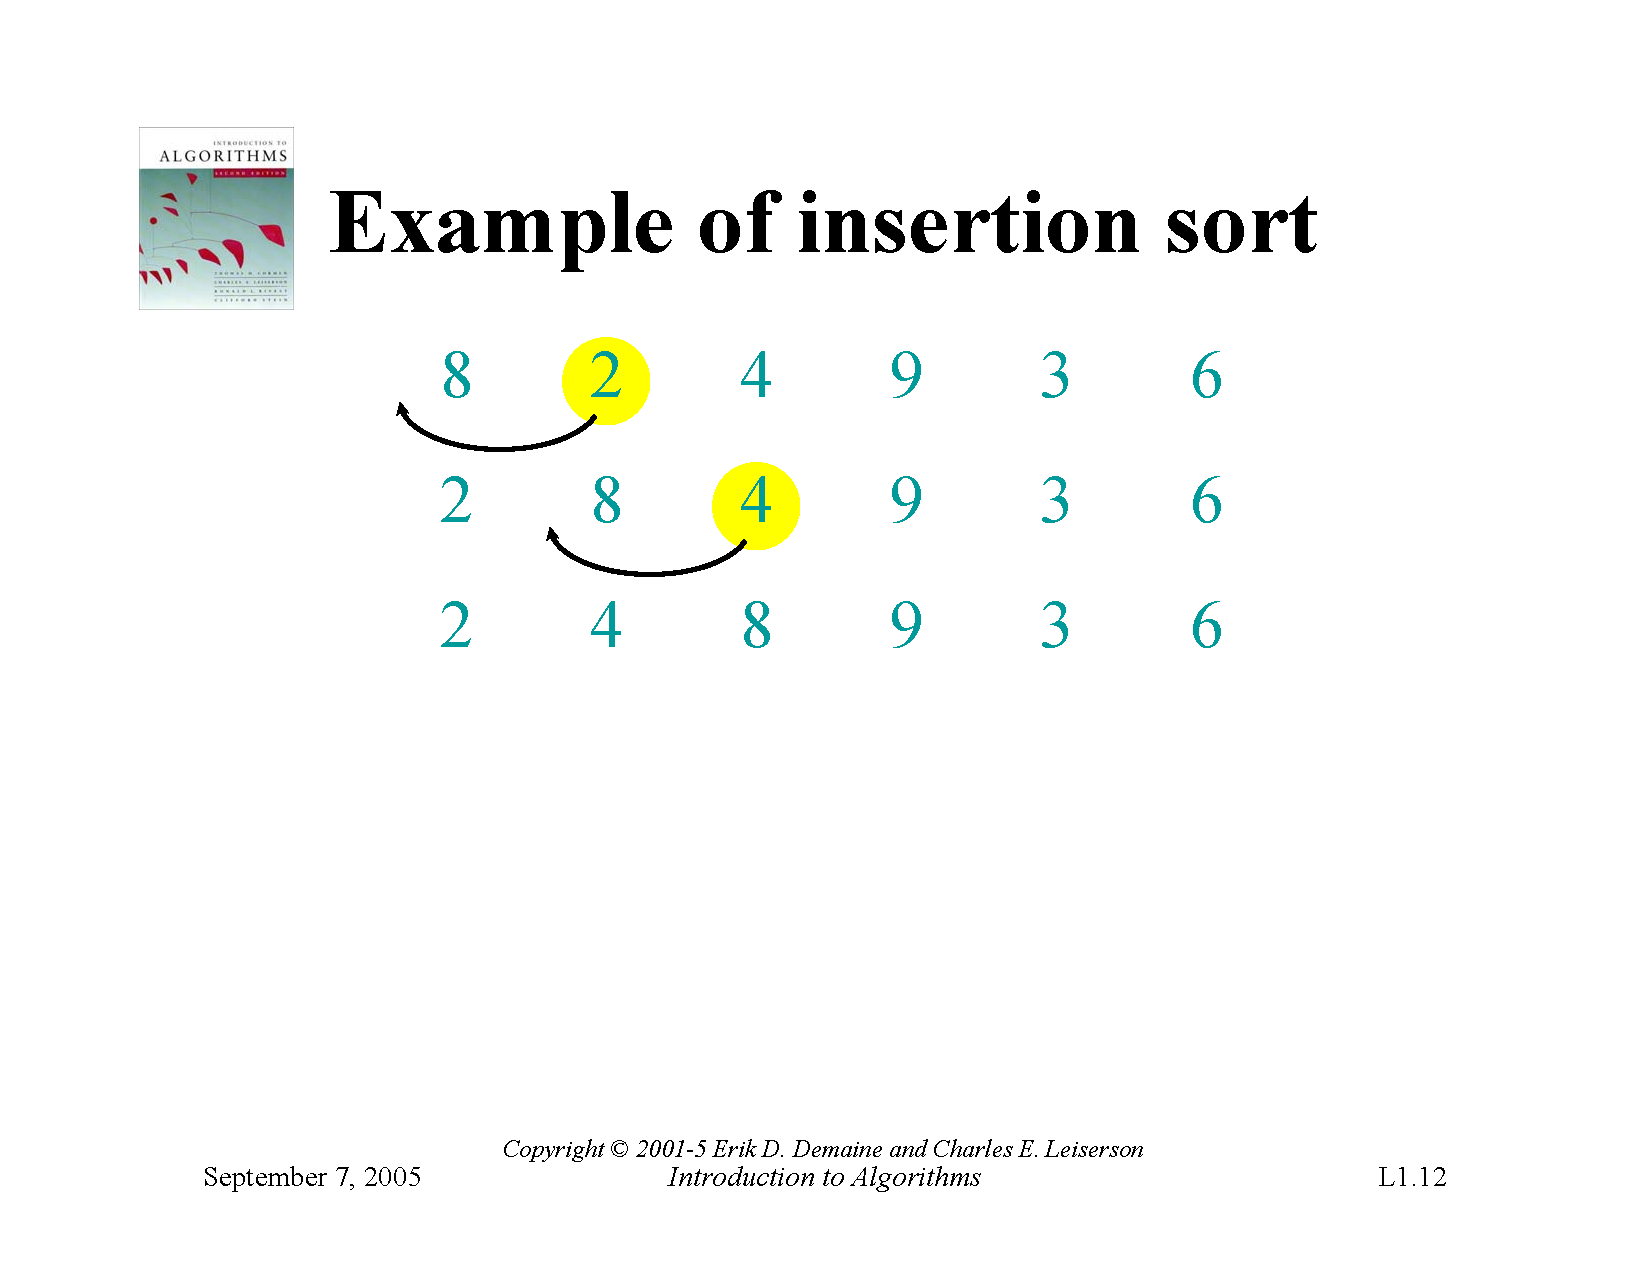
\includegraphics[width=0.9\textwidth, trim={5cm 2.95cm 5cm 4.25cm}, clip]{pages/lec1_12}
\end{frame}
\begin{frame}{Example of insertion sort}
    \centering
    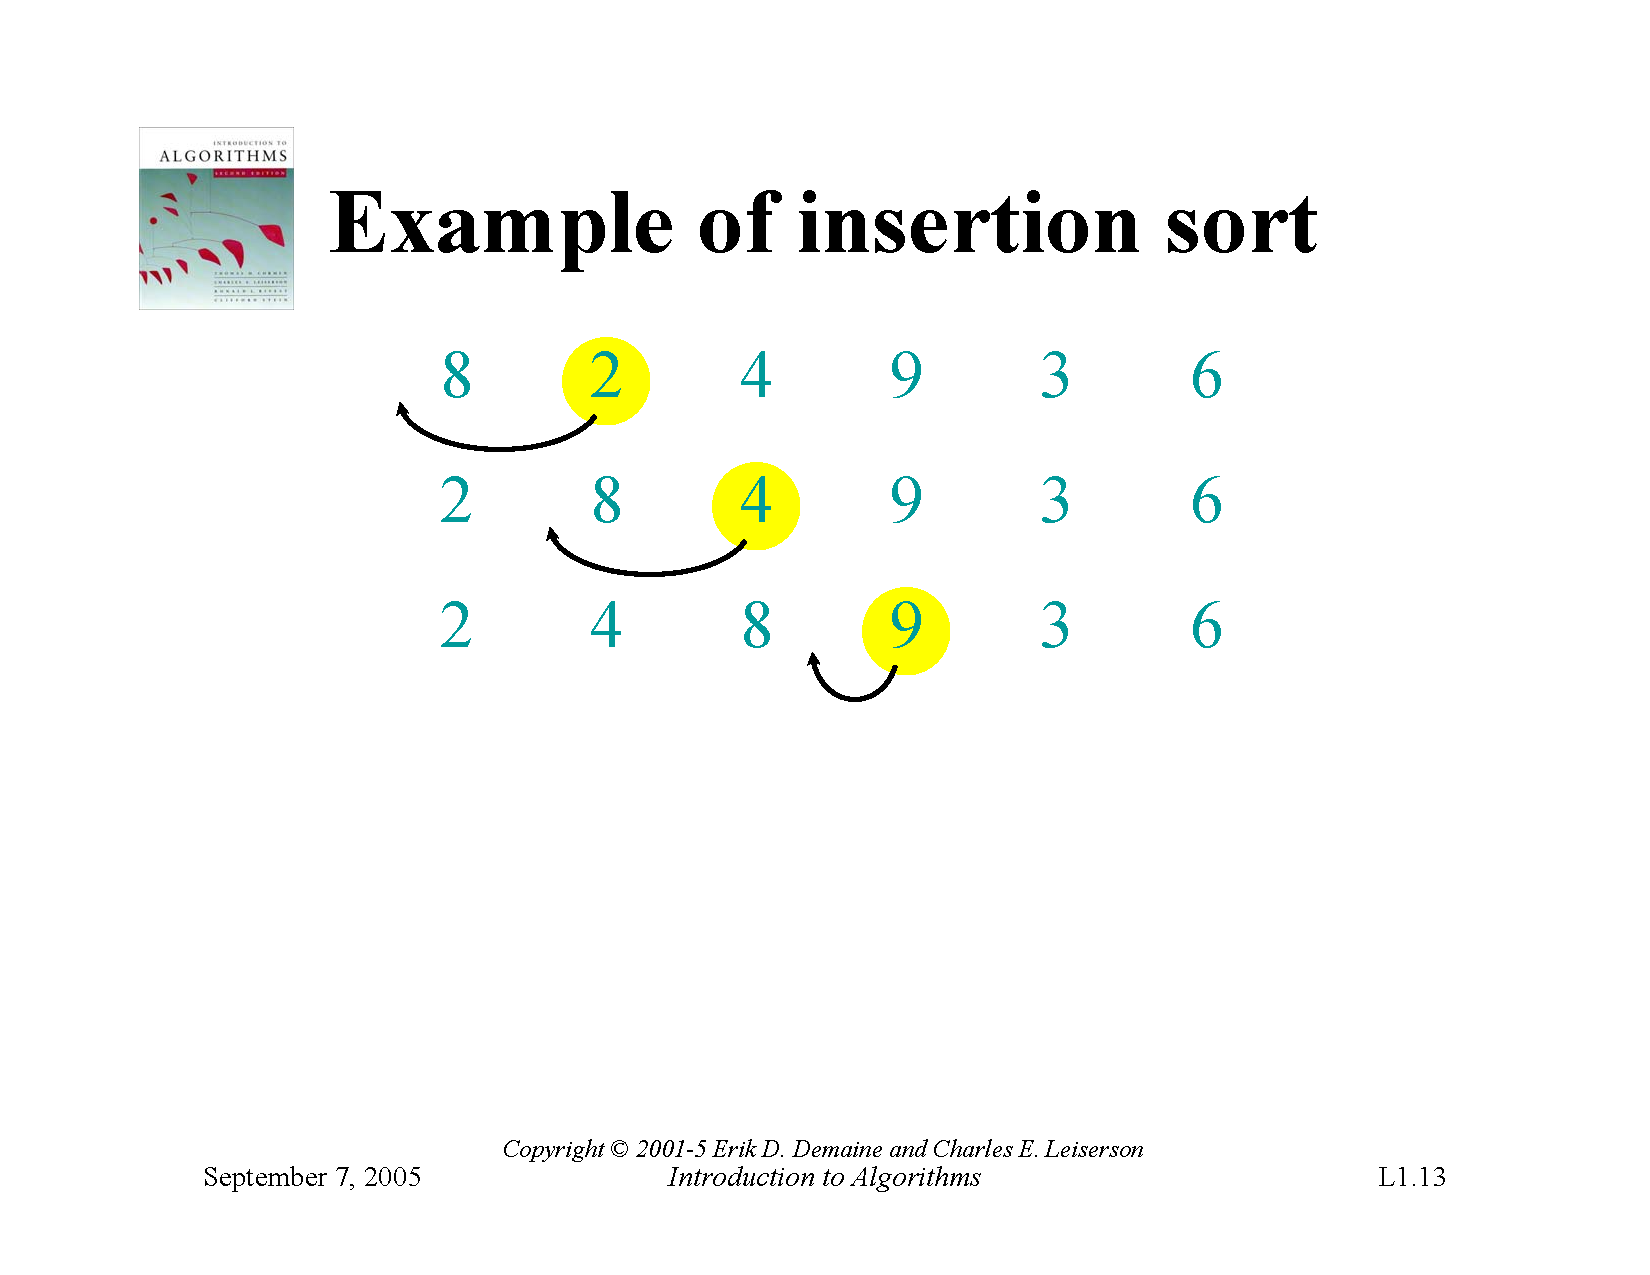
\includegraphics[width=0.9\textwidth, trim={5cm 2.95cm 5cm 4.25cm}, clip]{pages/lec1_13}
\end{frame}
\begin{frame}{Example of insertion sort}
    \centering
    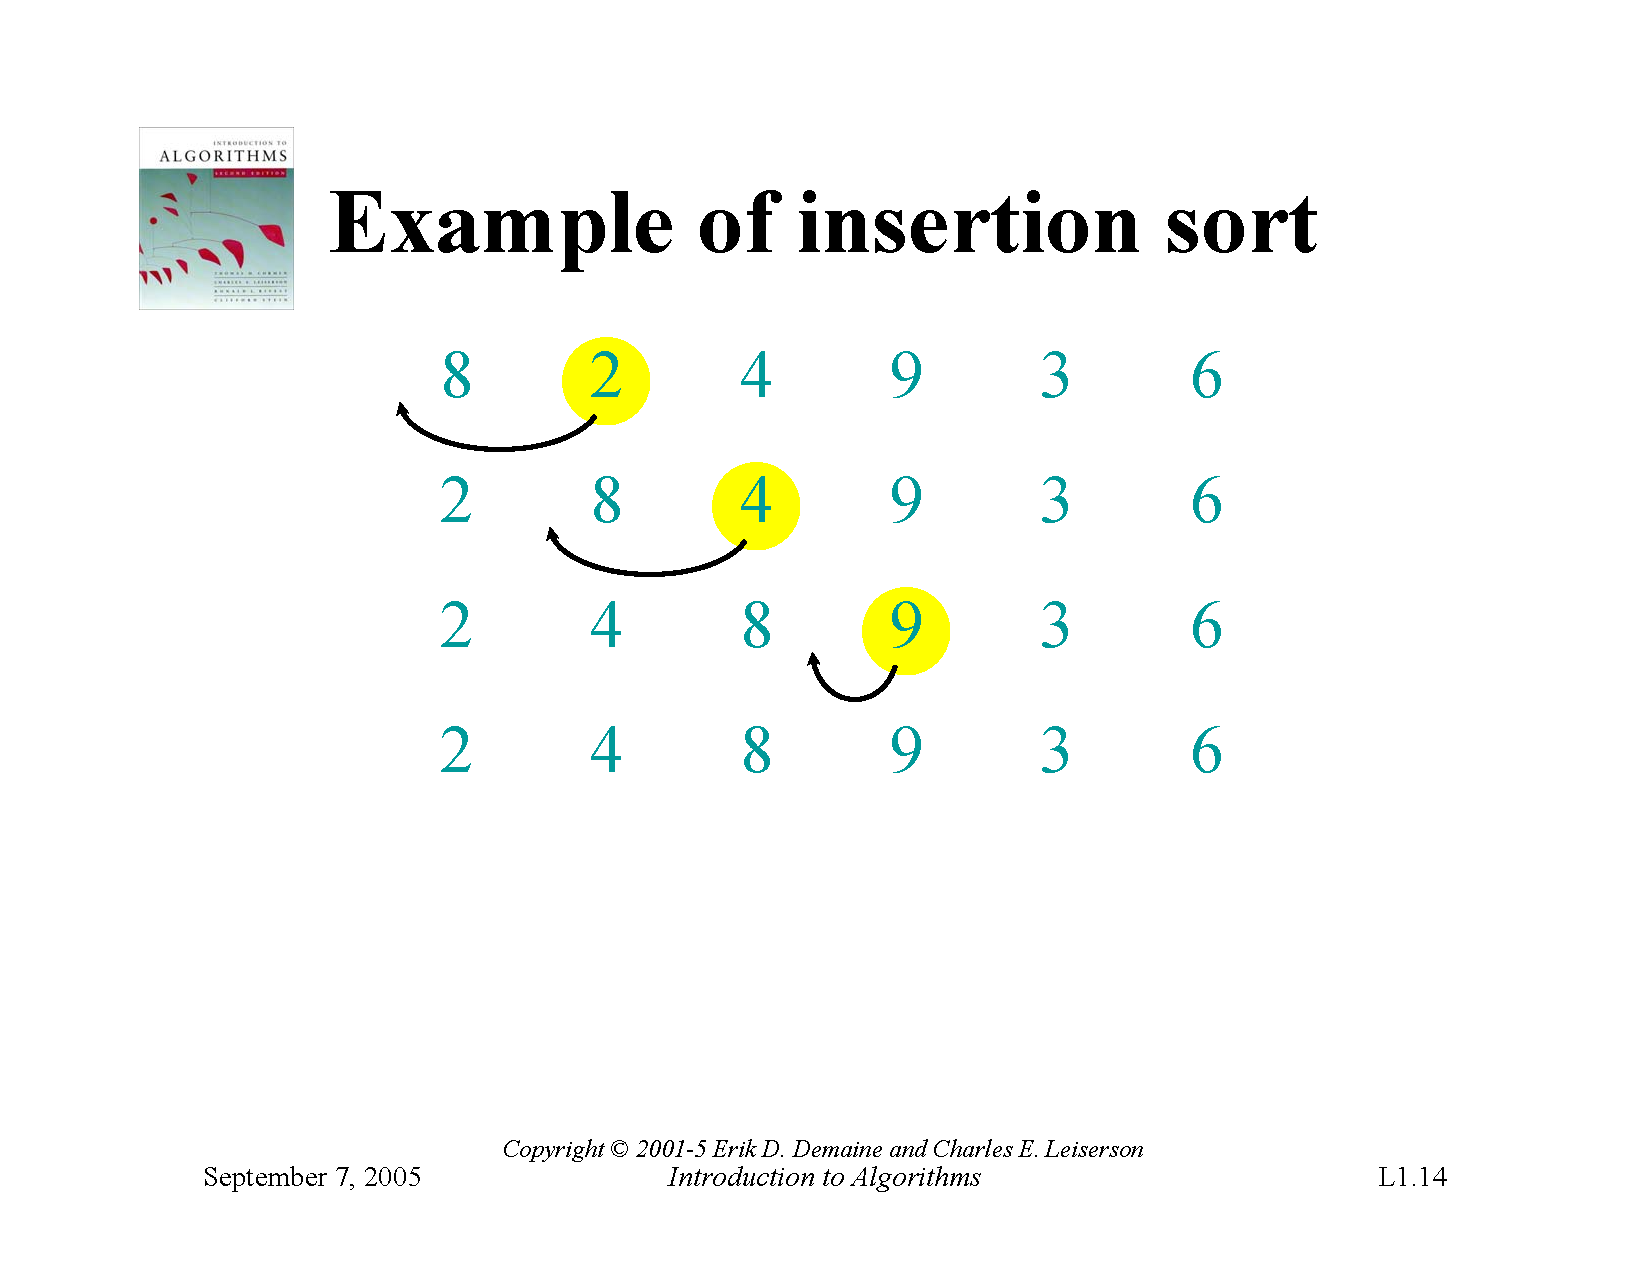
\includegraphics[width=0.9\textwidth, trim={5cm 2.95cm 5cm 4.25cm}, clip]{pages/lec1_14}
\end{frame}
\begin{frame}{Example of insertion sort}
    \centering
    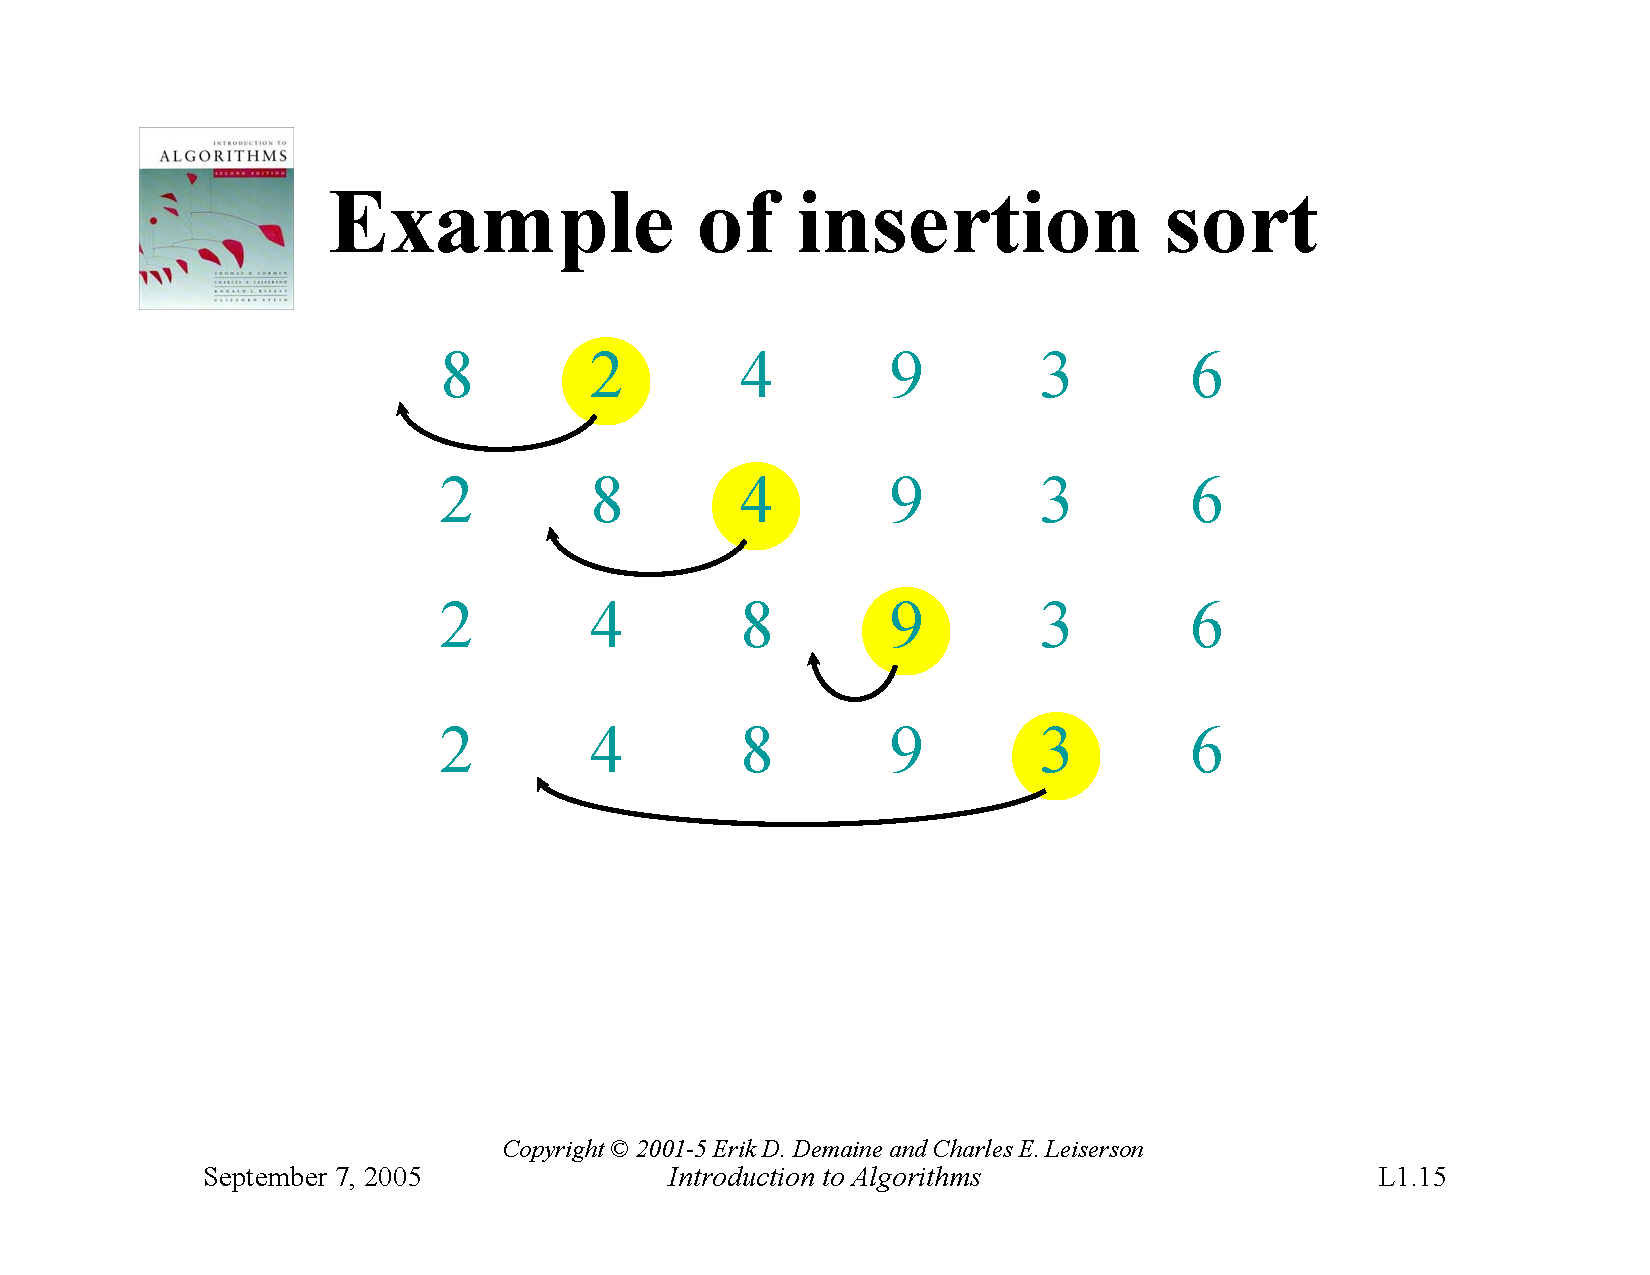
\includegraphics[width=0.9\textwidth, trim={5cm 2.95cm 5cm 4.25cm}, clip]{pages/lec1_15}
\end{frame}
\begin{frame}{Example of insertion sort}
    \centering
    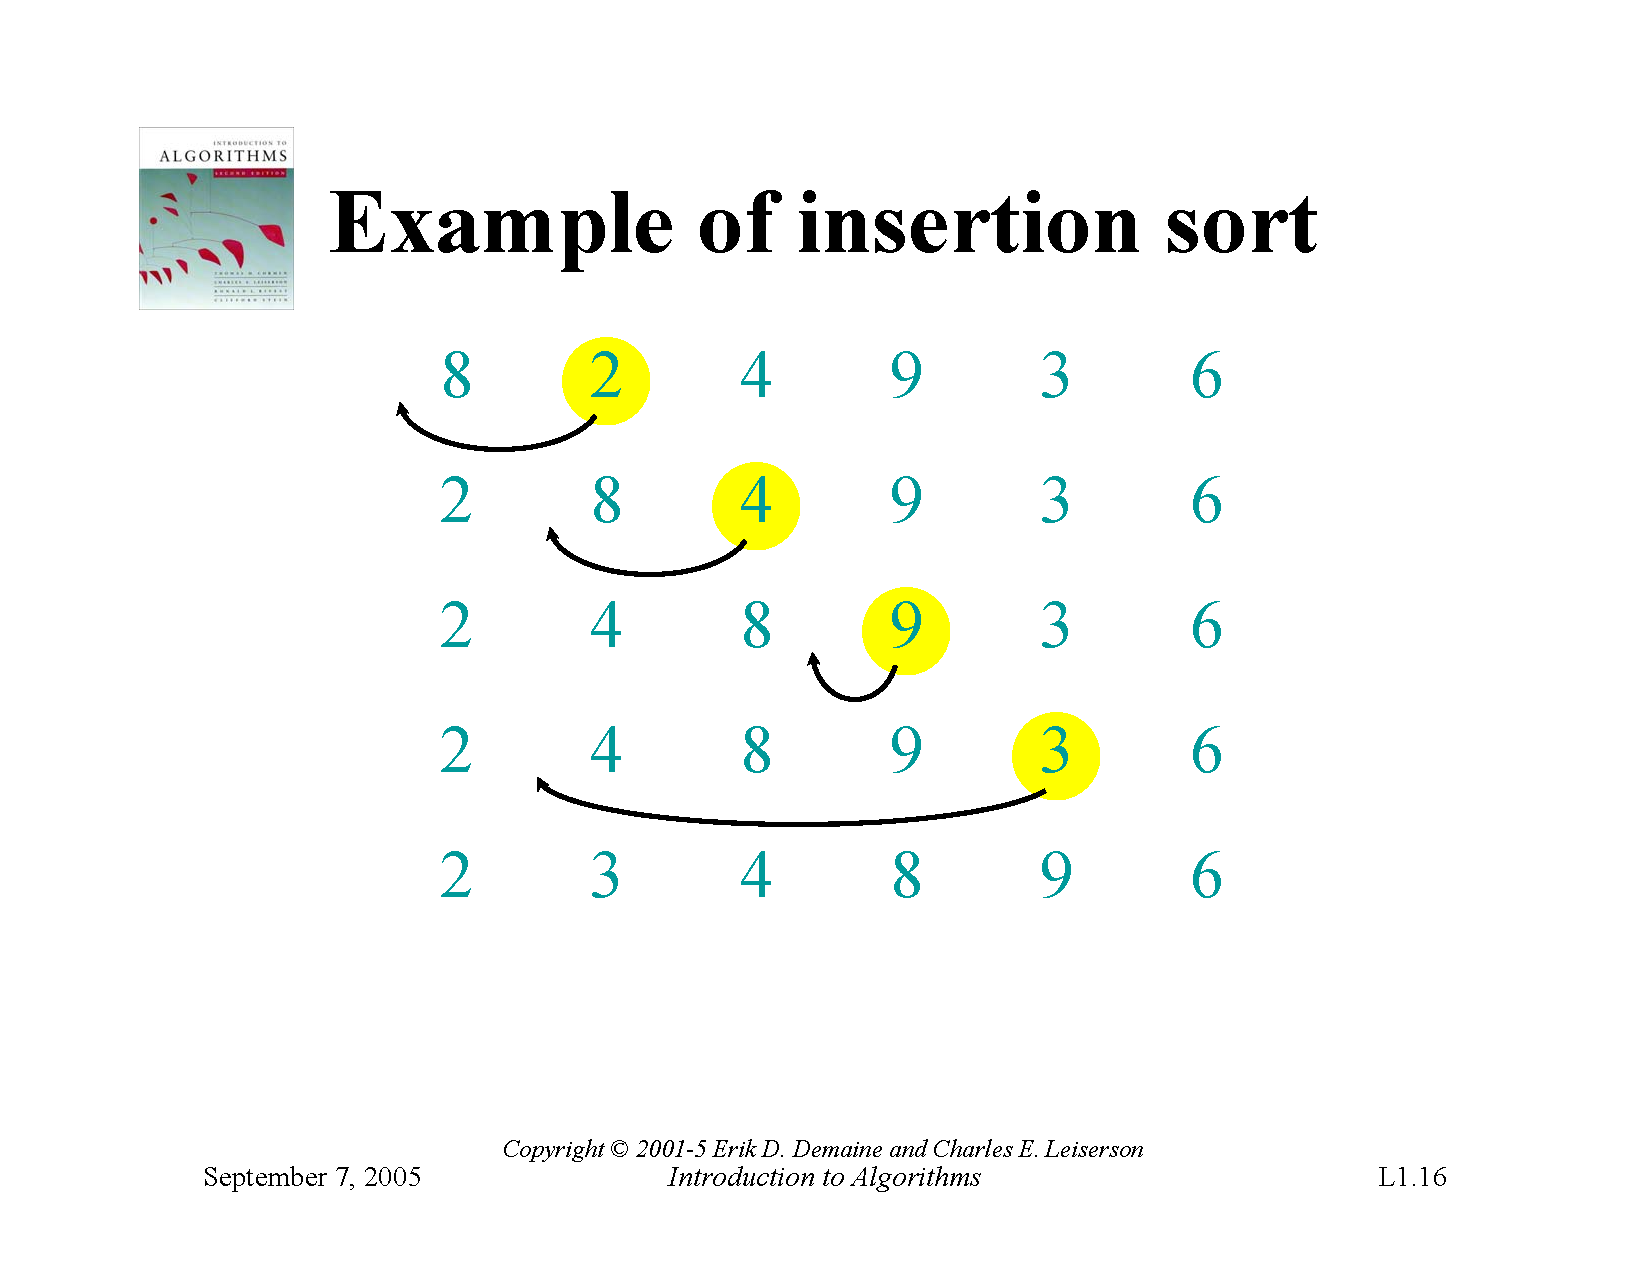
\includegraphics[width=0.9\textwidth, trim={5cm 2.95cm 5cm 4.25cm}, clip]{pages/lec1_16}
\end{frame}
\begin{frame}{Example of insertion sort}
    \centering
    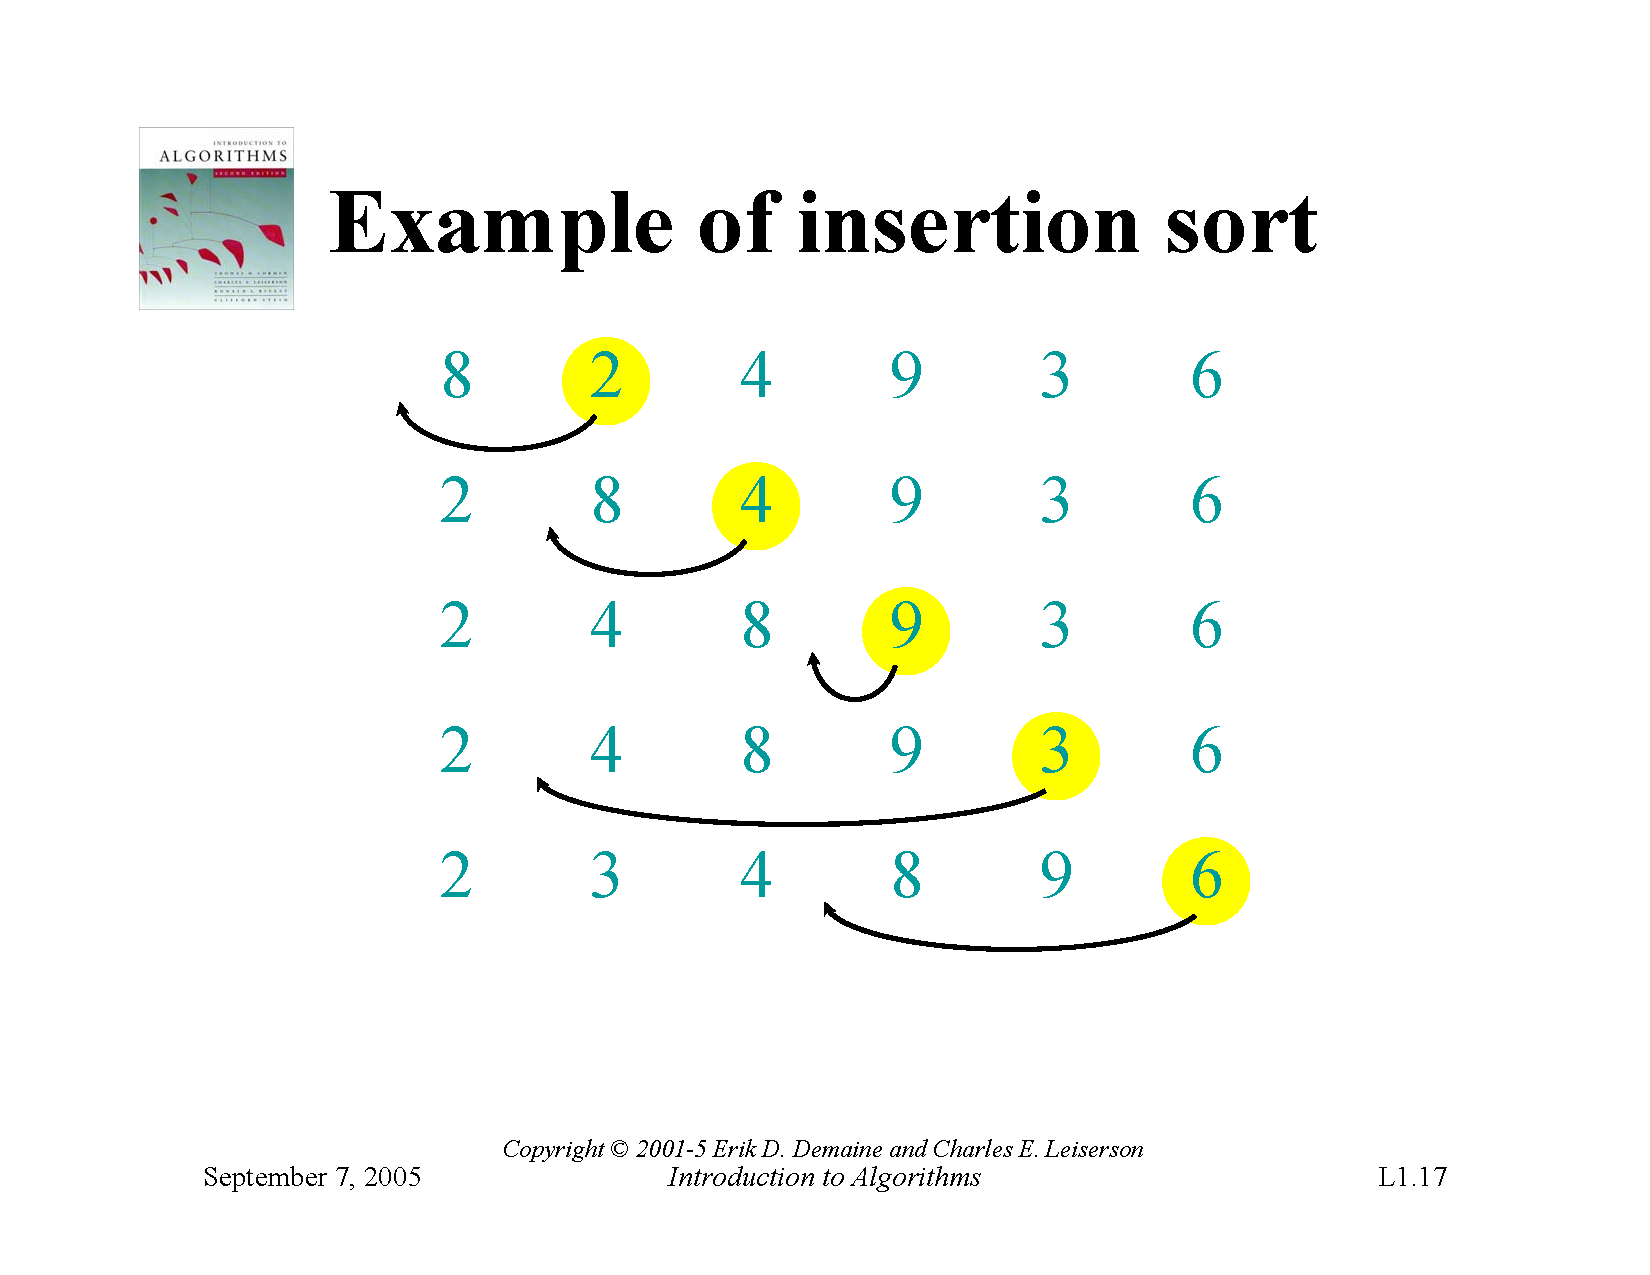
\includegraphics[width=0.9\textwidth, trim={5cm 2.95cm 5cm 4.25cm}, clip]{pages/lec1_17}
\end{frame}
\begin{frame}{Example of insertion sort}
    \centering
    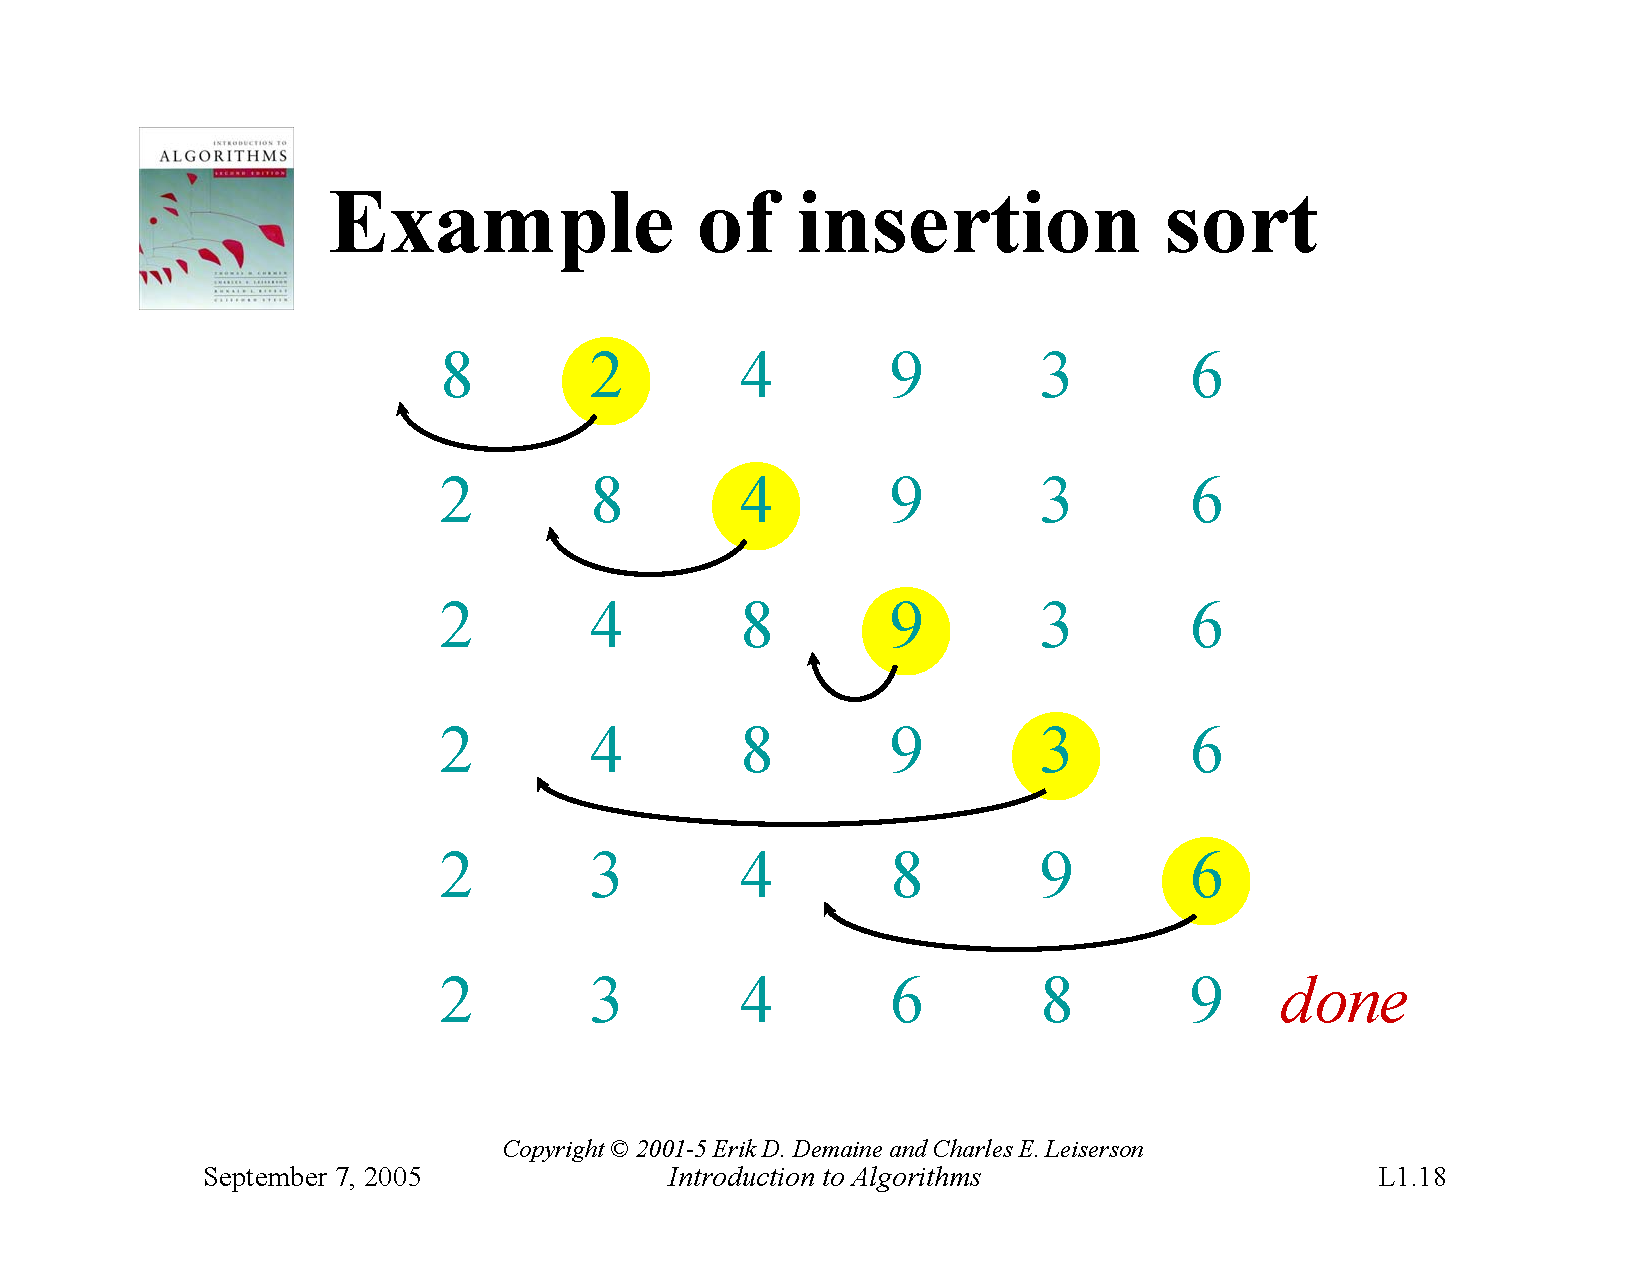
\includegraphics[width=0.9\textwidth, trim={5cm 2.95cm 5cm 4.25cm}, clip]{pages/lec1_18}
\end{frame}

\begin{frame}{Example of insertion sort}
    \centering
    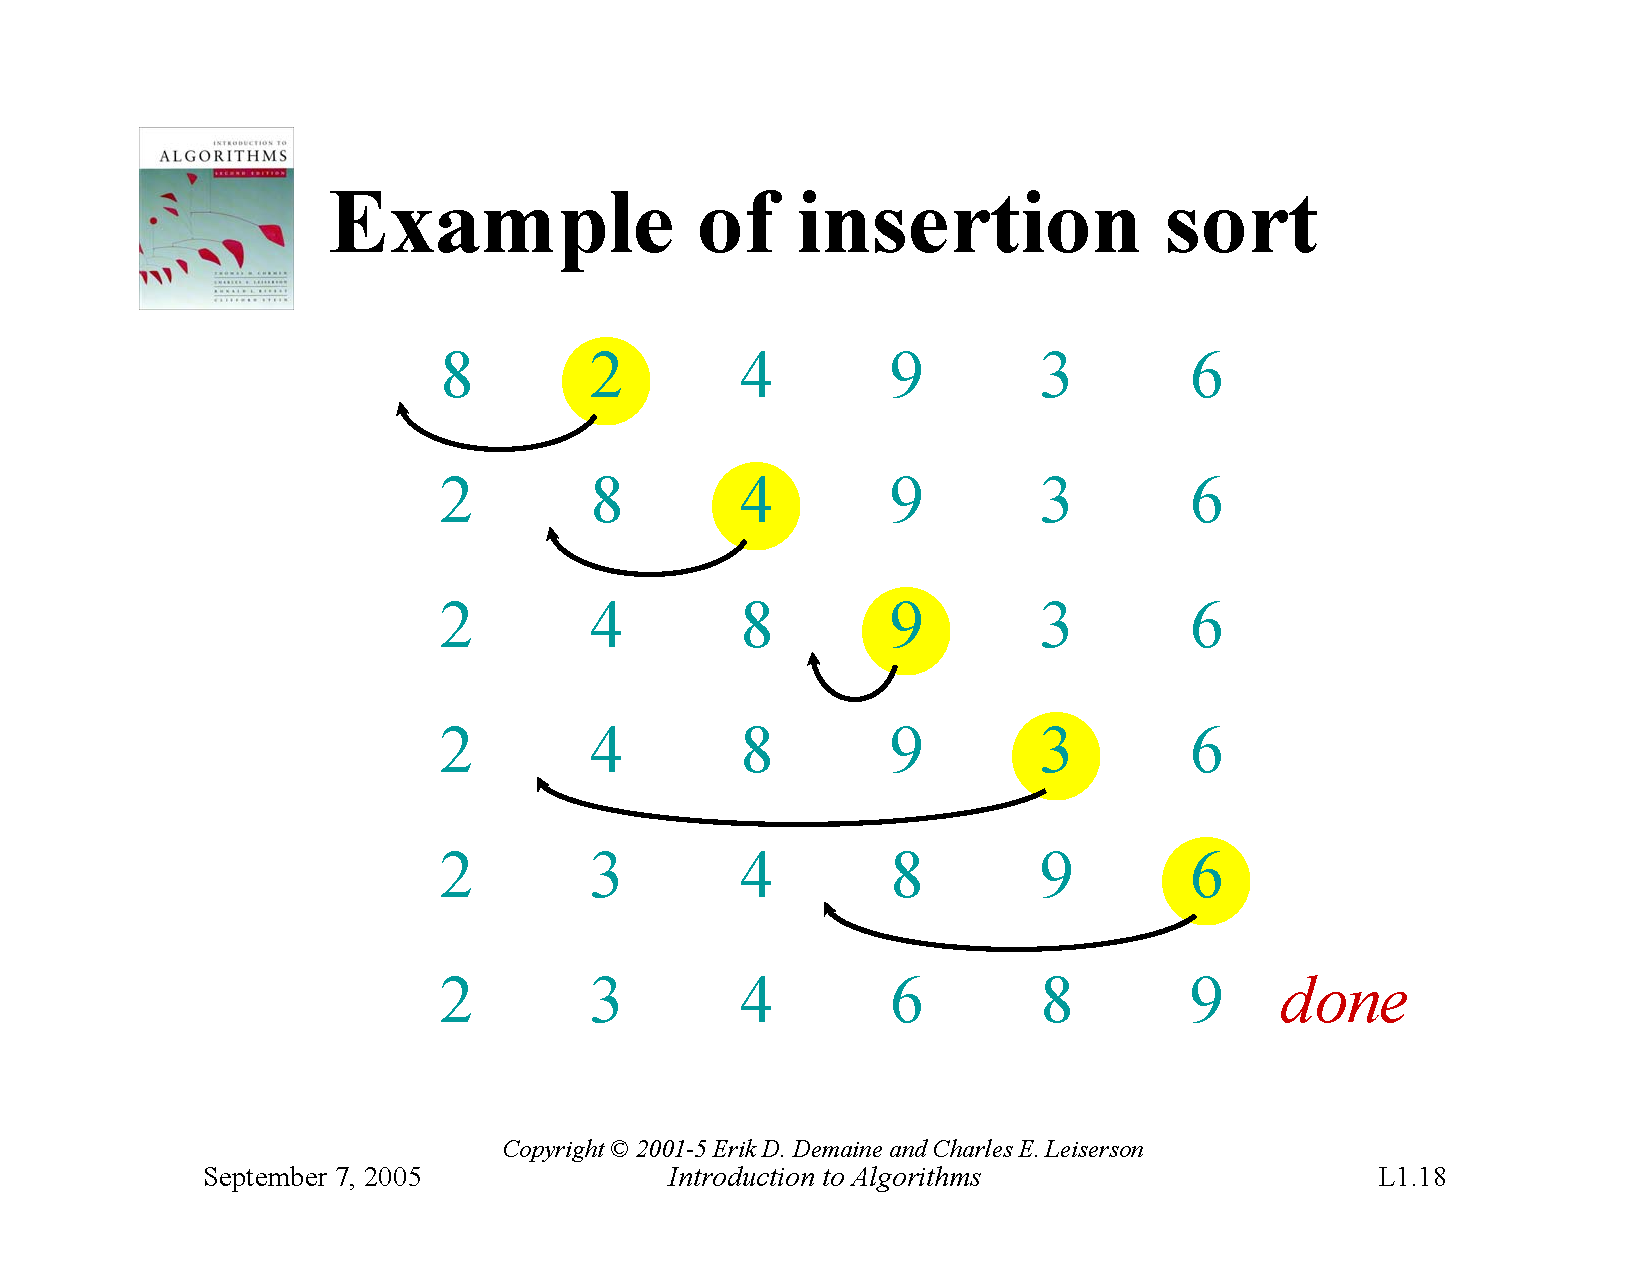
\includegraphics[width=0.9\textwidth, trim={5cm 2.95cm 5cm 4.25cm}, clip]{pages/lec1_18} \\
    \textbf{Done!}
\end{frame}

\begin{frame}{Running time}
    \begin{itemize}
        \item The running time depends on the input: an already sorted sequence is easier to sort.
        \item Parameterize the running time by the size of the input, since short sequences are easier to sort than long ones.
        \item Generally, we seek upper bounds on the running time, because everybody likes a guarantee.
    \end{itemize}
\end{frame}

\section{Asymptotic Analysis}

\begin{frame}{Kinds of analyses}
    \begin{itemize}
        \item Worst-case: (usually)
        \begin{itemize}
            \item $T(n)=$ \textit{maximum time} of algorithm on any input of size $n$.
        \end{itemize}
        \item Average-case: (sometimes)
        \begin{itemize}
            \item $T(n)=$ \textit{expected time} of algorithm over all inputs of size $n$.
            \item Need assumption of statistical distribution of inputs.
        \end{itemize}
        \item Best-case: (Bogus!)
        \begin{itemize}
            \item Cheat with a slow algorithm that works fast on \textit{some} input.
        \end{itemize}
    \end{itemize}
\end{frame}

\begin{frame}{Machine-independent time}
    ¿What is insertion sort's worst-case time?
    \begin{itemize}
        \item It depends on the speed of our computer:
        \begin{itemize}
            \item relative speed (on the same machine).
            \item absolute speed (on different machines).
        \end{itemize}
    \end{itemize}
    \textsc{Big Idea!}
    \begin{itemize}
     \item Ignore machine-dependent constants.
     \item Look at \textbf{growth} of $T(n)$ as $n \rightarrow \infty$
    \end{itemize}
    
    \centering
    \Large \textcolor{red}{``Asymptotic Analysis''}    
\end{frame}

\begin{frame}{$\Theta$-notation}
    \begin{itemize}
        \item Math:
        \begin{itemize}
            \item $\Theta(g(n)) = \{f(n):$ there exist positive constants $c_1$, $c_2$, and $n_0$ such that $0 \leq c_1g(n) \leq f(n) \leq c_2g(n)$ for all $n \geq n_0$
        \end{itemize}
        \item Engineering:
        \begin{itemize}
            \item Drop low-order terms; ignore leading constants.
            \item For instance: $3n^3+90n^2-5n+6046=\Theta(n^3)$
        \end{itemize}
    \end{itemize}
\end{frame}

\begin{frame}{Asymptotic Performance}
    When $n$ get large enough, a $\Theta(n^2)$ algorithm \textbf{always} beats a $\Theta(n^3)$ algorithm.\\
    \vspace{5mm}
    \begin{minipage}{0.5\textwidth}
        \centering
        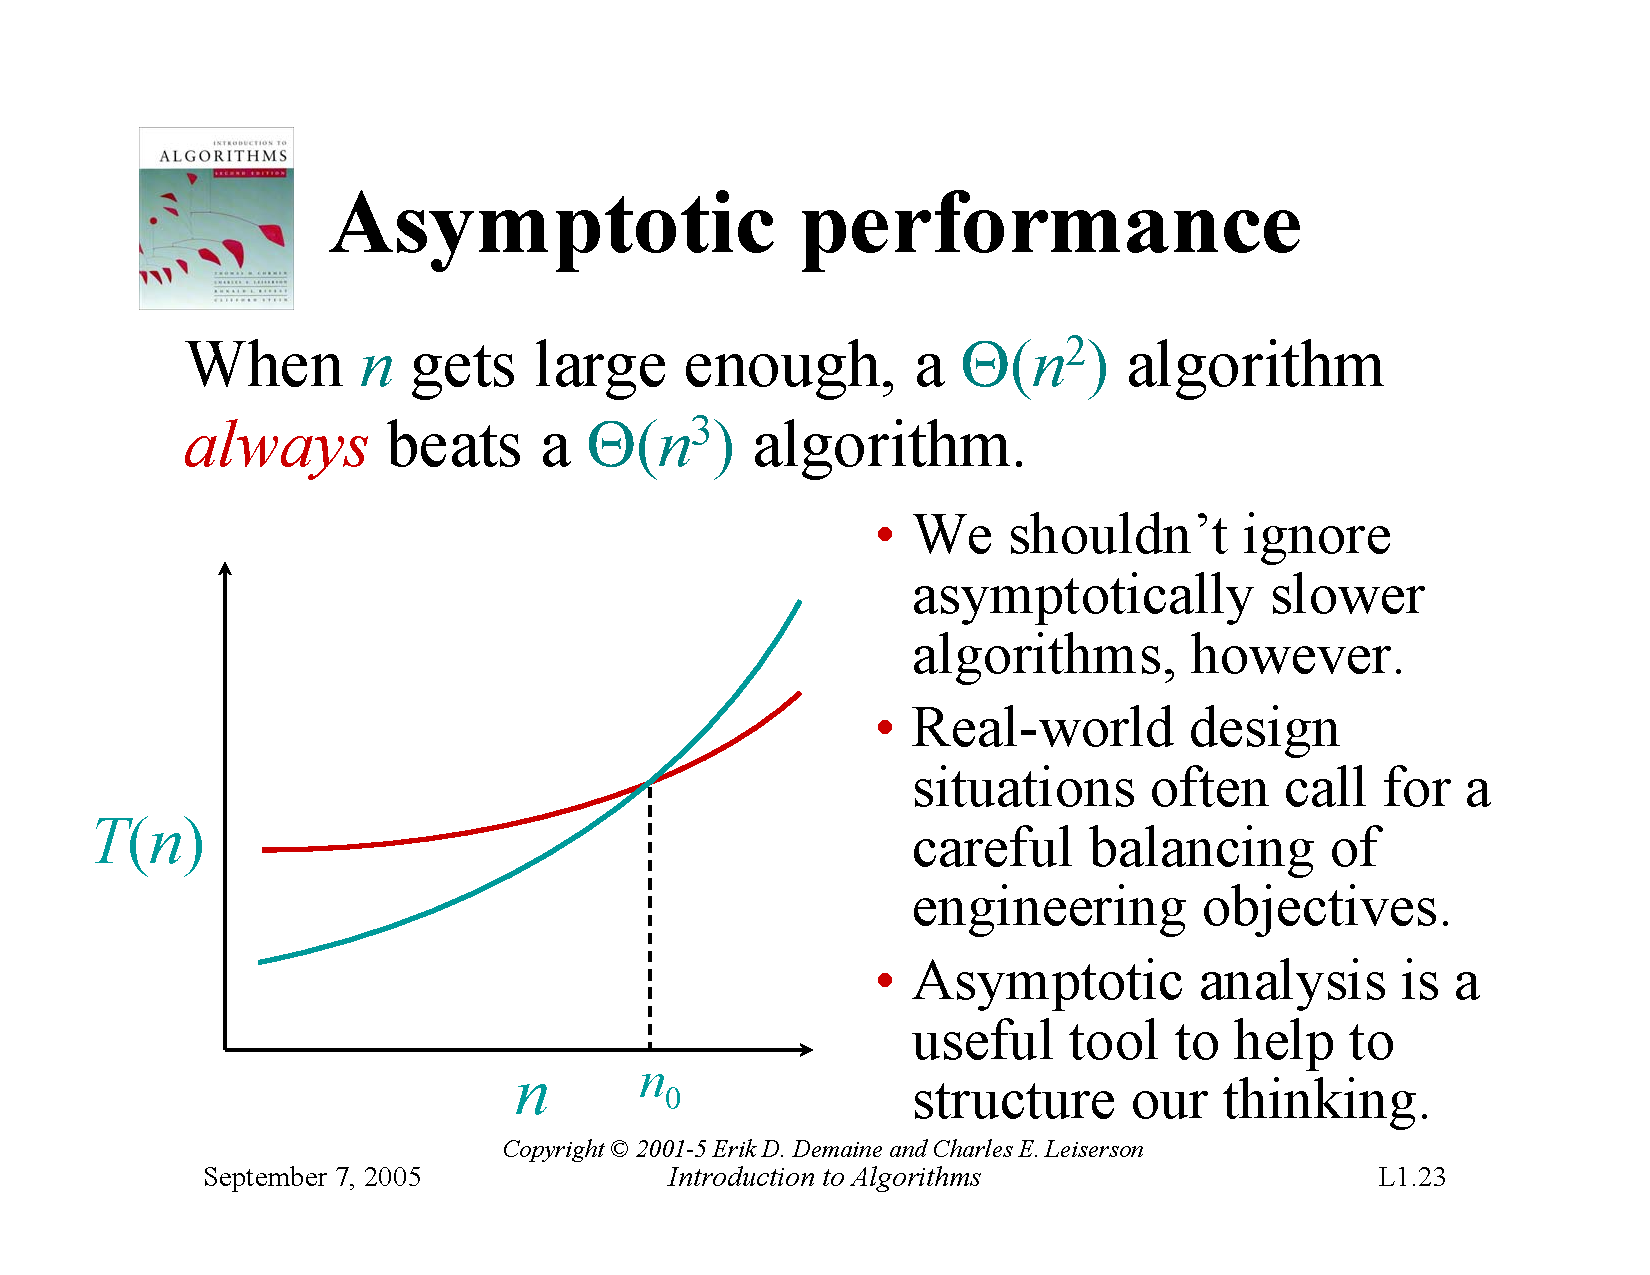
\includegraphics[width=\textwidth, trim={0.38cm 1.25cm 12.8cm 8.26cm}, clip]{pages/lec1_23} \\
    \end{minipage}
    \begin{minipage}{0.48\textwidth}
        \begin{itemize}
            \item We should not ignore asymptotically slower algorithms, however.
            \item Real-world design situations often call for a careful balancing of engineering objectives.
            \item Asymptotic analysis is a useful tool to help to structure our thinking.
        \end{itemize}
    \end{minipage}
\end{frame}

\begin{frame}{Insertion sort Analysis}
    \begin{itemize}
        \item \textbf{Worst case:} 
        \begin{itemize}
            \item Input reverse sorted.
            \item $T(n) = \sum^{n}_{j = 2} \Theta(j) = \Theta(n^2)$.
            \item Arithmetic series!
        \end{itemize}
        \item \textbf{Average case:}
        \begin{itemize}
            \item All permutations equally likely.
            \item $T(n) = \sum^{n}_{j = 2} \Theta(\frac{j}{2}) = \Theta(n^2)$.
        \end{itemize}
    \end{itemize}
    \begin{itemize}
        \item \textit{¿Is insertion sort a fast sorting algorithm?}
        \begin{itemize}
            \item Moderately so, for small $n$.
            \item Not at all, for large $n$.
        \end{itemize}

    \end{itemize}

\end{frame}

\section{Merge-sort}

\begin{frame}{Merge-sort}
    \begin{algorithm}[H]
        \caption{Insertion Sort}
        \begin{algorithmic}[1]
            \STATE \textsc{Merge-sort}$(A, n)$ \hspace{5mm} $\rhd A[1 \ldots n]$ 
            \STATE \hspace{1em} \textbf{if} $n = 1$, done.
            \STATE \hspace{1em} Recursively sort $A[ 1 \ldots \lceil \frac{n}{2} \rceil ]$ and $A[ \lceil \frac{n}{2} \rceil + 1 \ldots n ]$
            \STATE \hspace{1em} \textsc{Merge} the 2 sorted list.
        \end{algorithmic}
    \end{algorithm}
    \vspace{5mm}
    \centering
    Key subroutine: \textsc{Merge}
\end{frame}

\begin{frame}{Merging two sorted arrays}
    \centering
    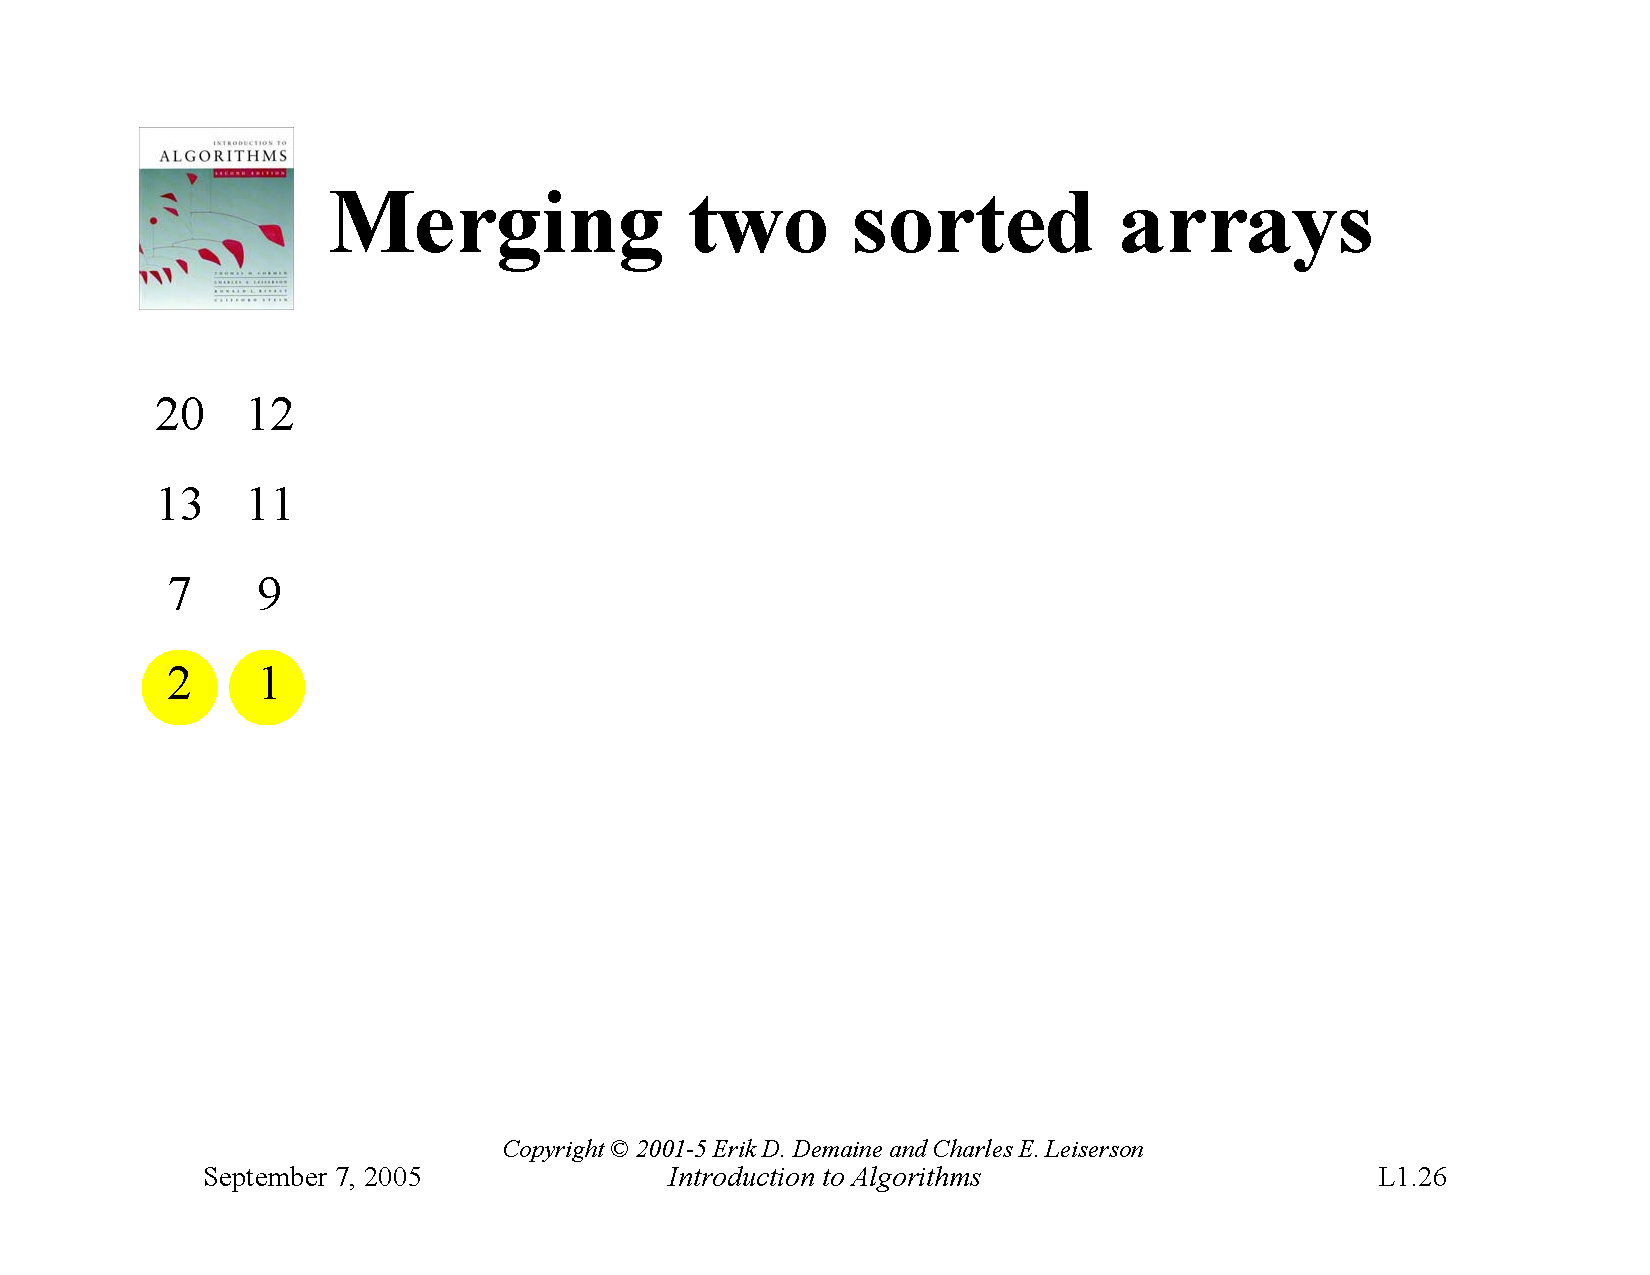
\includegraphics[width=\textwidth, trim={1.1cm 6cm 1.1cm 4.95cm}, clip]{pages/lec1_26}
\end{frame}
\begin{frame}{Merging two sorted arrays}
    \centering
    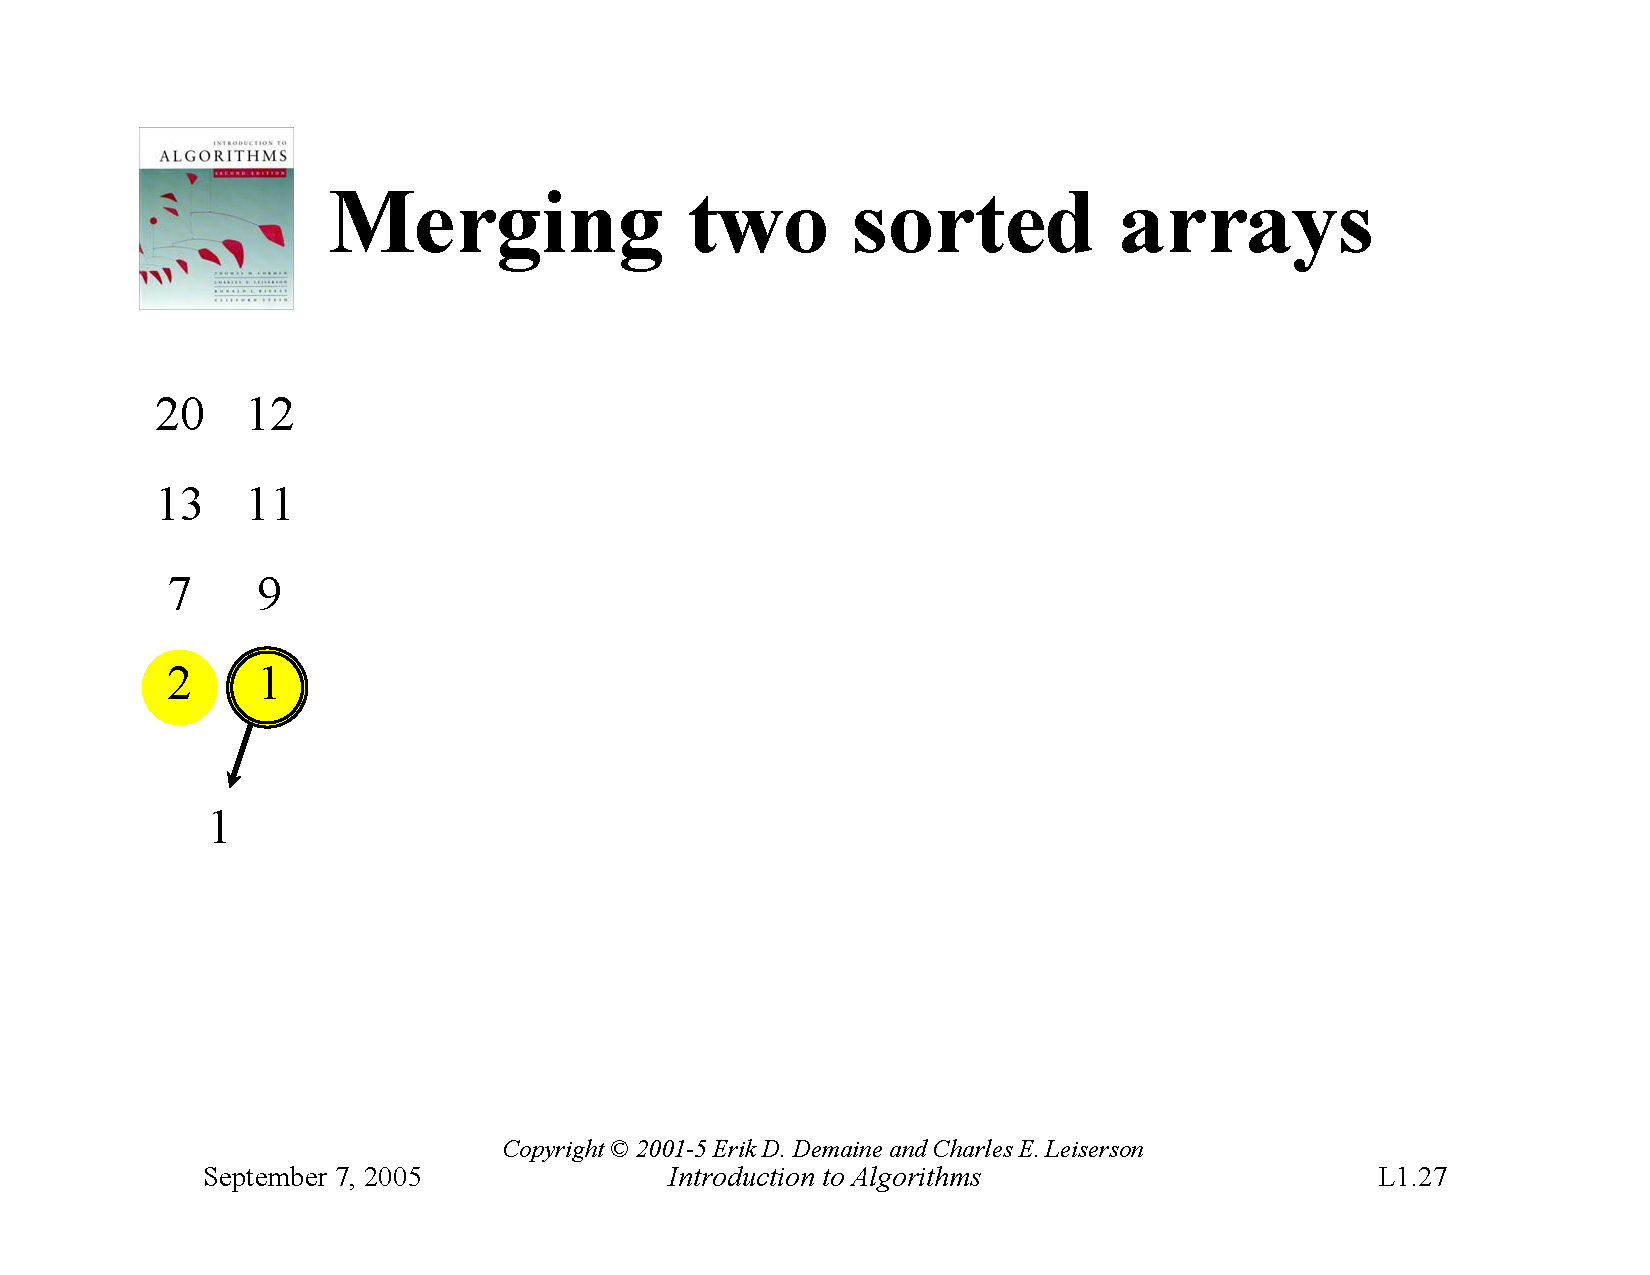
\includegraphics[width=\textwidth, trim={1.1cm 6cm 1.1cm 4.95cm}, clip]{pages/lec1_27}
\end{frame}
\begin{frame}{Merging two sorted arrays}
    \centering
    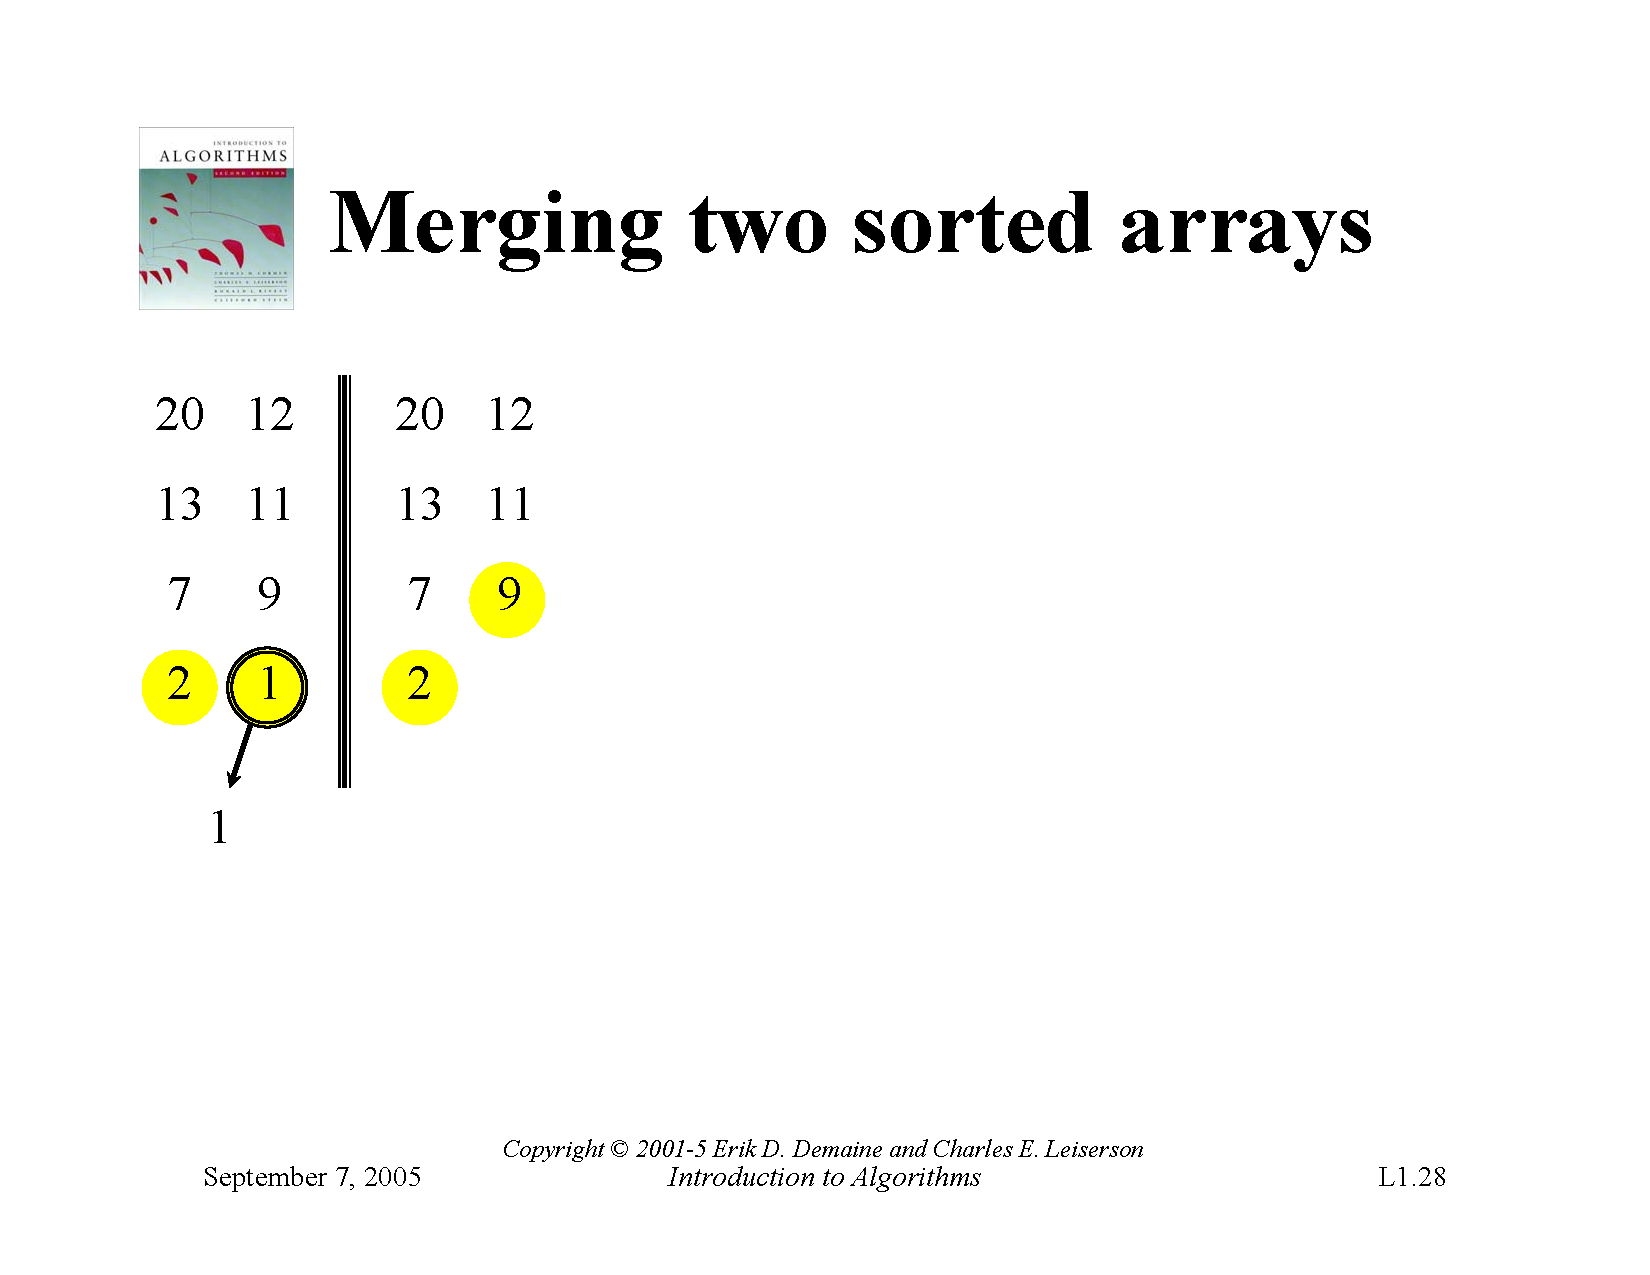
\includegraphics[width=\textwidth, trim={1.1cm 6cm 1.1cm 4.95cm}, clip]{pages/lec1_28}
\end{frame}
\begin{frame}{Merging two sorted arrays}
    \centering
    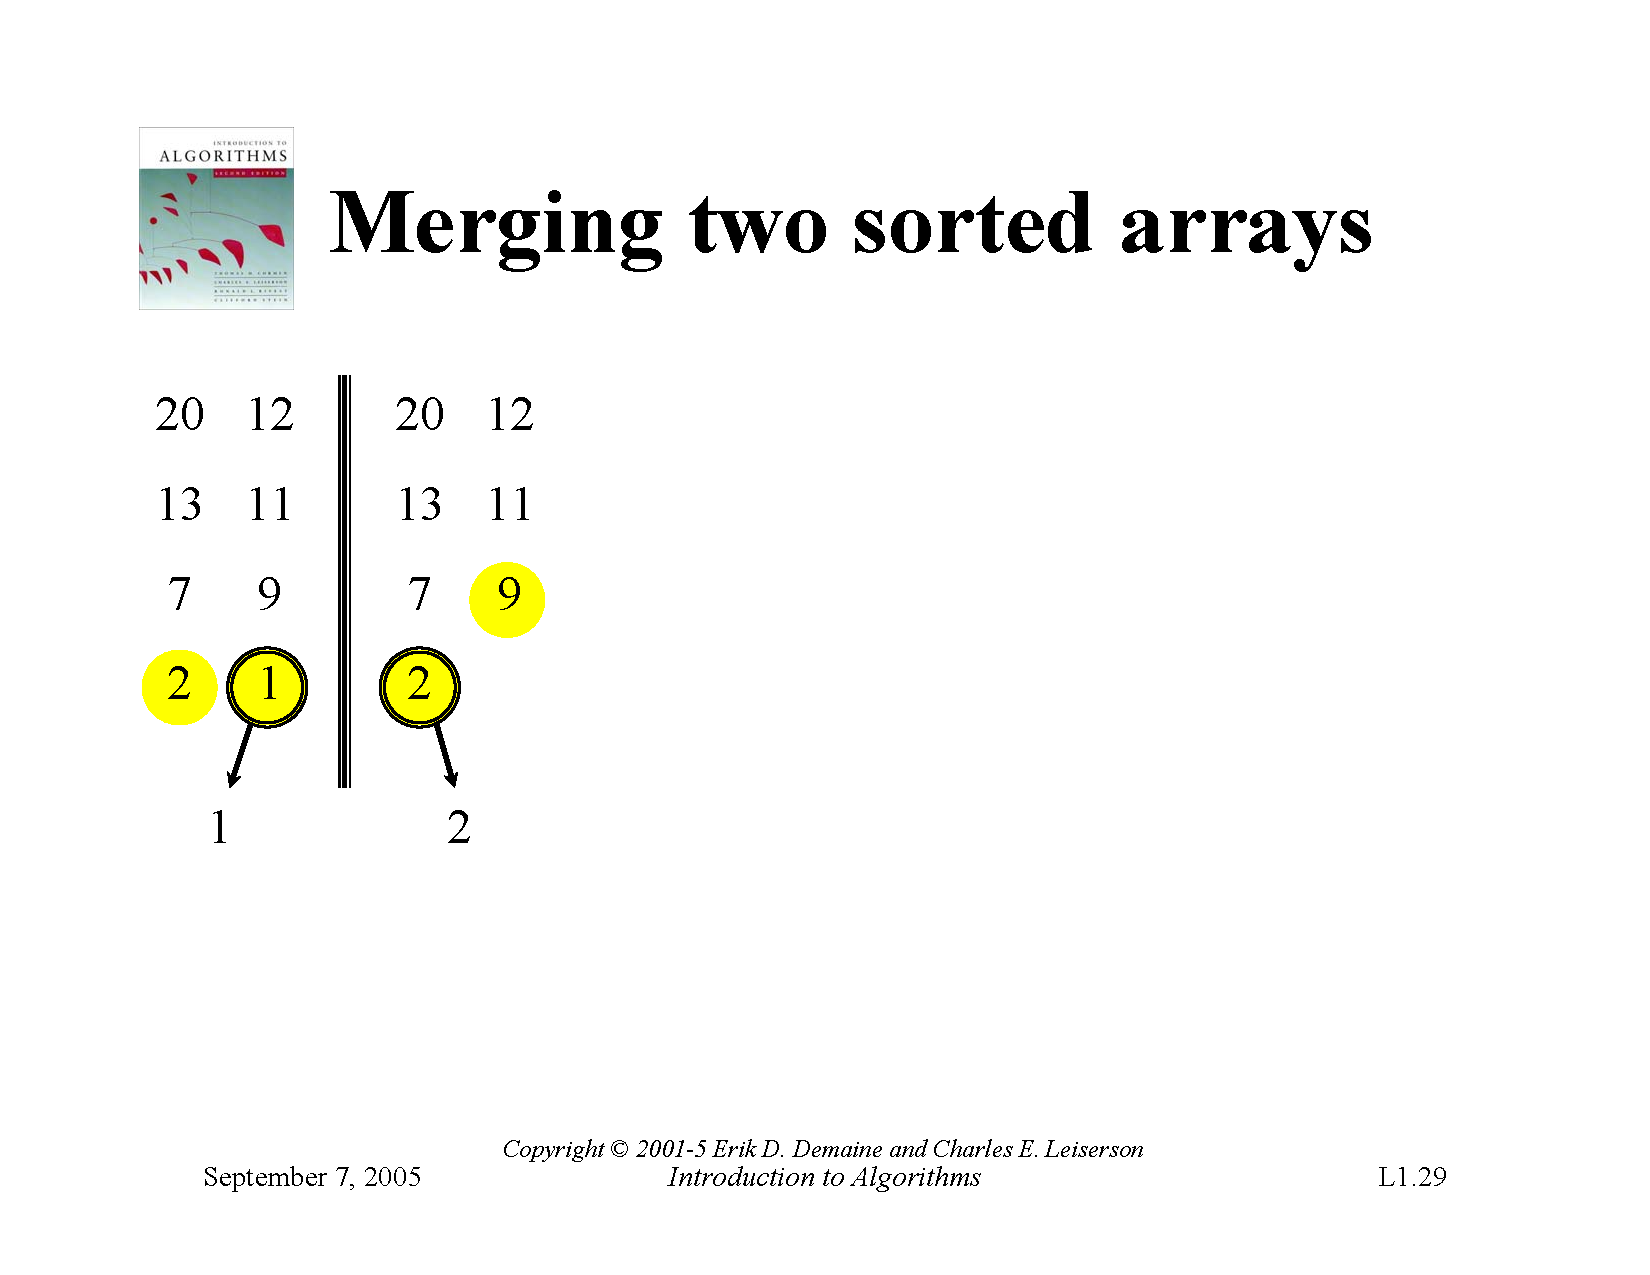
\includegraphics[width=\textwidth, trim={1.1cm 6cm 1.1cm 4.95cm}, clip]{pages/lec1_29}
\end{frame}
\begin{frame}{Merging two sorted arrays}
    \centering
    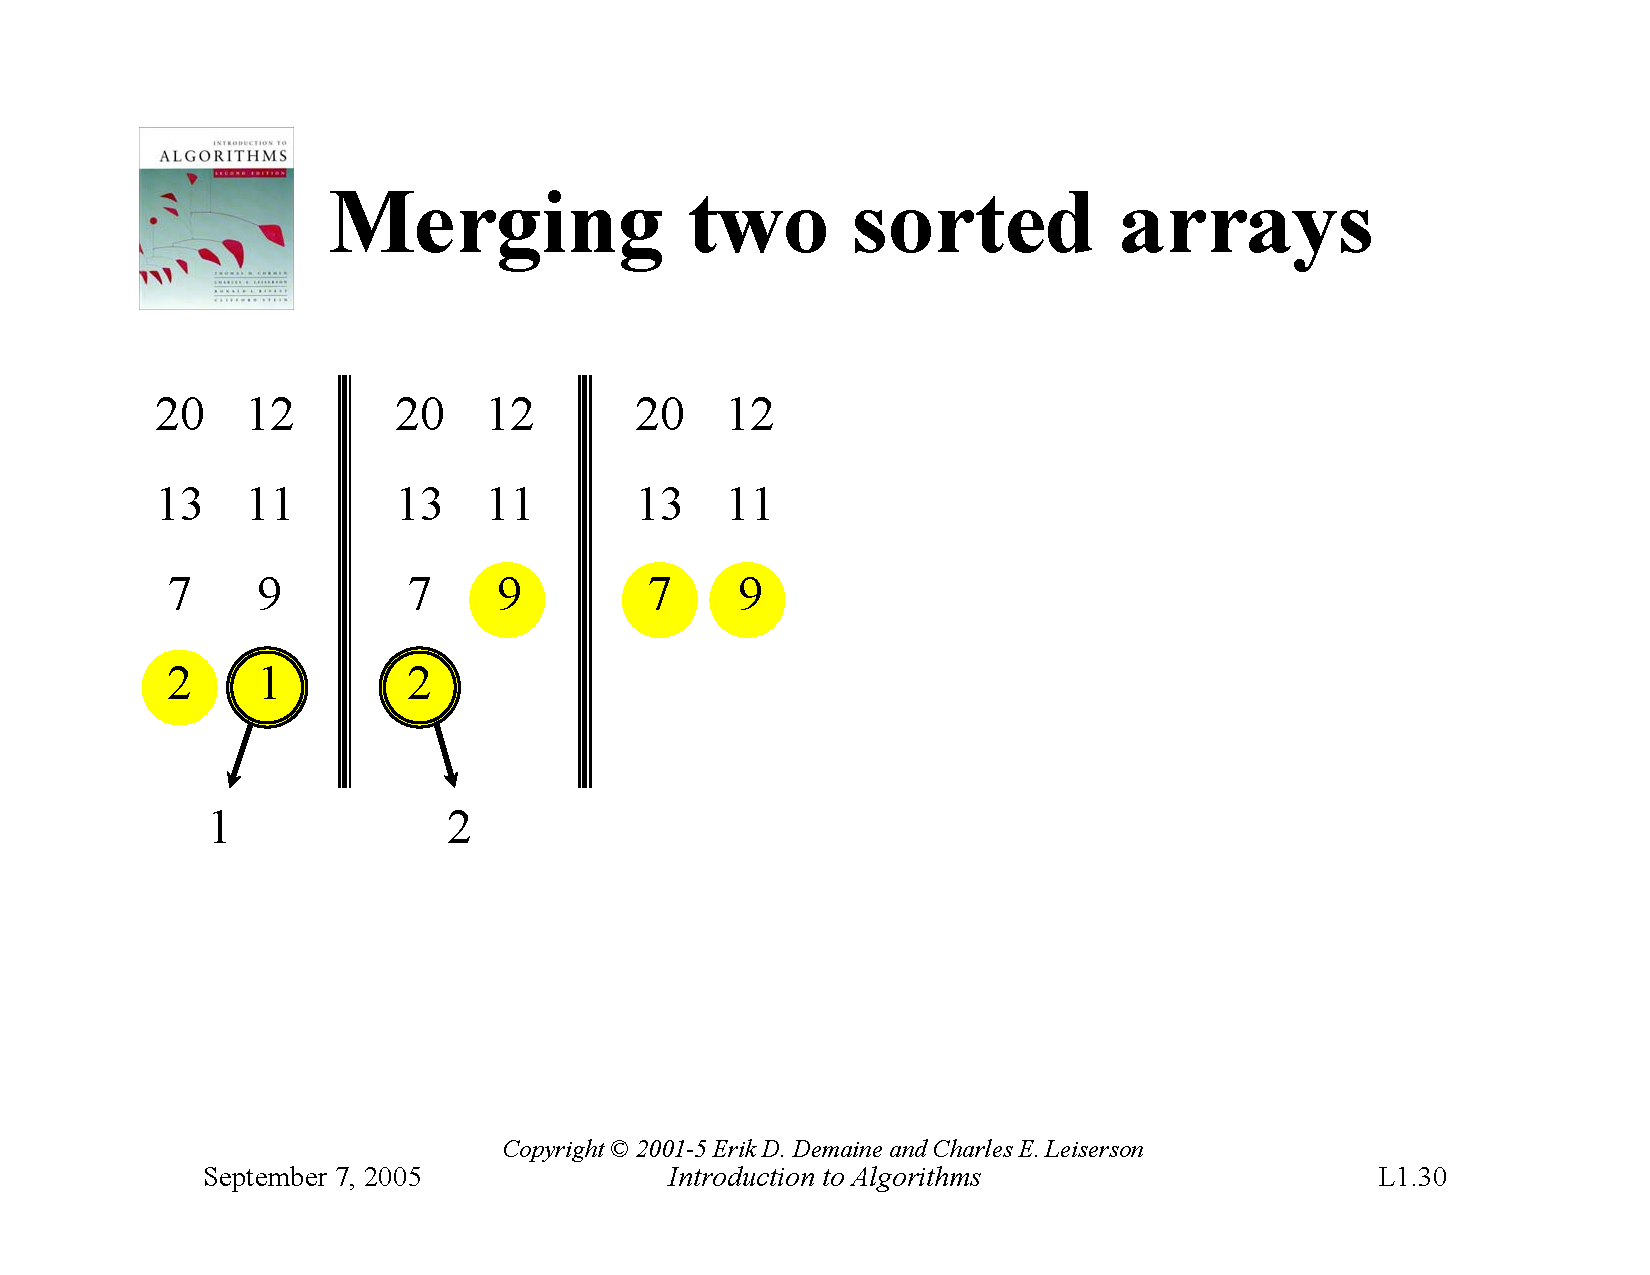
\includegraphics[width=\textwidth, trim={1.1cm 6cm 1.1cm 4.95cm}, clip]{pages/lec1_30}
\end{frame}
\begin{frame}{Merging two sorted arrays}
    \centering
    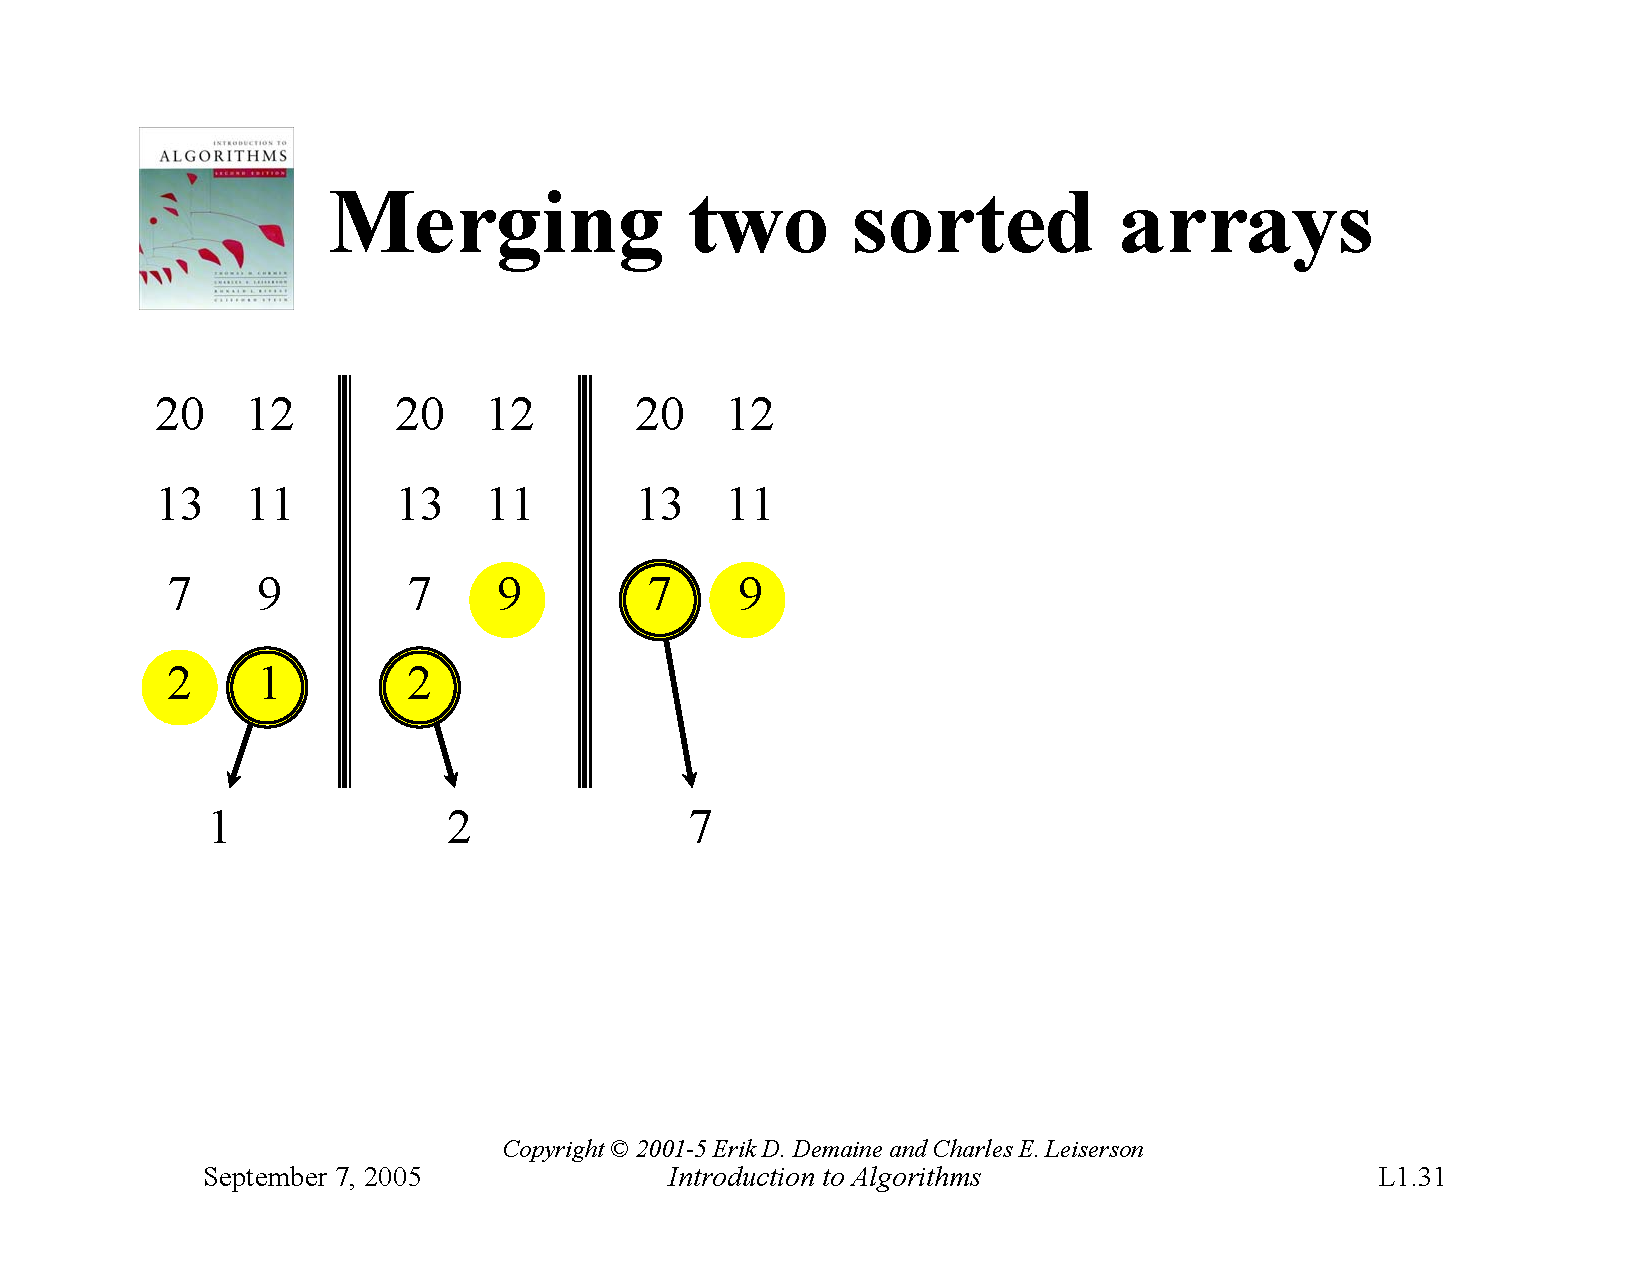
\includegraphics[width=\textwidth, trim={1.1cm 6cm 1.1cm 4.95cm}, clip]{pages/lec1_31}
\end{frame}
\begin{frame}{Merging two sorted arrays}
    \centering
    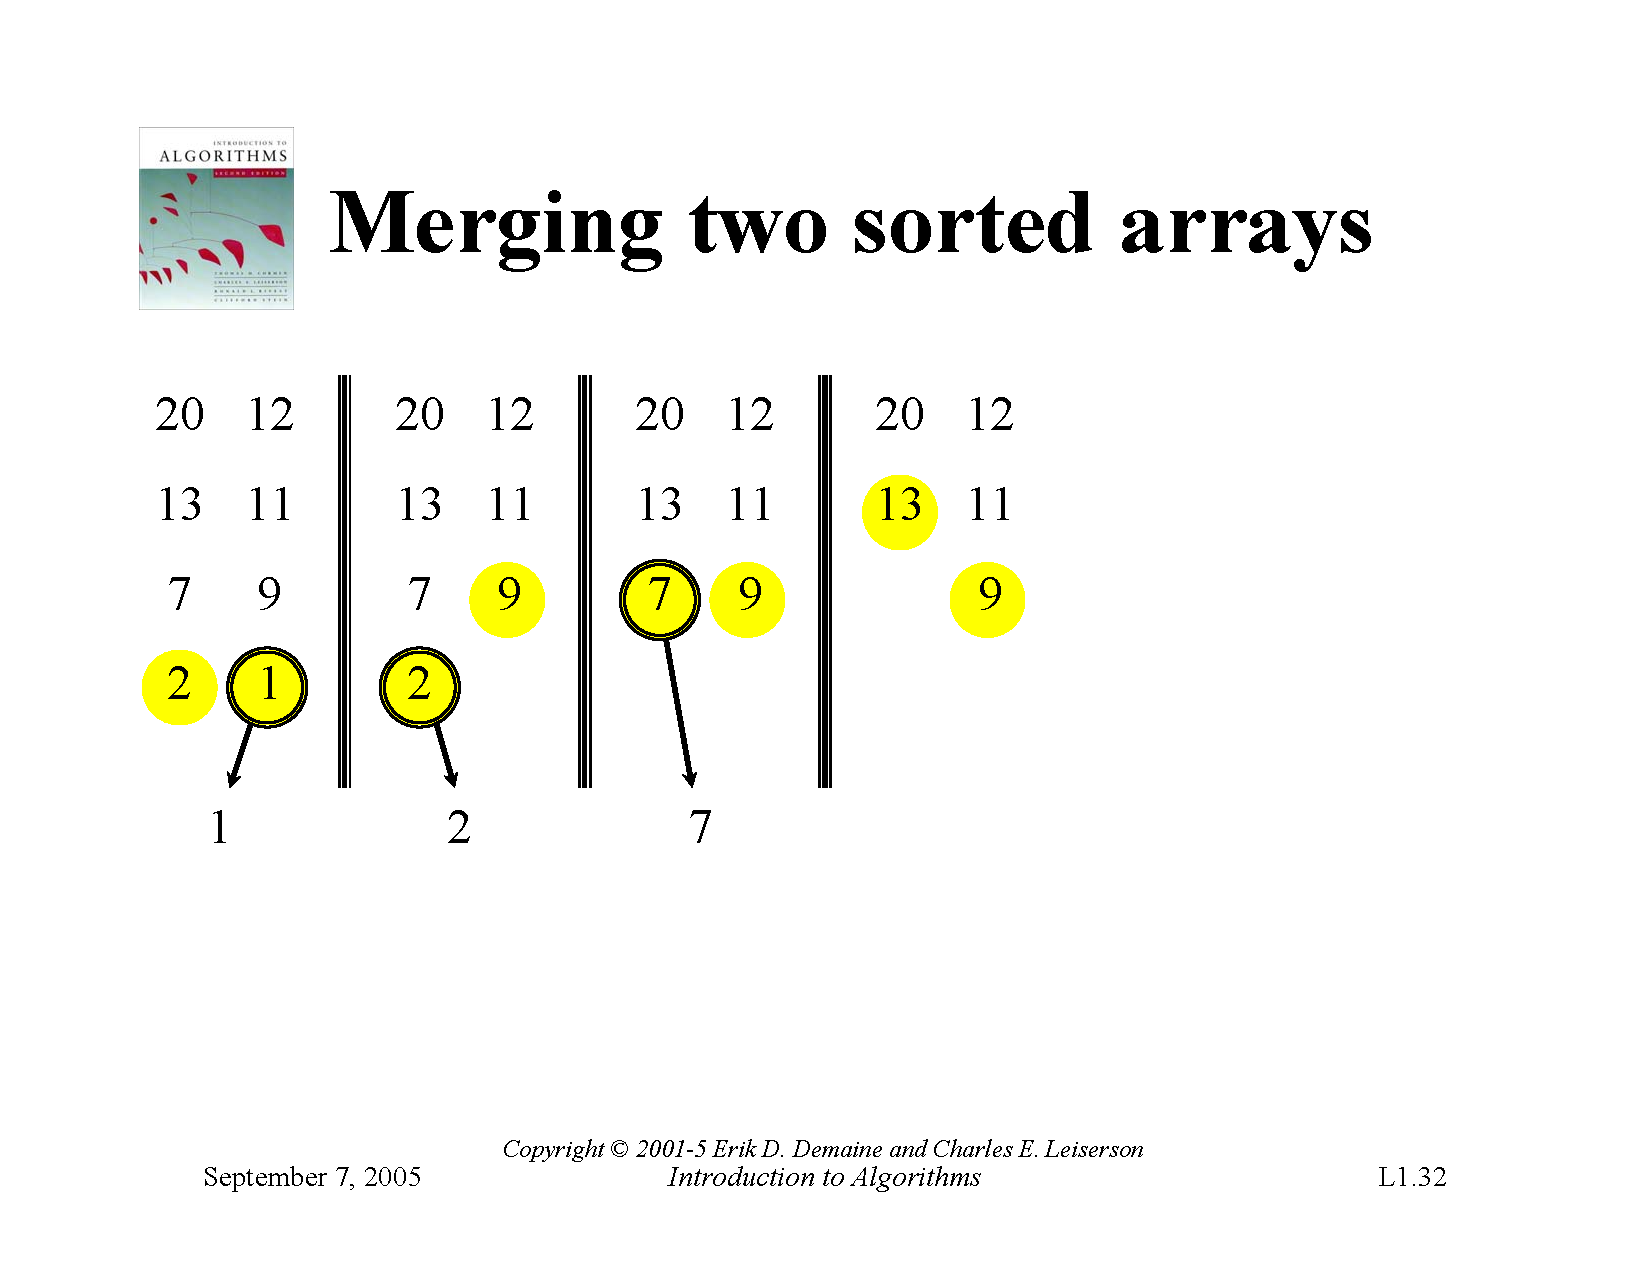
\includegraphics[width=\textwidth, trim={1.1cm 6cm 1.1cm 4.95cm}, clip]{pages/lec1_32}
\end{frame}
\begin{frame}{Merging two sorted arrays}
    \centering
    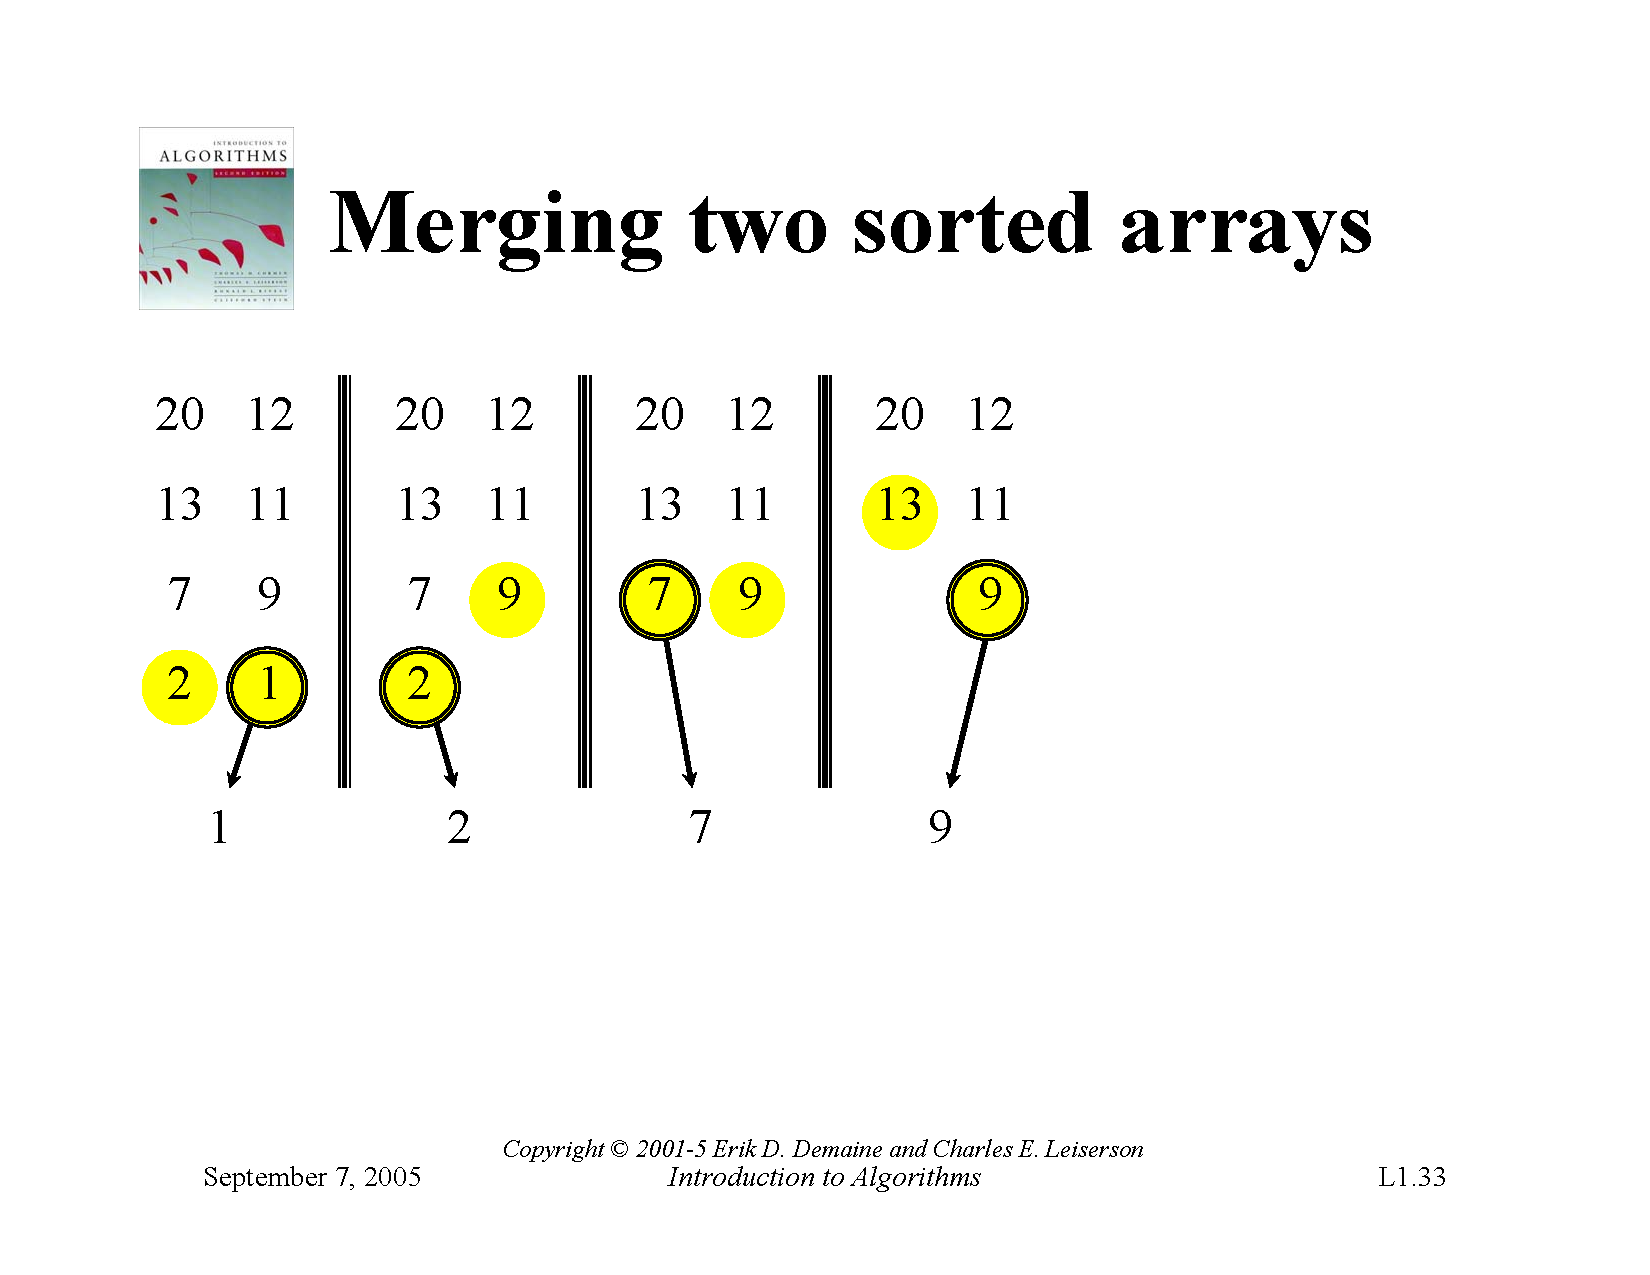
\includegraphics[width=\textwidth, trim={1.1cm 6cm 1.1cm 4.95cm}, clip]{pages/lec1_33}
\end{frame}
\begin{frame}{Merging two sorted arrays}
    \centering
    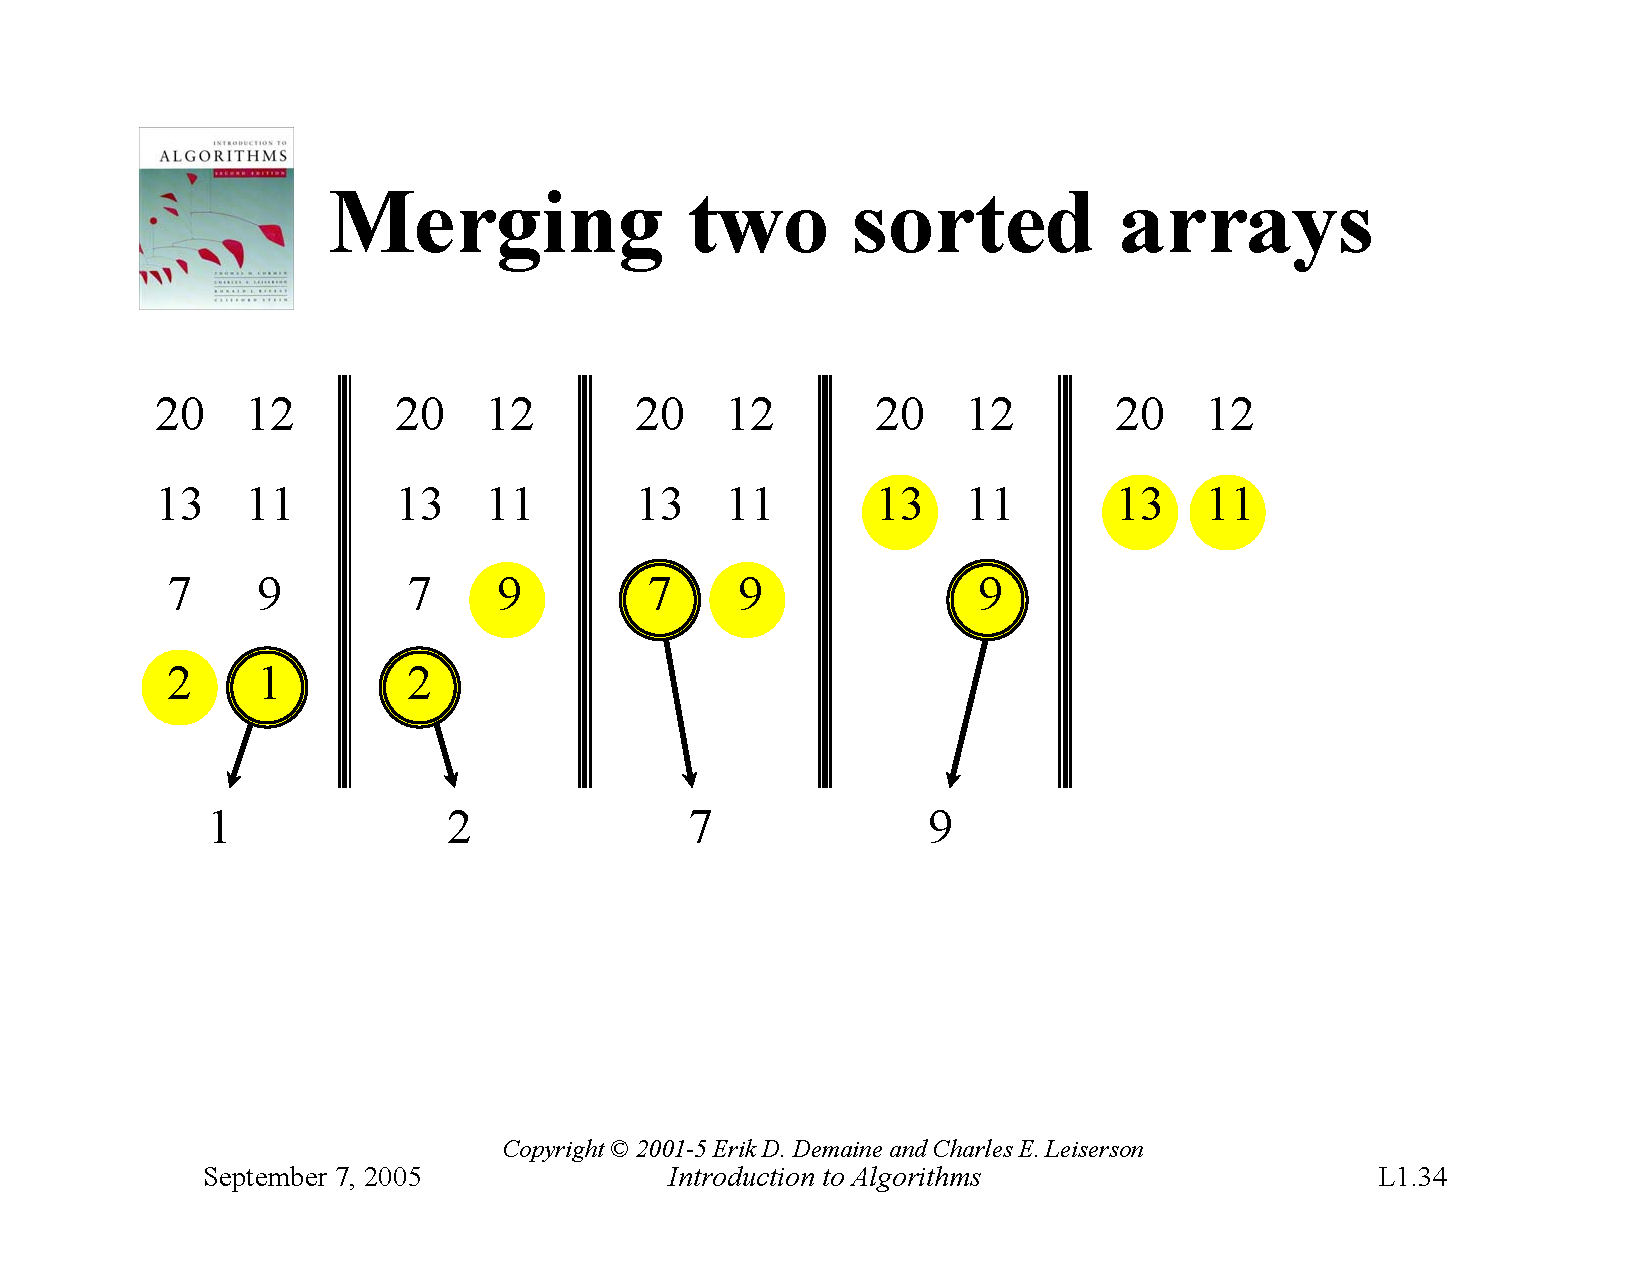
\includegraphics[width=\textwidth, trim={1.1cm 6cm 1.1cm 4.95cm}, clip]{pages/lec1_34}
\end{frame}
\begin{frame}{Merging two sorted arrays}
    \centering
    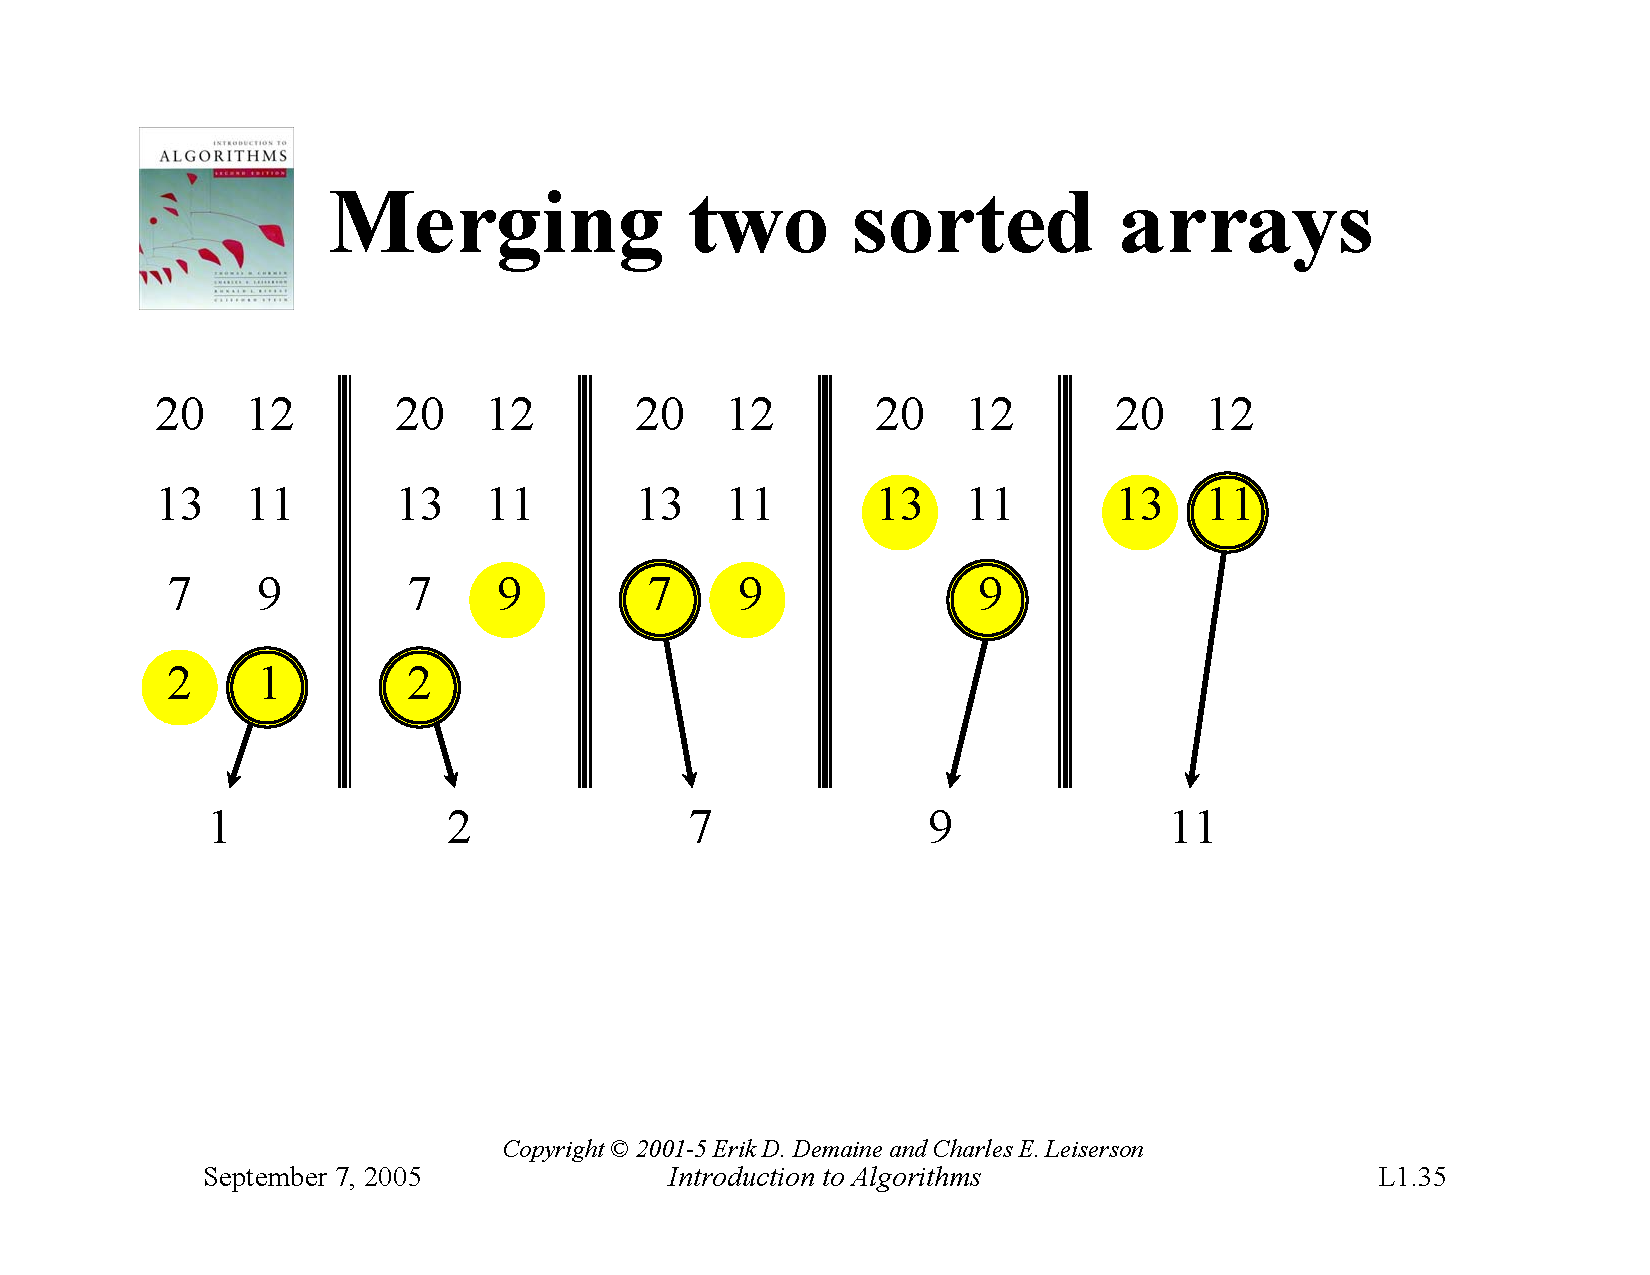
\includegraphics[width=\textwidth, trim={1.1cm 6cm 1.1cm 4.95cm}, clip]{pages/lec1_35}
\end{frame}
\begin{frame}{Merging two sorted arrays}
    \centering
    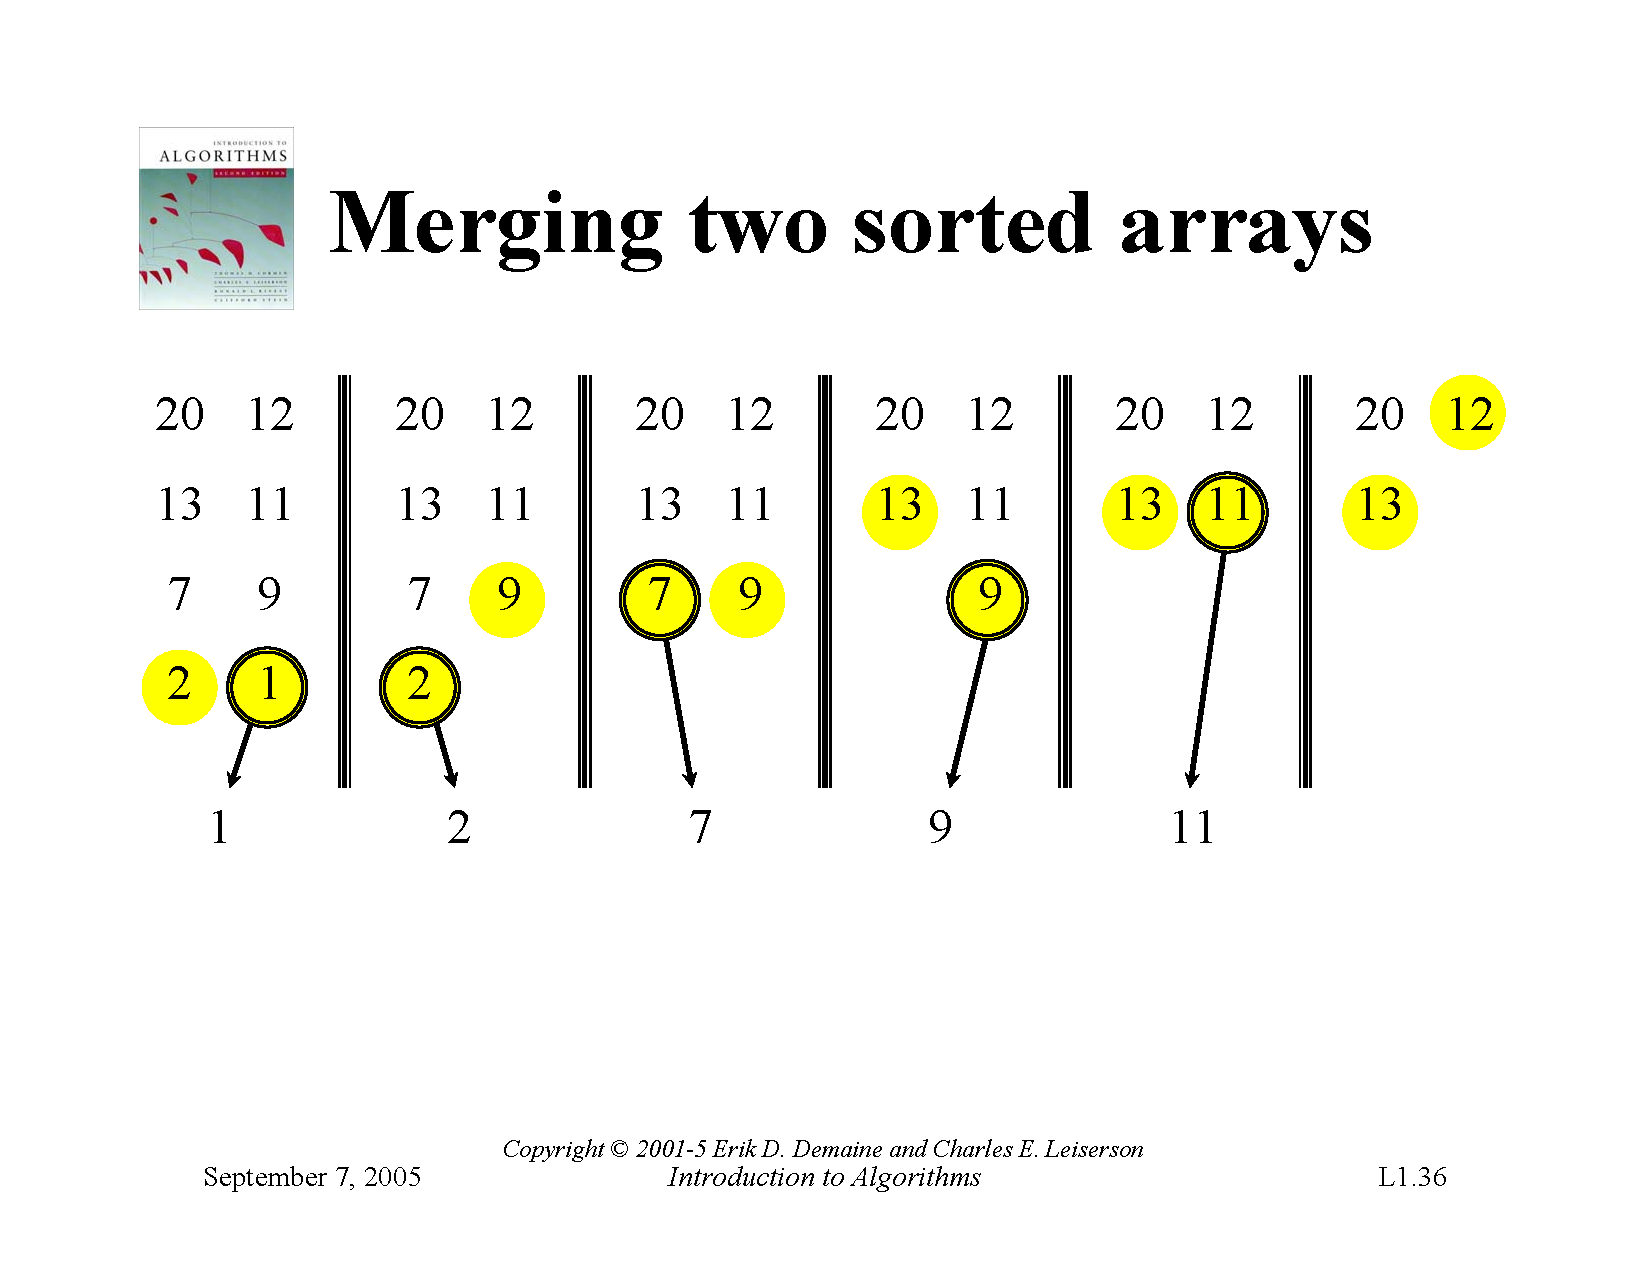
\includegraphics[width=\textwidth, trim={1.1cm 6cm 1.1cm 4.95cm}, clip]{pages/lec1_36}
\end{frame}
\begin{frame}{Merging two sorted arrays}
    \centering
    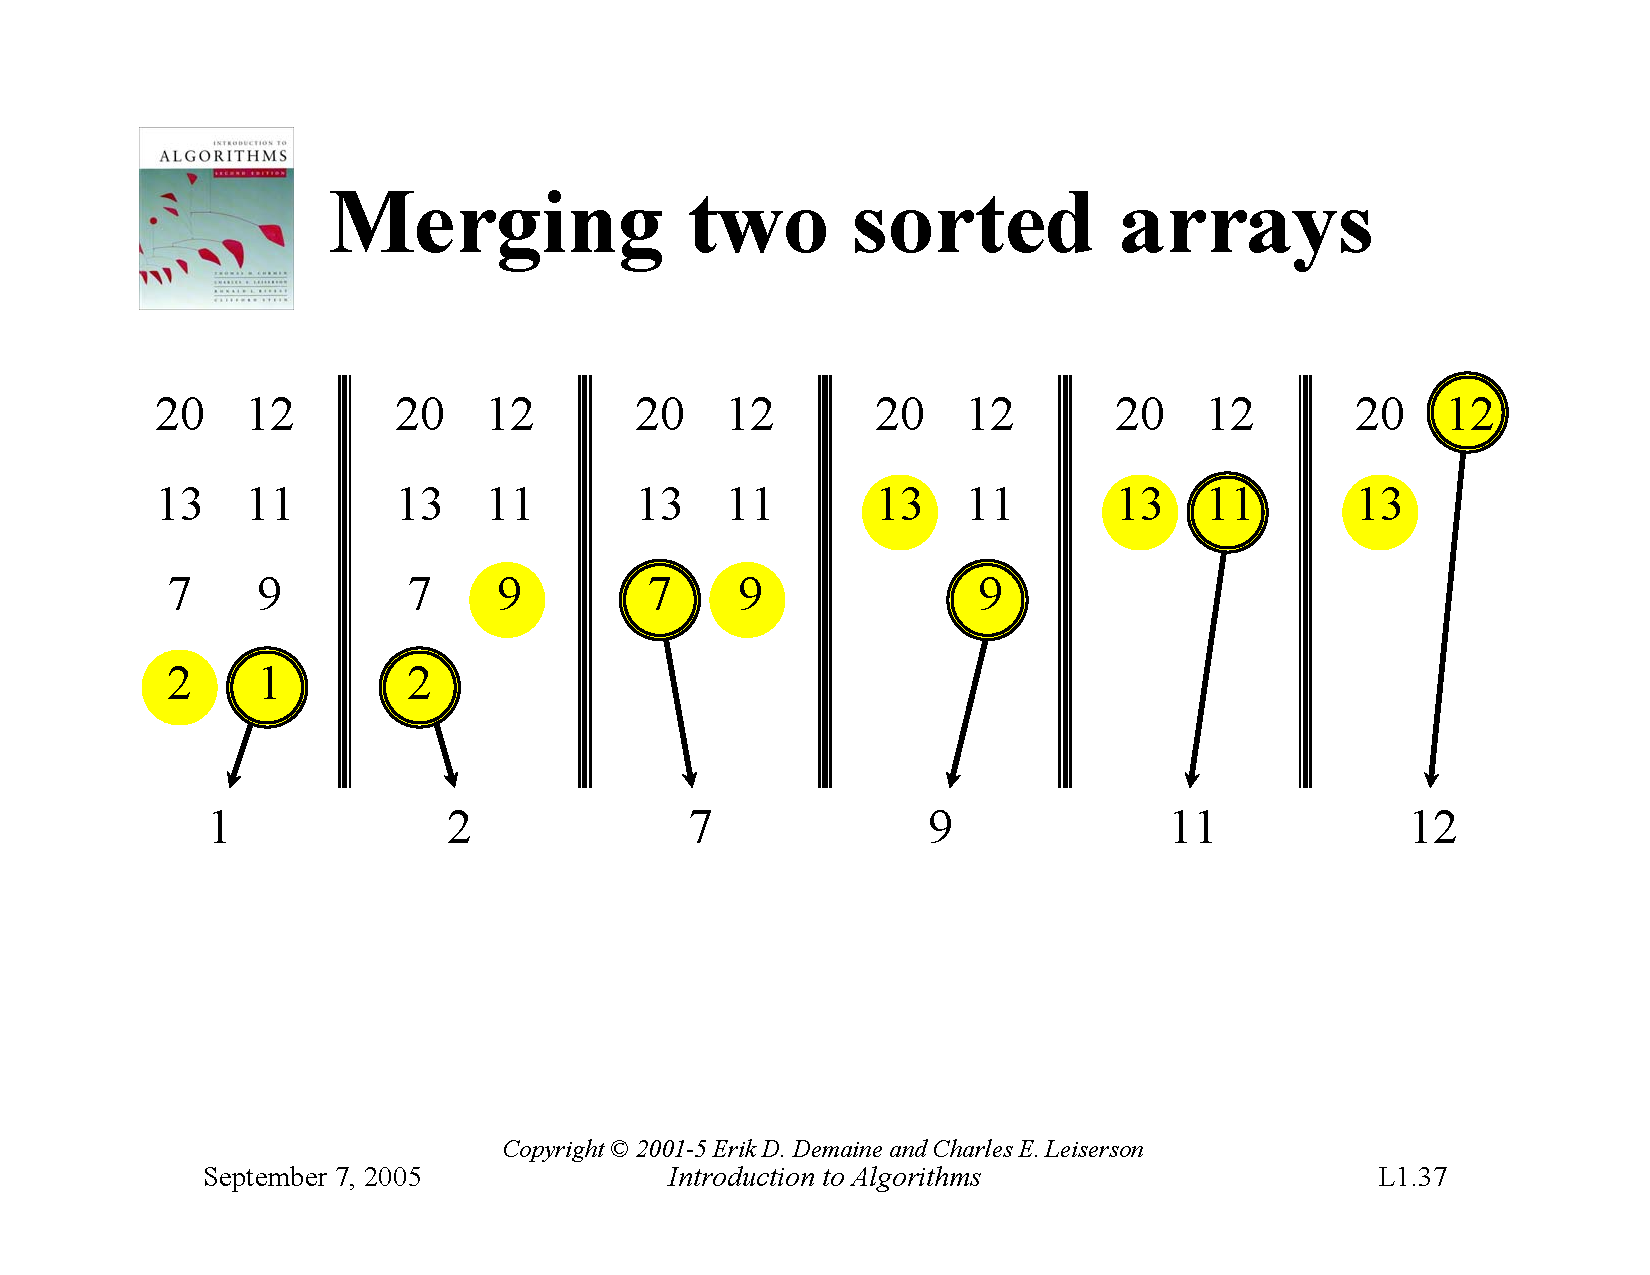
\includegraphics[width=\textwidth, trim={1.1cm 6cm 1.1cm 4.95cm}, clip]{pages/lec1_37}
\end{frame}
\begin{frame}{Merging two sorted arrays}
    \centering
    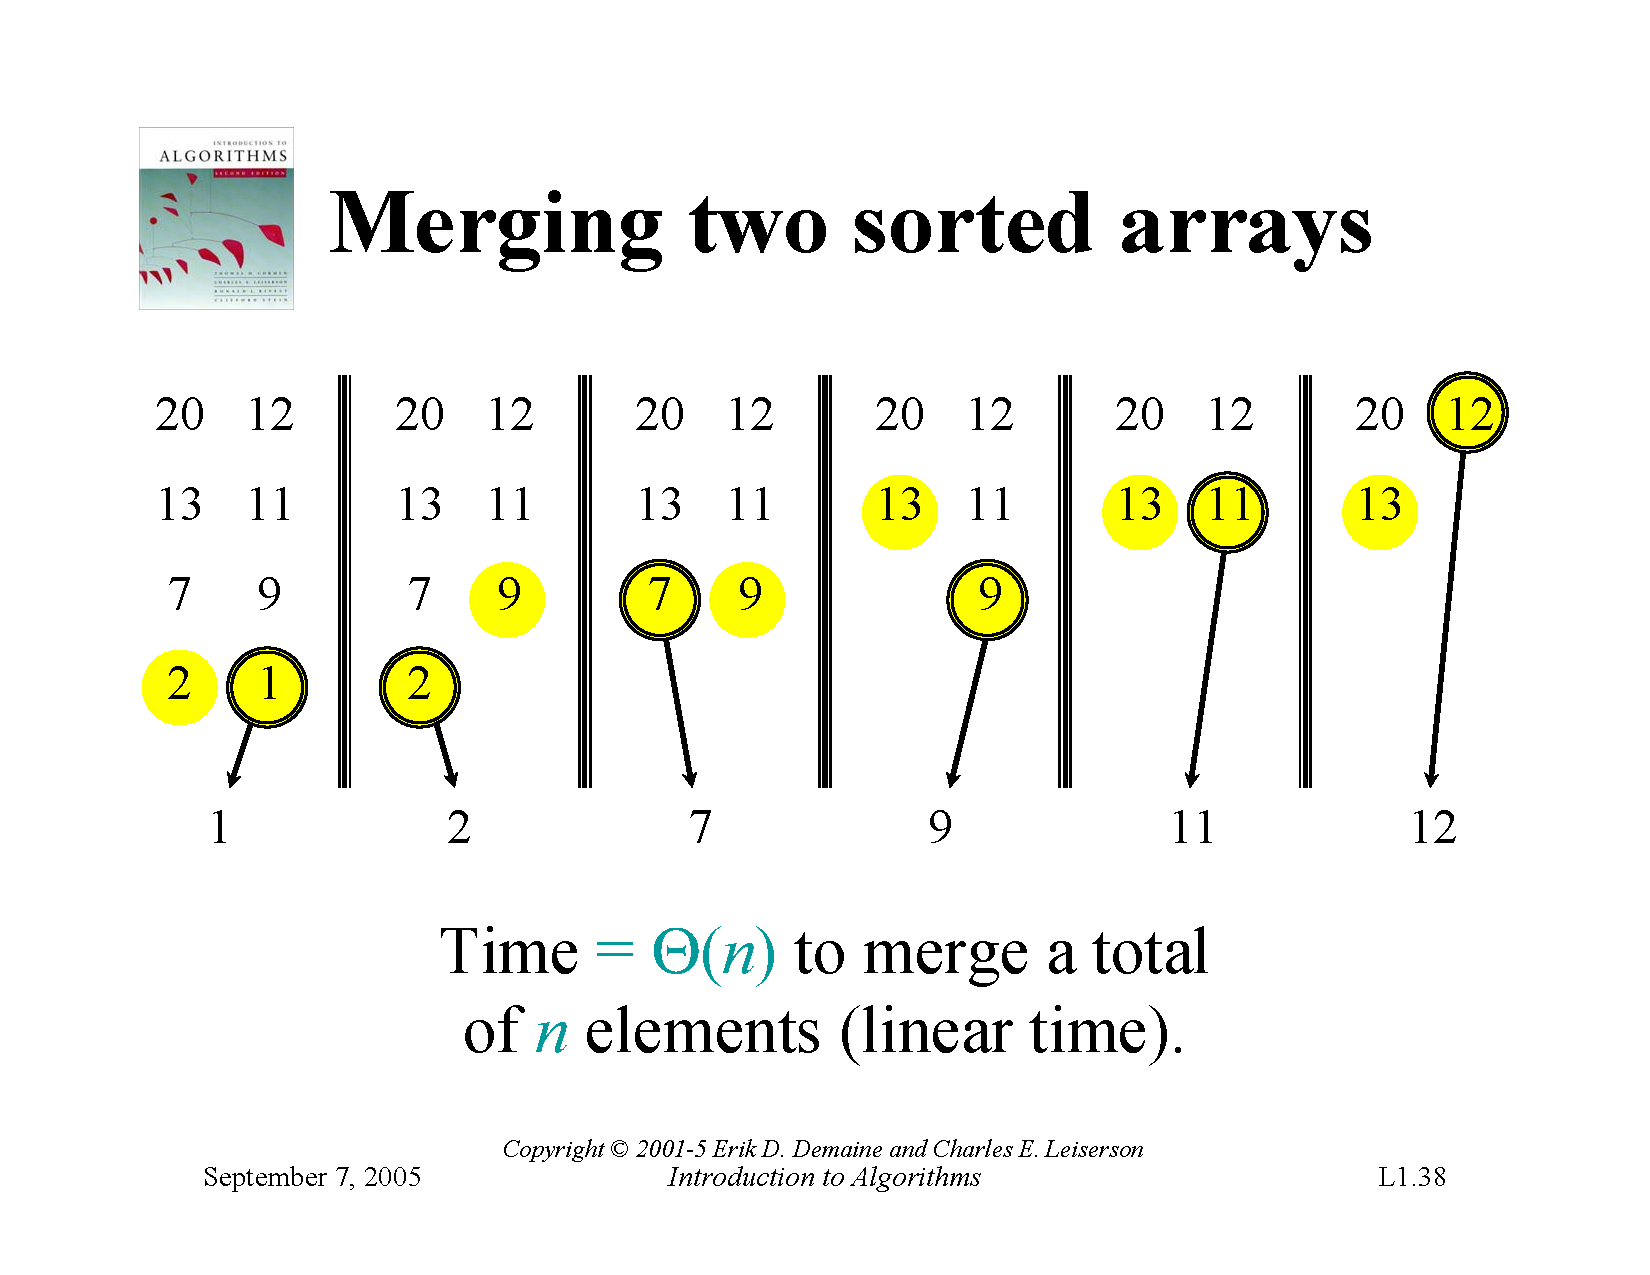
\includegraphics[width=\textwidth, trim={1.1cm 6cm 1.1cm 4.95cm}, clip]{pages/lec1_38}\\
    \vspace{2mm}
    Time$= \Theta(n)$ to merge a total of $n$ elements (linear time).
\end{frame}

\begin{frame}{Analyzing merge-sort} 
    \large \textbf{Abuse!} \\
    \vspace{10mm}
    \Large
    \begin{tabular}{r | l}
        $T(n)$                         & \textsc{Merge-sort} $A[1 \ldots n]$ \\
        $\Theta(1)$                 & \hspace{1em} 1. \textbf{if} $n = 1$, done! \\
        $2T(\frac{n}{2})$       & \hspace{1em} 2. Recursively sort $A[ 1 \ldots \lceil \frac{n}{2} \rceil ]$ \\
                                         & \hspace{2em}      and $A[ \lceil \frac{n}{2} \rceil + 1 \ldots n ]$. \\
        $\Theta(n)$                 & \hspace{1em} 3. \textsc{Merge} the 2 sorted lists. 
    \end{tabular} \\
    \vspace{10mm}
    {\large \textbf{Sloppiness:} Should be $T(\lceil \frac{n}{2} \rceil) + T(\lfloor \frac{n}{2} \rfloor)$, but it turns out not matter asymptotically.}
    \begin{tikzpicture}[remember picture,overlay]   %% use here too
        \draw[red,thick,->] (-5, 6.3) to [out=180,in=180] (-4.6, 4.25);
        \draw[blue,thick,->] (-5.1, 0.76) to [out=150,in=180] (-4.9, 3.6);
    \end{tikzpicture}    
\end{frame}

\section{Recurrences}

\begin{frame}{Recurrence for merge-sort}
    \centering
    $$
        T(n) =
            \begin{cases}
                \Theta(1) \text{ \textbf{if} } n = 1 \\
                2T(\frac{n}{2}) + \Theta(n)  \text{ \textbf{if} }  n > 1. \\
            \end{cases}       
    $$
    \begin{itemize}
        \item We shall usually omit stating the base case when $T(n) = \Theta(1)$ for sufficiently small $n$, but only when it has no effect on the asymptotic solution to the recurrence.
        \item CLRS\footnote{The book} and Lecture 2 provide several ways to find a good upper bound on $T(n)$.
    \end{itemize}

\end{frame}

\begin{frame}{Recursion Tree}
    Solve $T(n) = 2T(\frac{n}{2}) + cn$, where $c > 0$ is constant.\\
    \vspace{5mm}
    \centering
    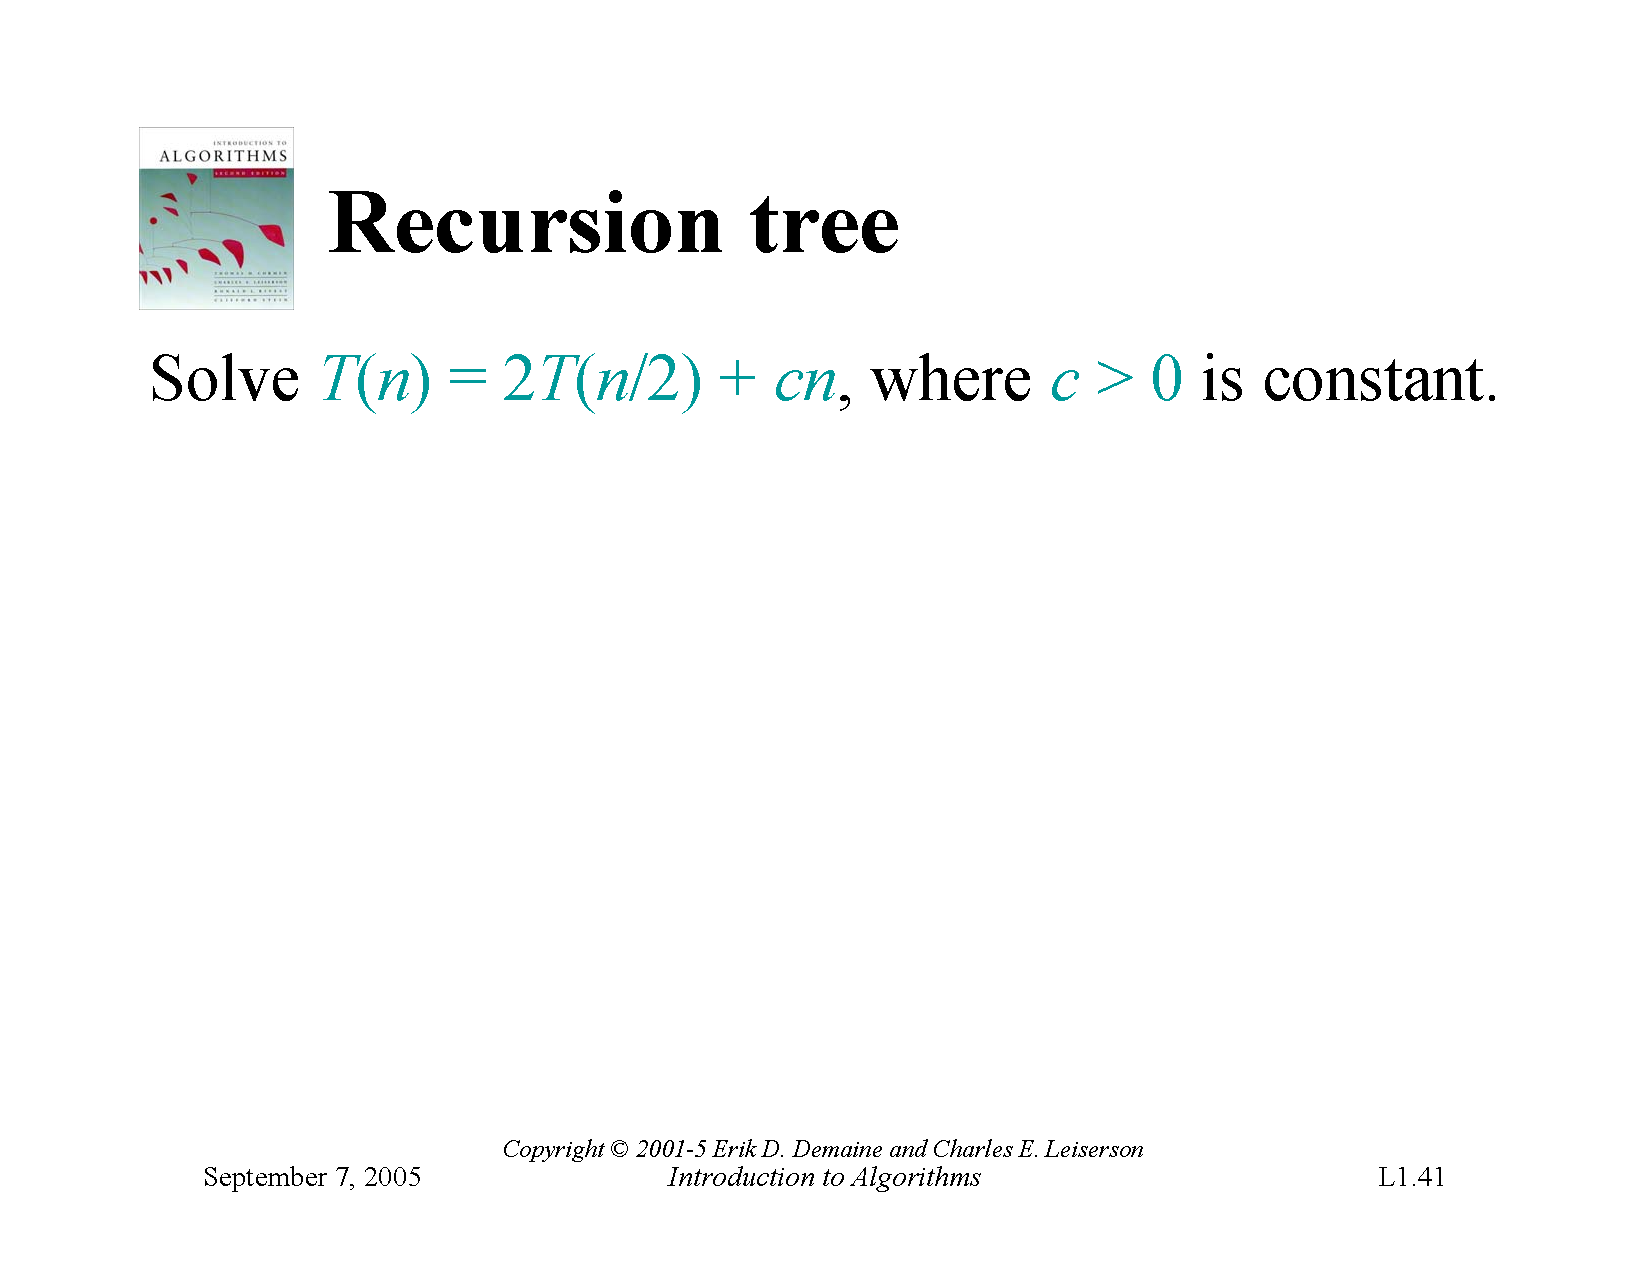
\includegraphics[width=\textwidth, trim={0.49cm 1.25cm 0.7cm 5.75cm}, clip]{pages/lec1_41}
\end{frame}
\begin{frame}{Recursion Tree}
    Solve $T(n) = 2T(\frac{n}{2}) + cn$, where $c > 0$ is constant.\\
    \vspace{5mm}
    \centering
    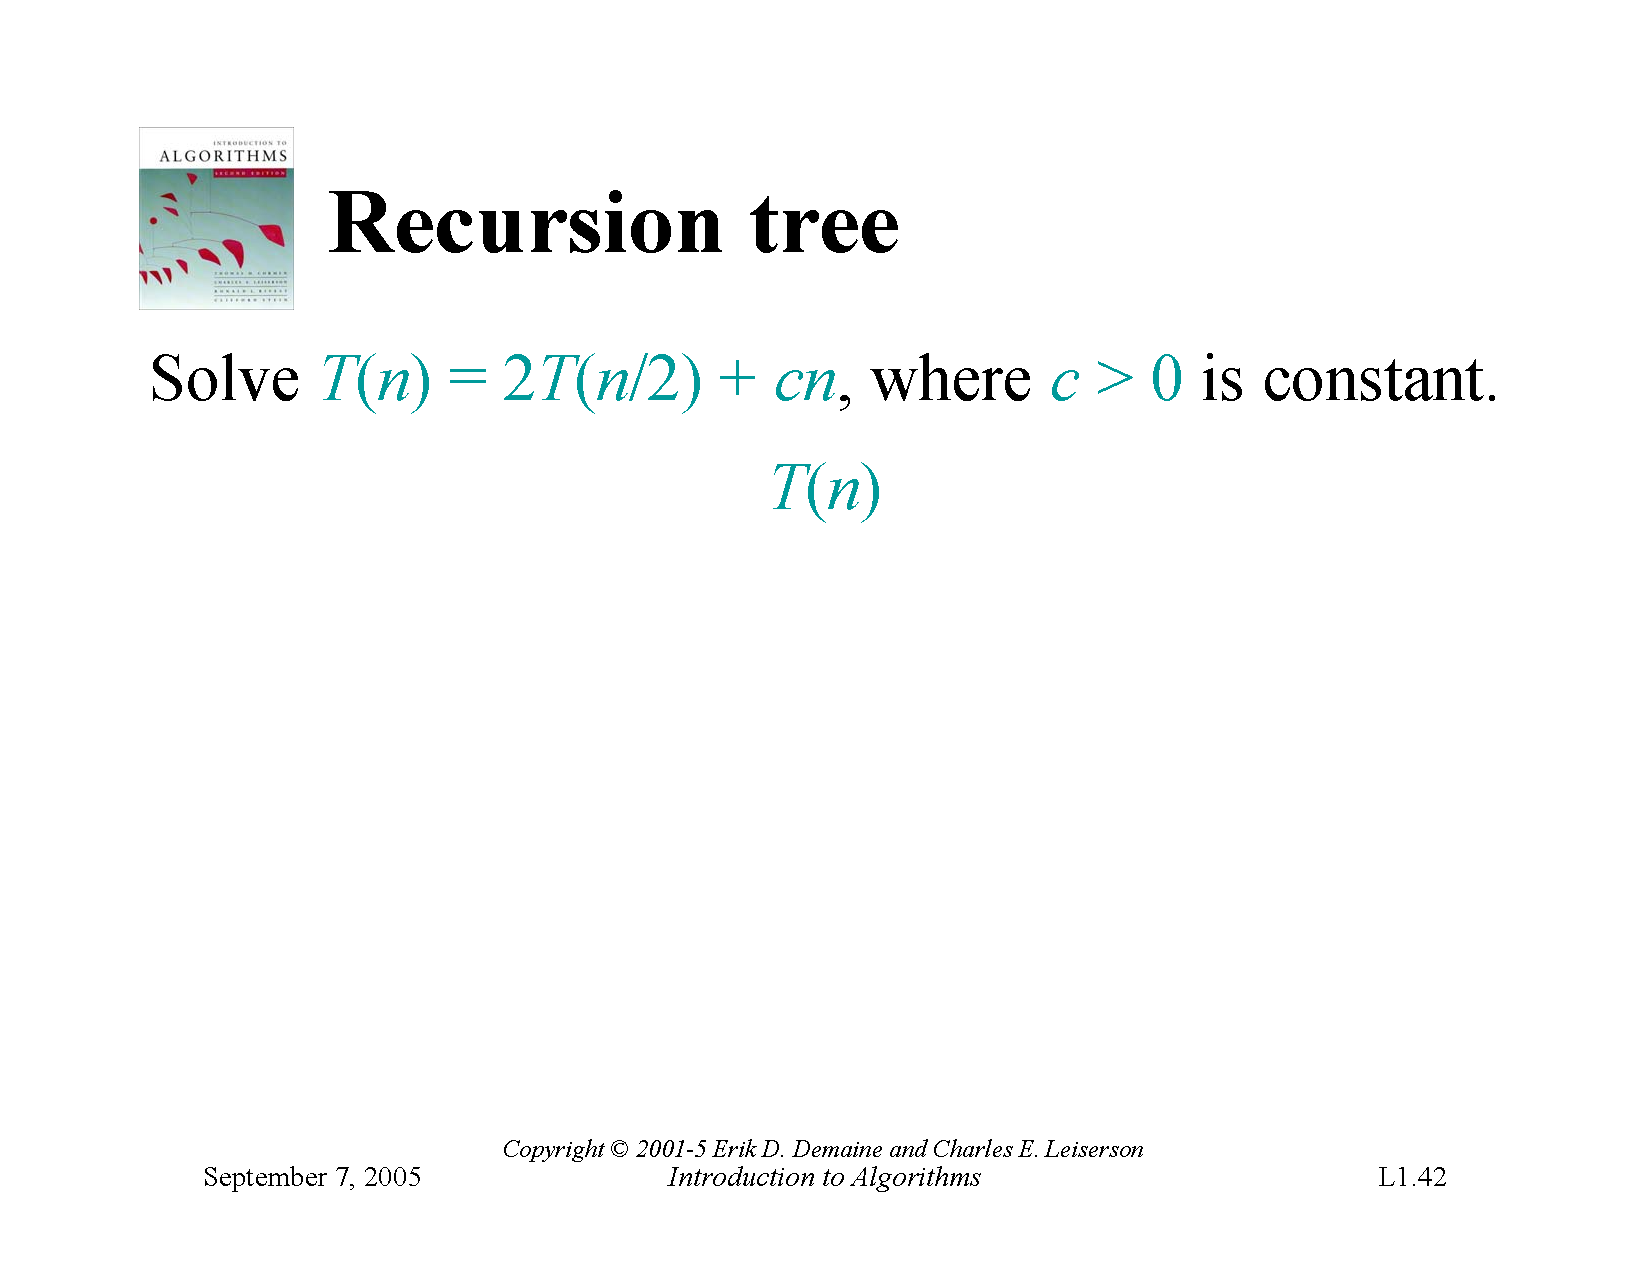
\includegraphics[width=\textwidth, trim={0.49cm 1.25cm 0.7cm 5.75cm}, clip]{pages/lec1_42}
\end{frame}
\begin{frame}{Recursion Tree}
    Solve $T(n) = 2T(\frac{n}{2}) + cn$, where $c > 0$ is constant.\\
    \vspace{5mm}
    \centering
    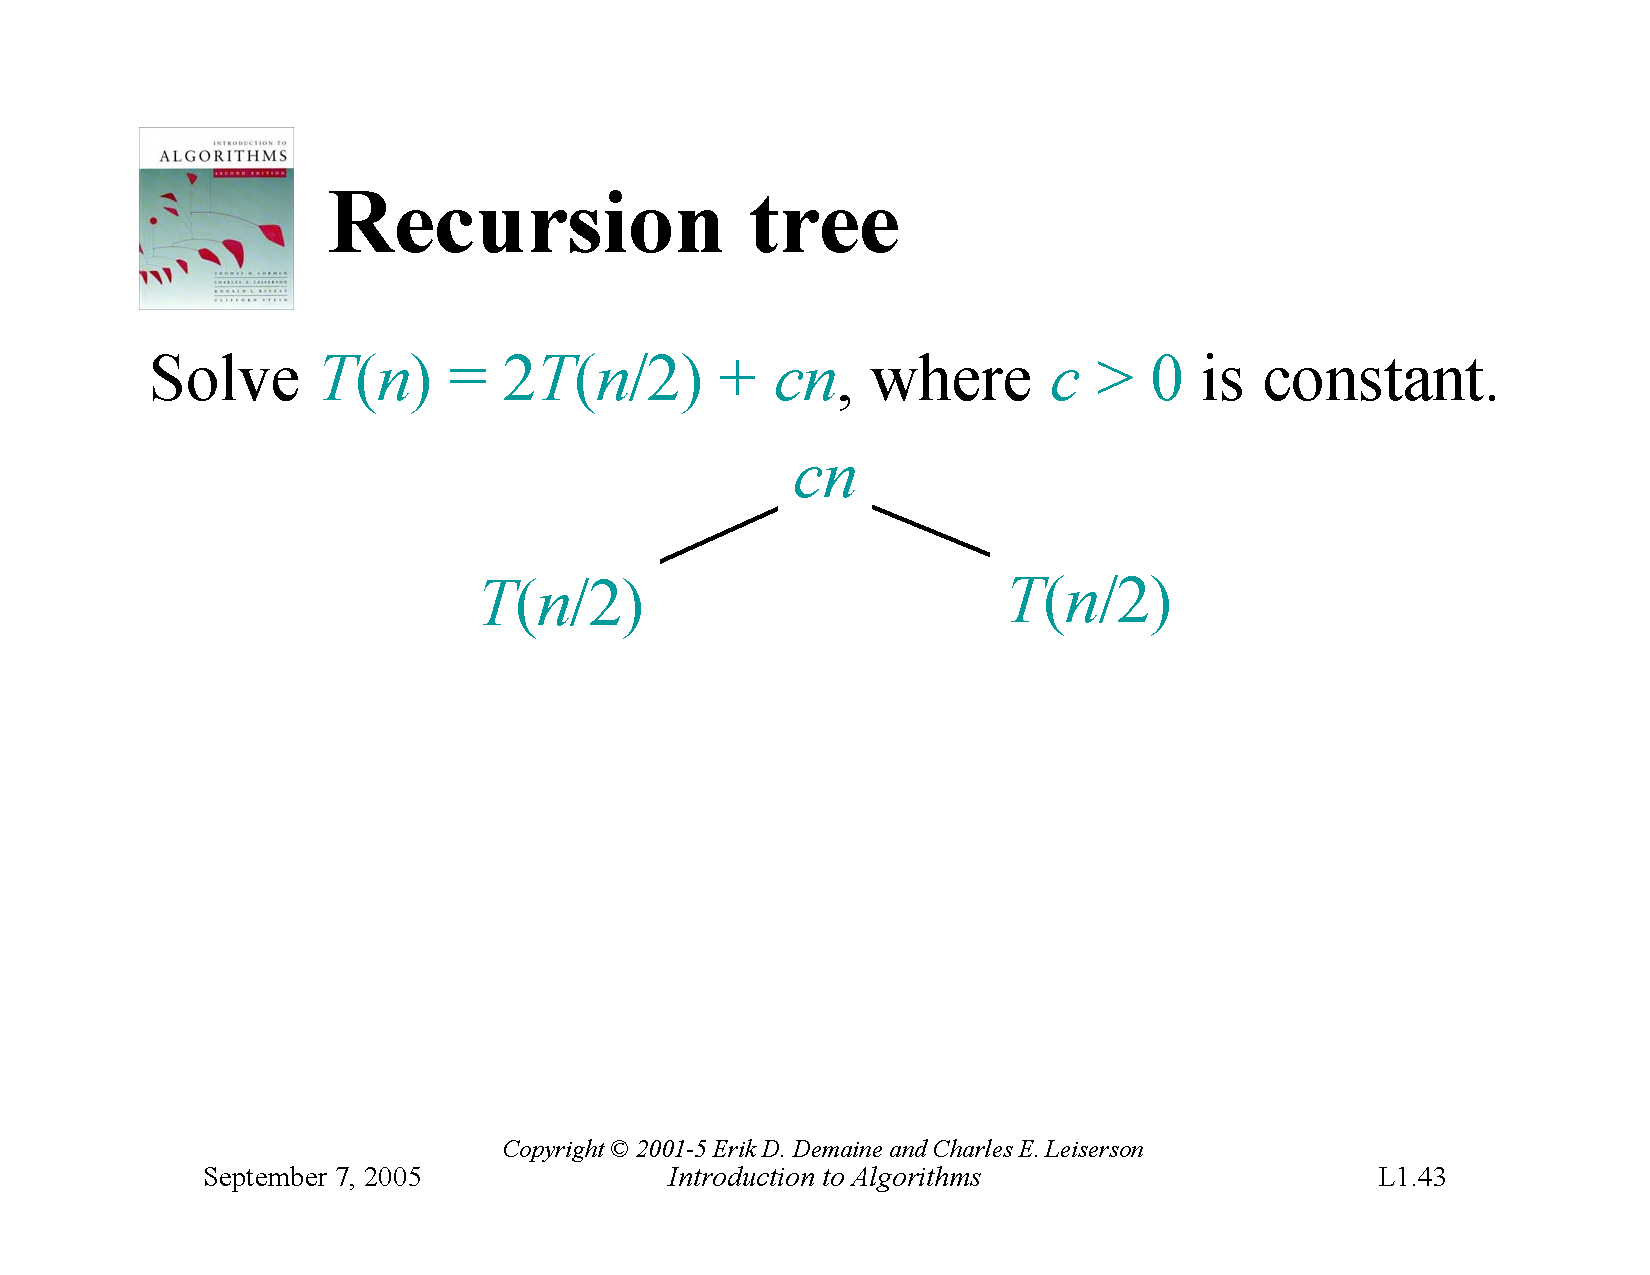
\includegraphics[width=\textwidth, trim={0.49cm 1.25cm 0.7cm 5.75cm}, clip]{pages/lec1_43}
\end{frame}
\begin{frame}{Recursion Tree}
    Solve $T(n) = 2T(\frac{n}{2}) + cn$, where $c > 0$ is constant.\\
    \vspace{5mm}
    \centering
    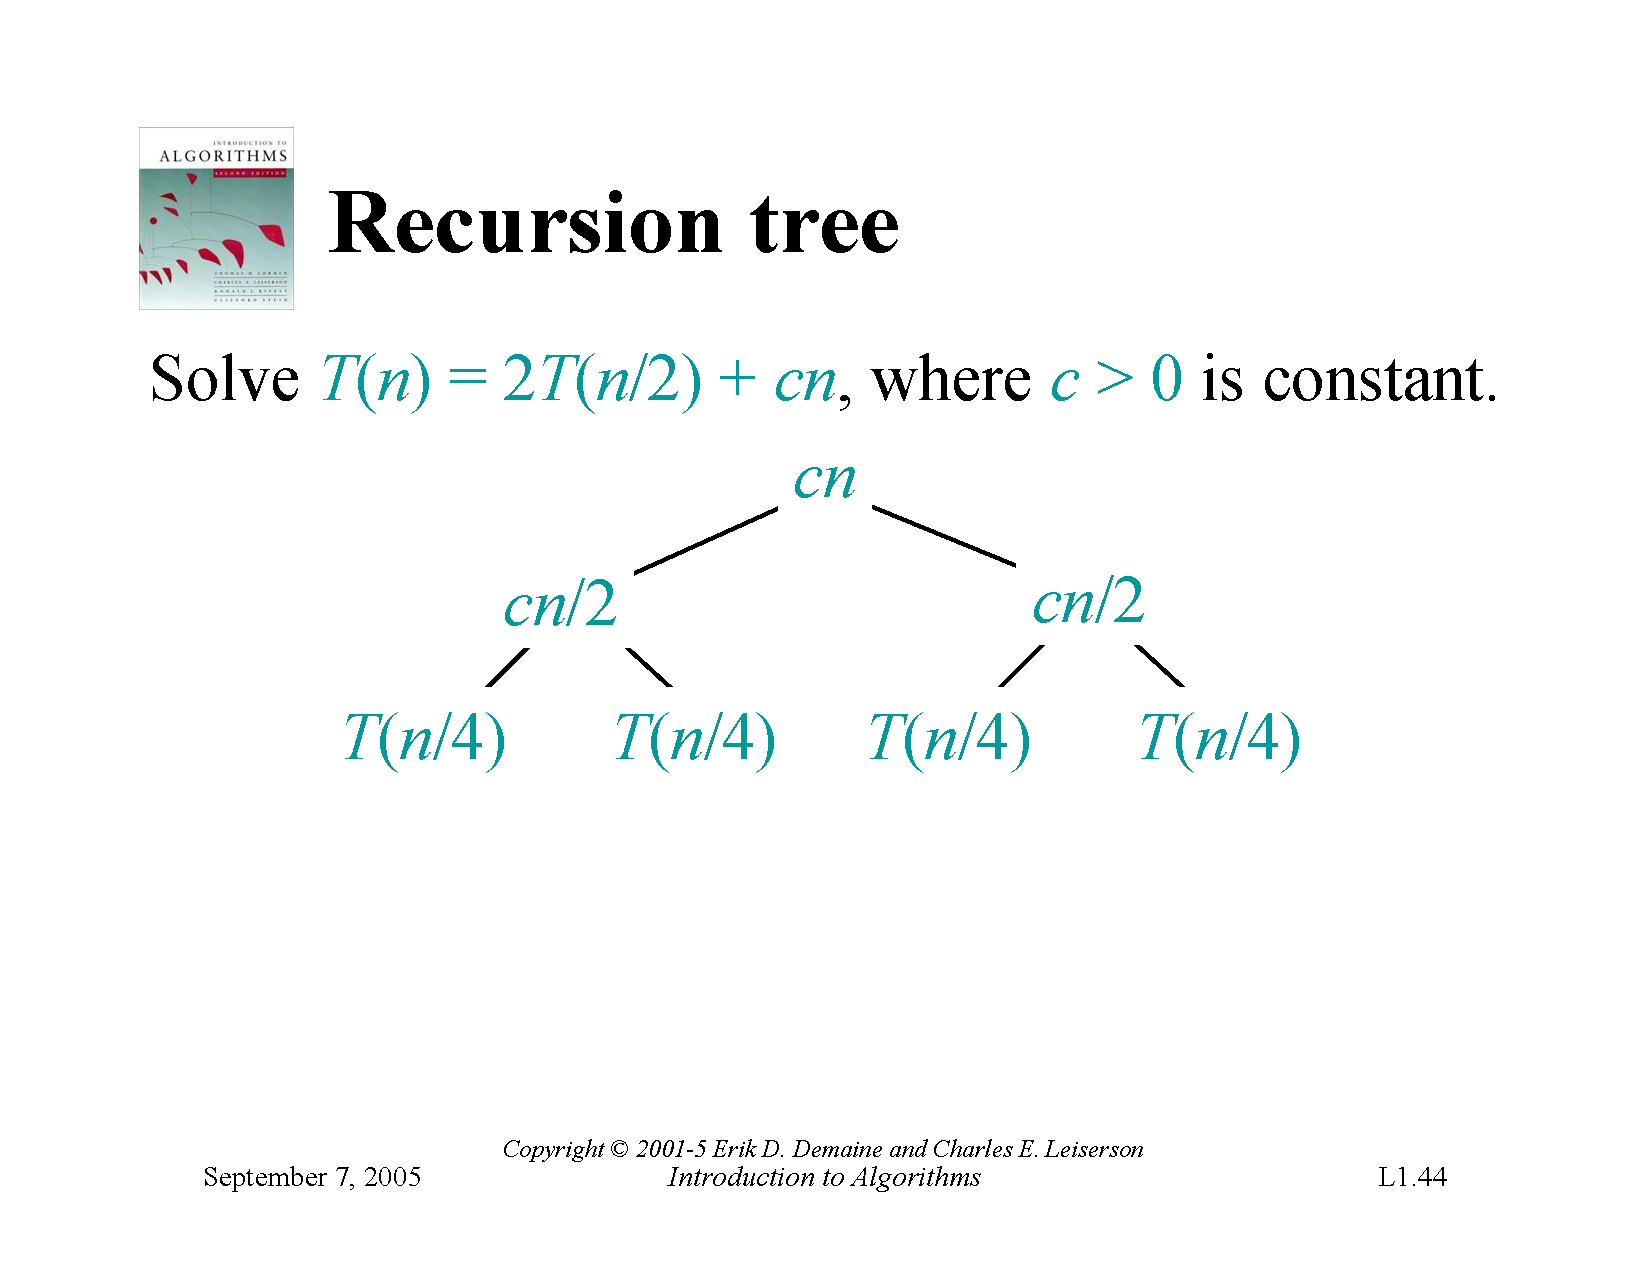
\includegraphics[width=\textwidth, trim={0.49cm 1.25cm 0.7cm 5.75cm}, clip]{pages/lec1_44}
\end{frame}
\begin{frame}{Recursion Tree}
    Solve $T(n) = 2T(\frac{n}{2}) + cn$, where $c > 0$ is constant.\\
    \vspace{5mm}
    \centering
    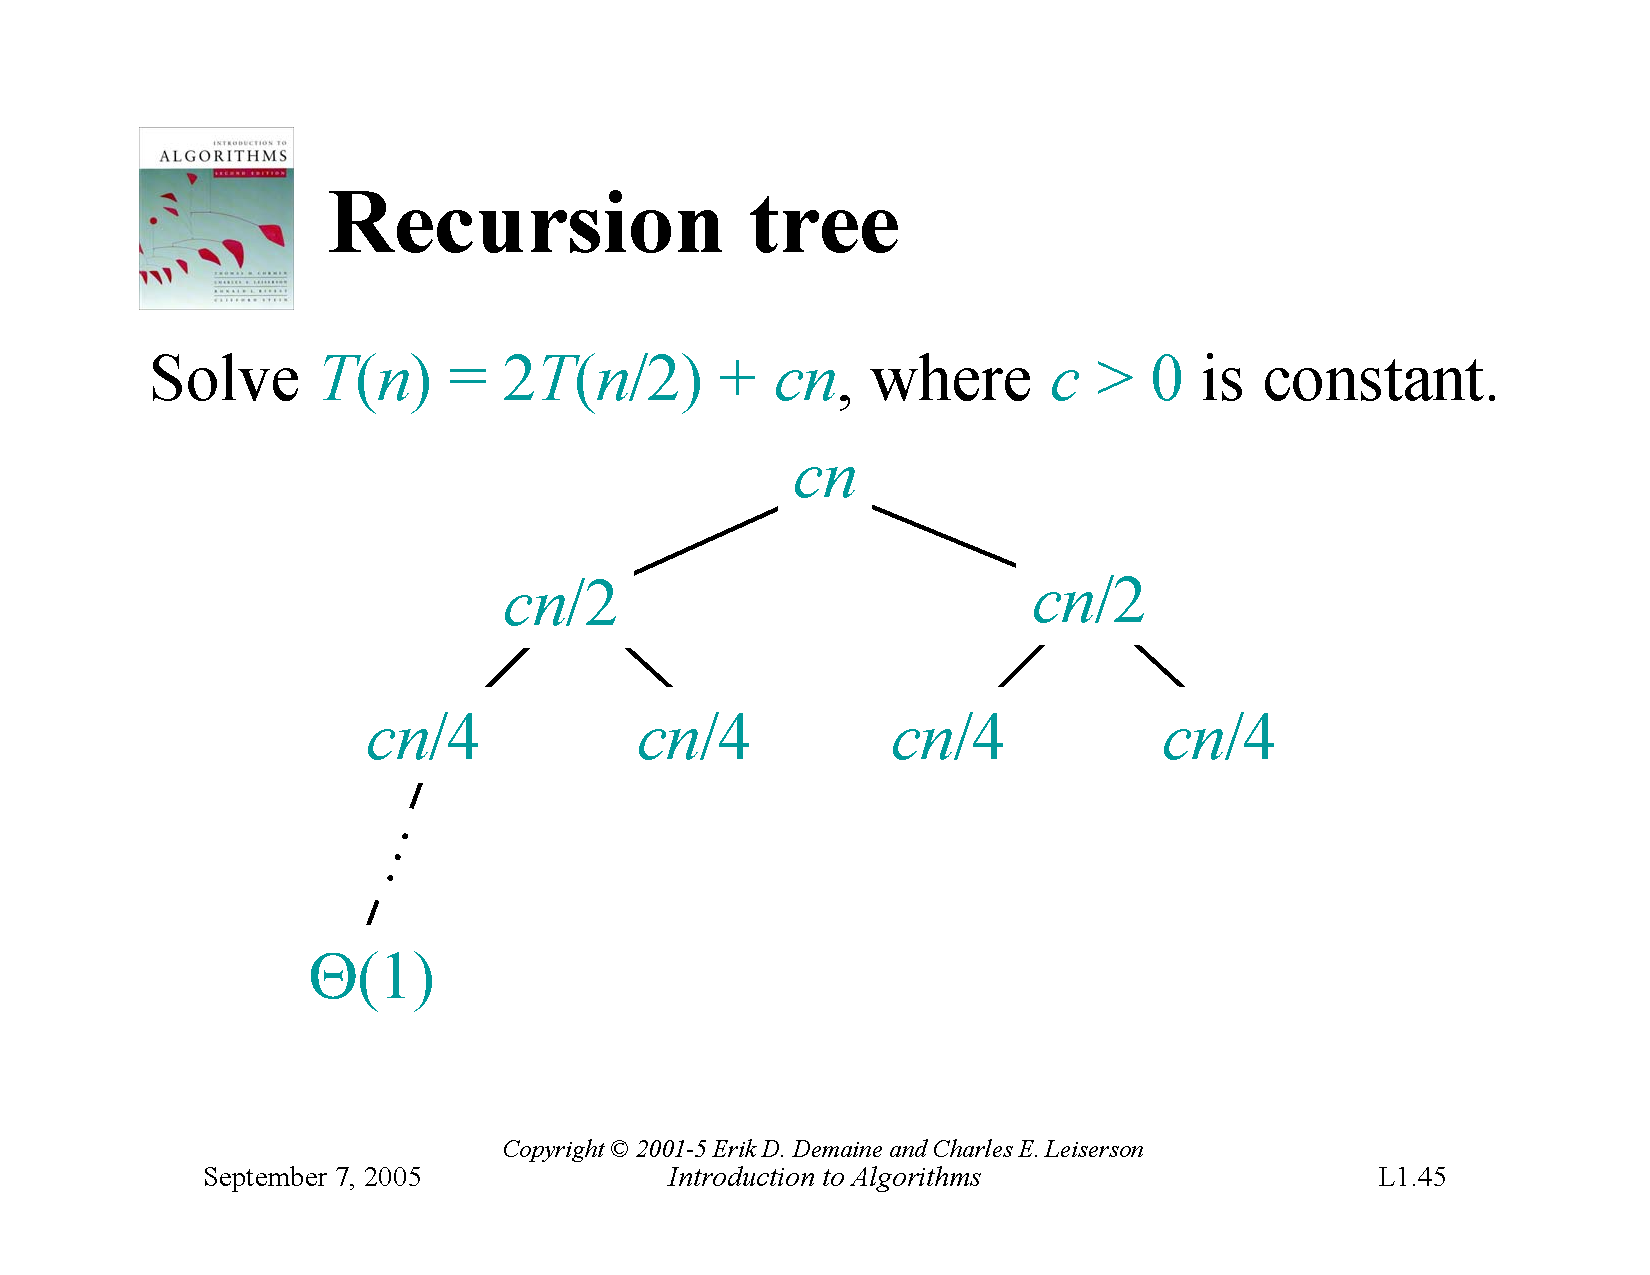
\includegraphics[width=\textwidth, trim={0.49cm 1.25cm 0.7cm 5.75cm}, clip]{pages/lec1_45}
\end{frame}
\begin{frame}{Recursion Tree}
    Solve $T(n) = 2T(\frac{n}{2}) + cn$, where $c > 0$ is constant.\\
    \vspace{5mm}
    \centering
    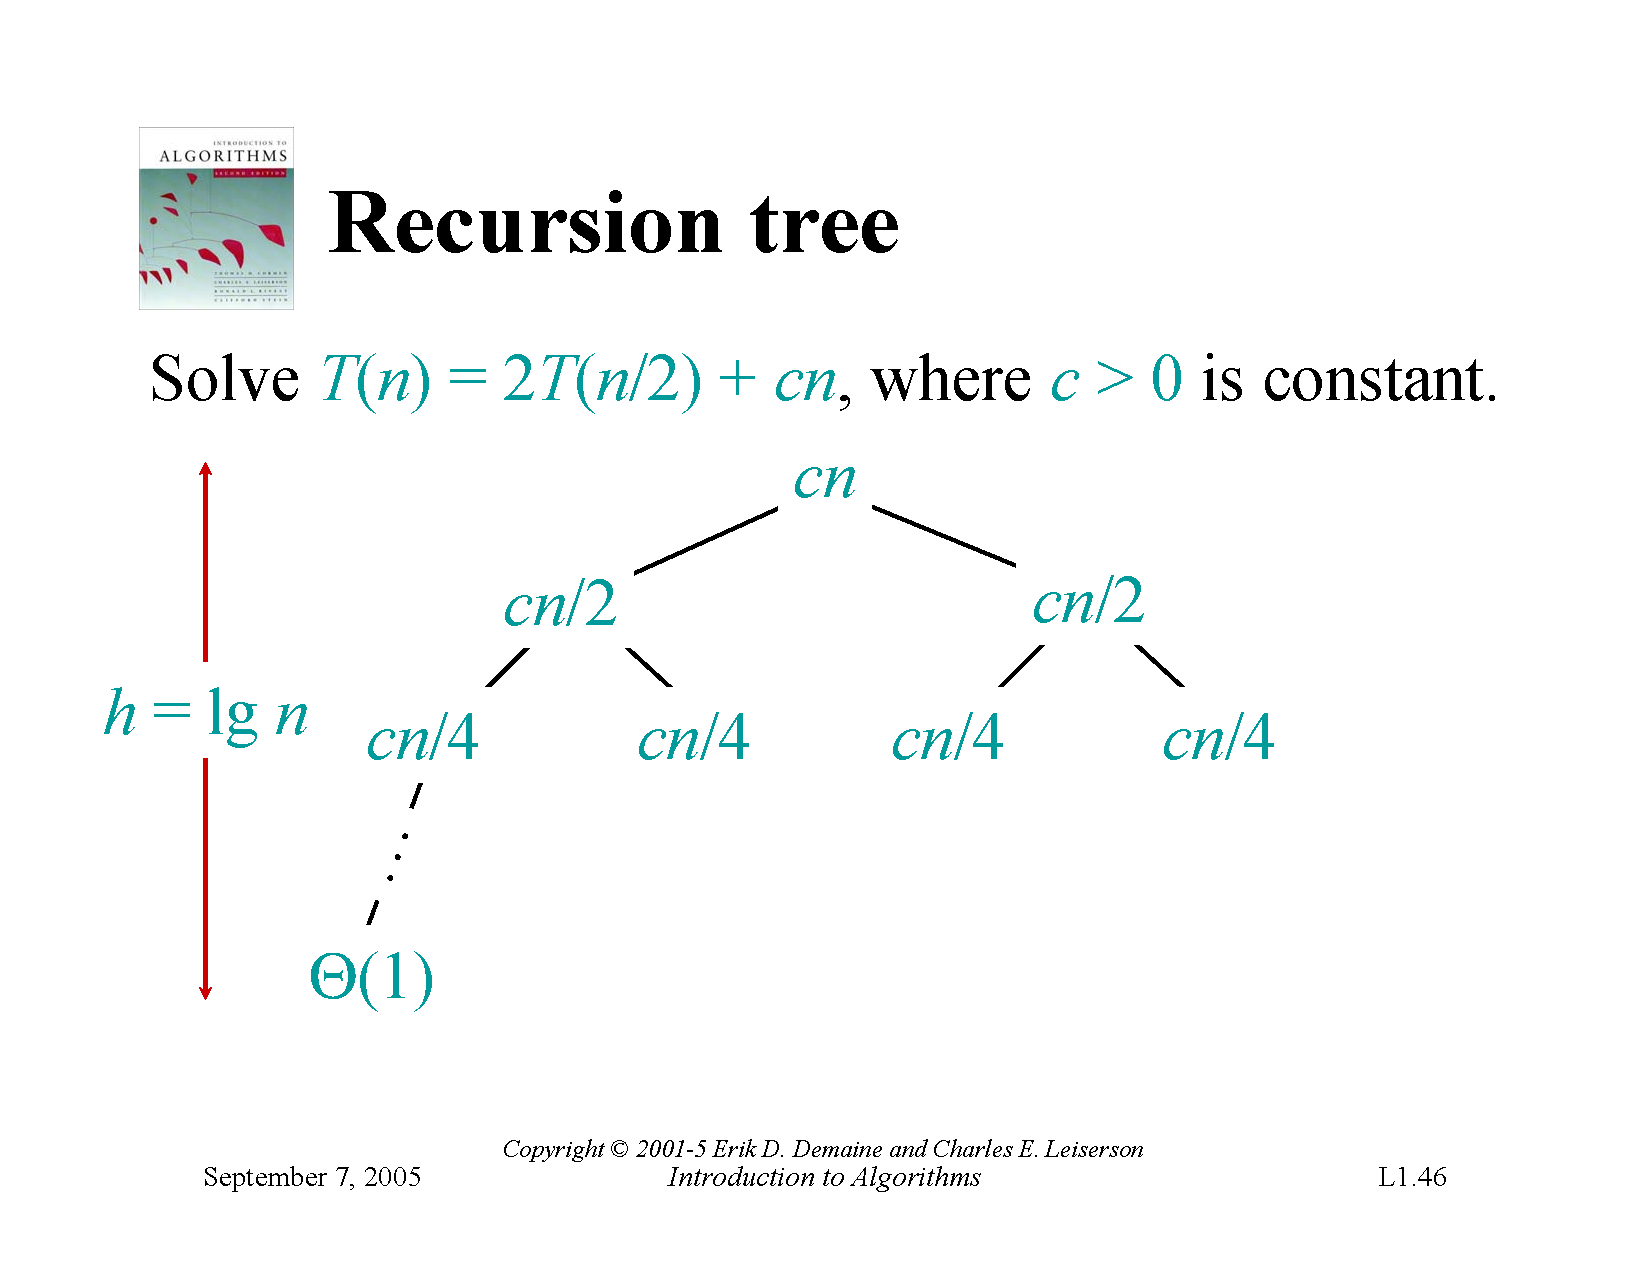
\includegraphics[width=\textwidth, trim={0.49cm 1.25cm 0.7cm 5.75cm}, clip]{pages/lec1_46}
\end{frame}
\begin{frame}{Recursion Tree}
    Solve $T(n) = 2T(\frac{n}{2}) + cn$, where $c > 0$ is constant.\\
    \vspace{5mm}
    \centering
    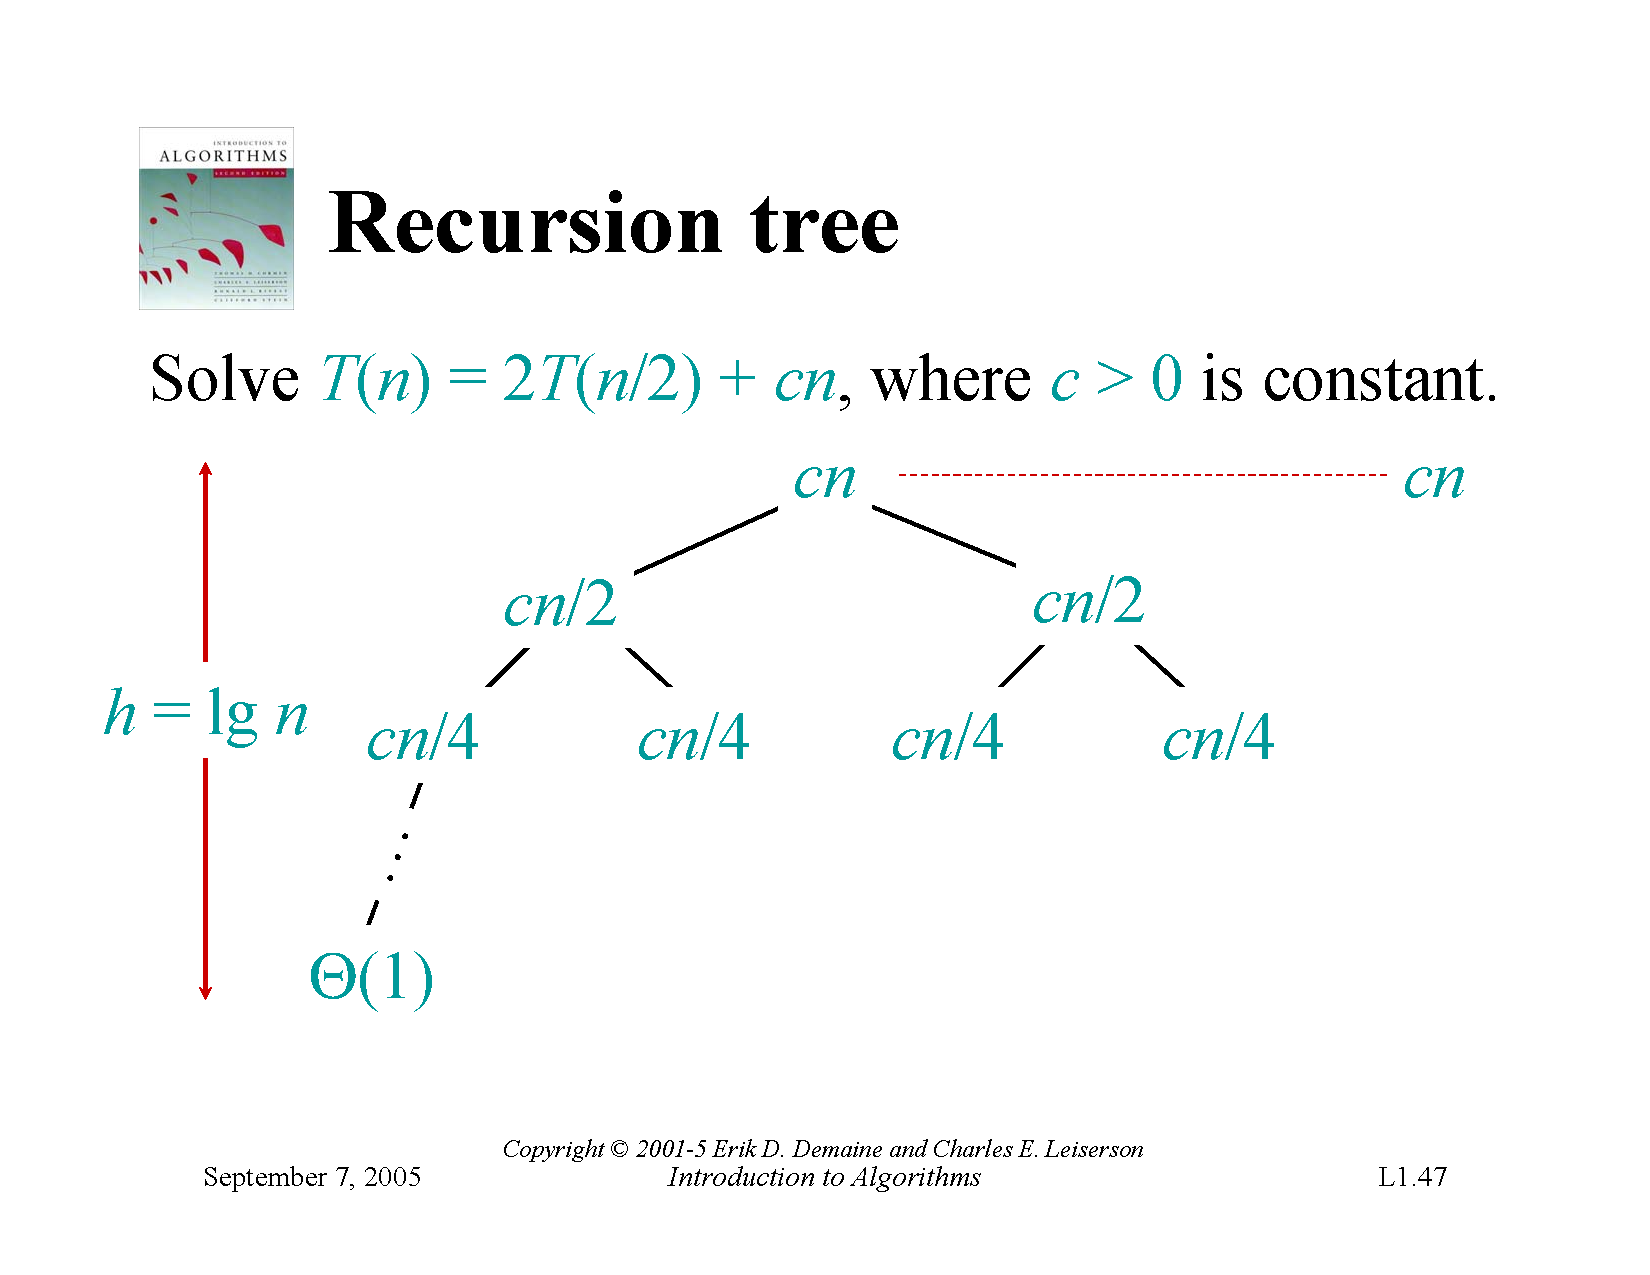
\includegraphics[width=\textwidth, trim={0.49cm 1.25cm 0.7cm 5.75cm}, clip]{pages/lec1_47}
\end{frame}
\begin{frame}{Recursion Tree}
    Solve $T(n) = 2T(\frac{n}{2}) + cn$, where $c > 0$ is constant.\\
    \vspace{5mm}
    \centering
    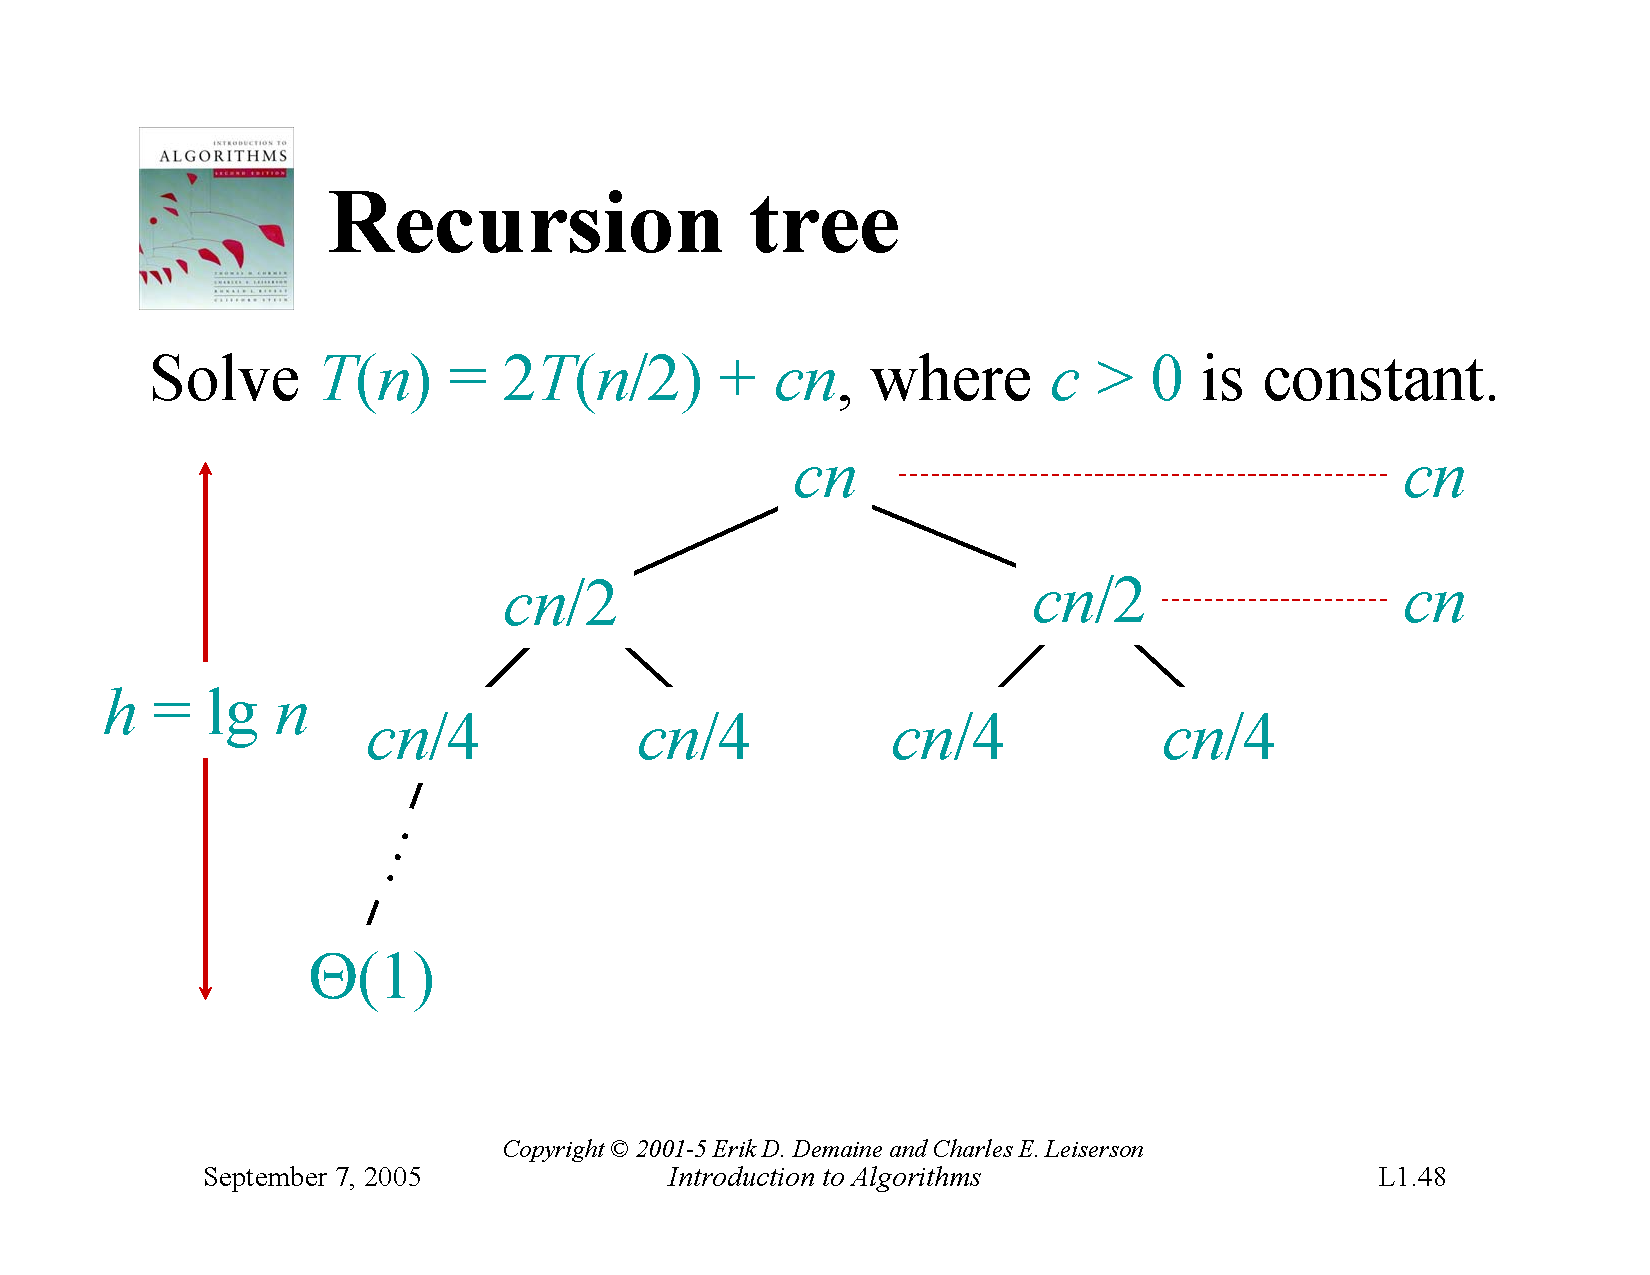
\includegraphics[width=\textwidth, trim={0.49cm 1.25cm 0.7cm 5.75cm}, clip]{pages/lec1_48}
\end{frame}
\begin{frame}{Recursion Tree}
    Solve $T(n) = 2T(\frac{n}{2}) + cn$, where $c > 0$ is constant.\\
    \vspace{5mm}
    \centering
    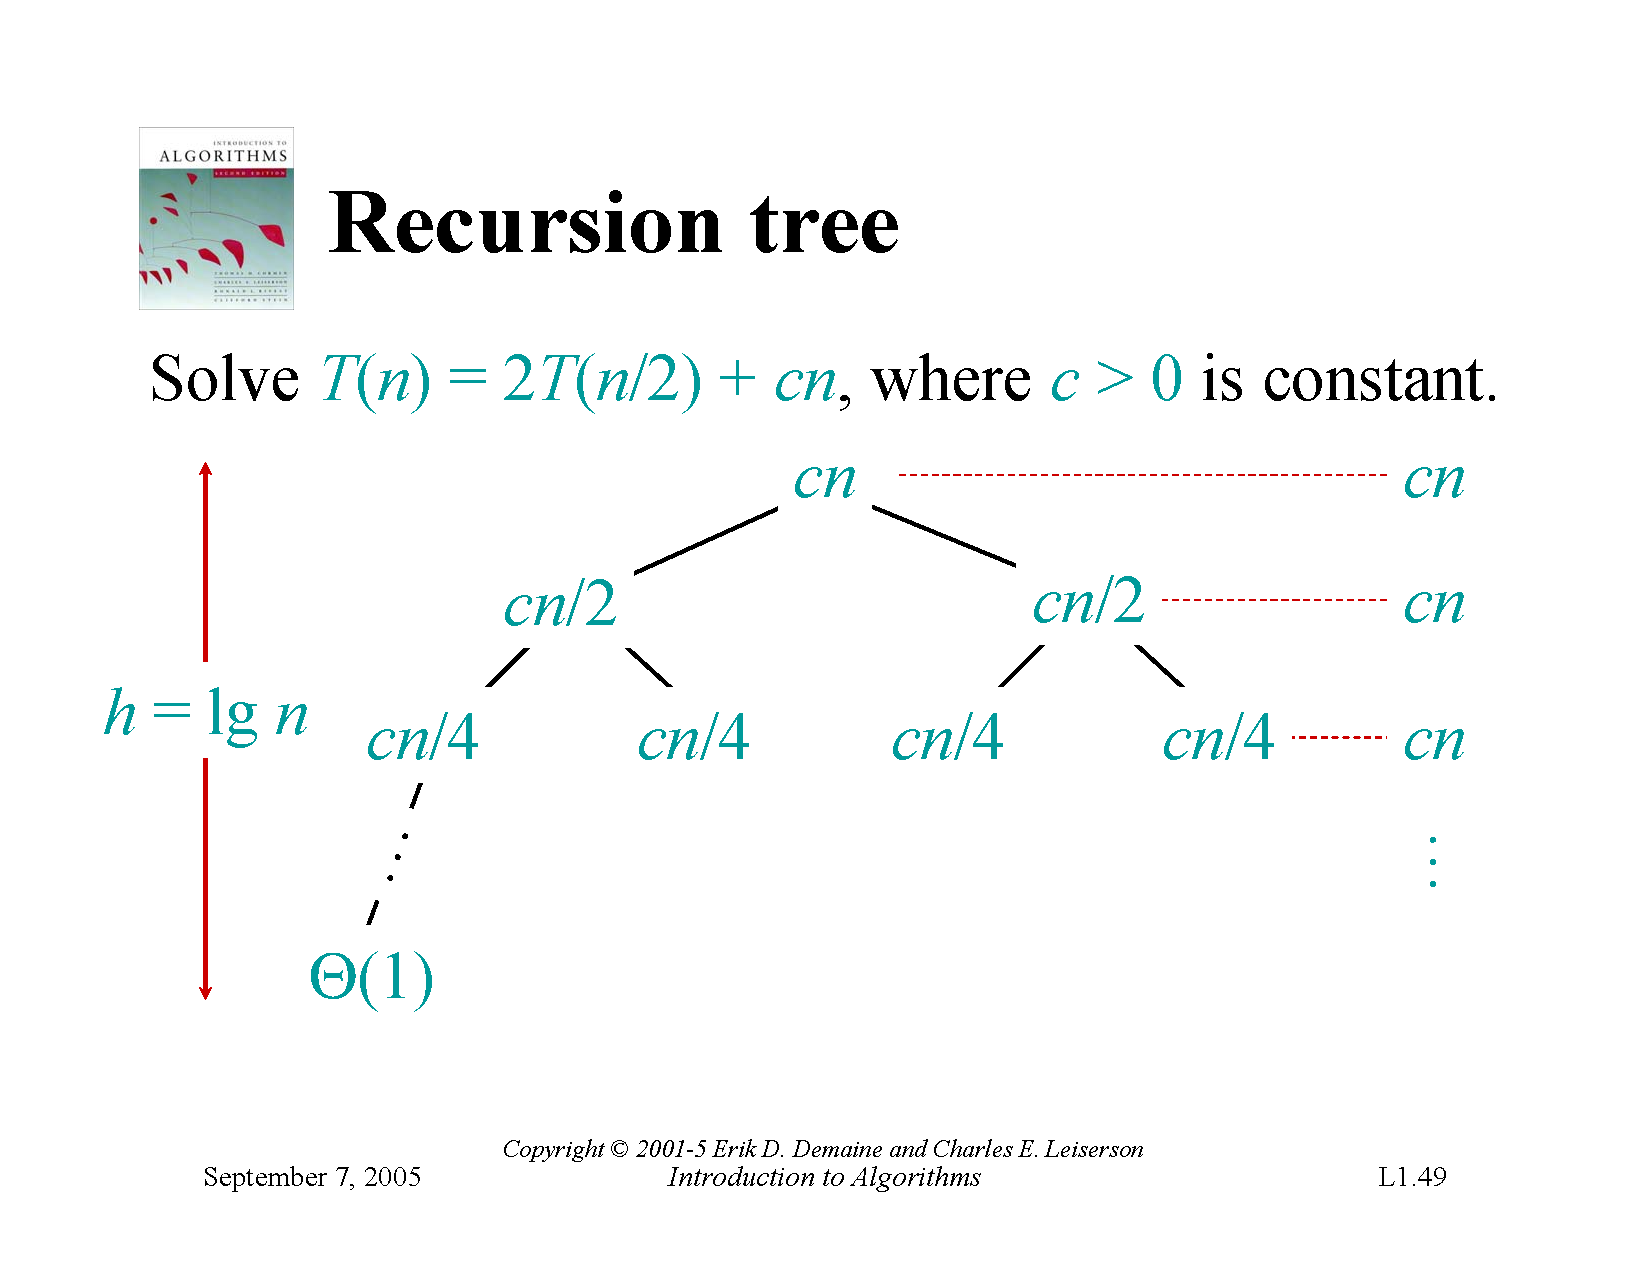
\includegraphics[width=\textwidth, trim={0.49cm 1.25cm 0.7cm 5.75cm}, clip]{pages/lec1_49}
\end{frame}
\begin{frame}{Recursion Tree}
    Solve $T(n) = 2T(\frac{n}{2}) + cn$, where $c > 0$ is constant.\\
    \vspace{5mm}
    \centering
    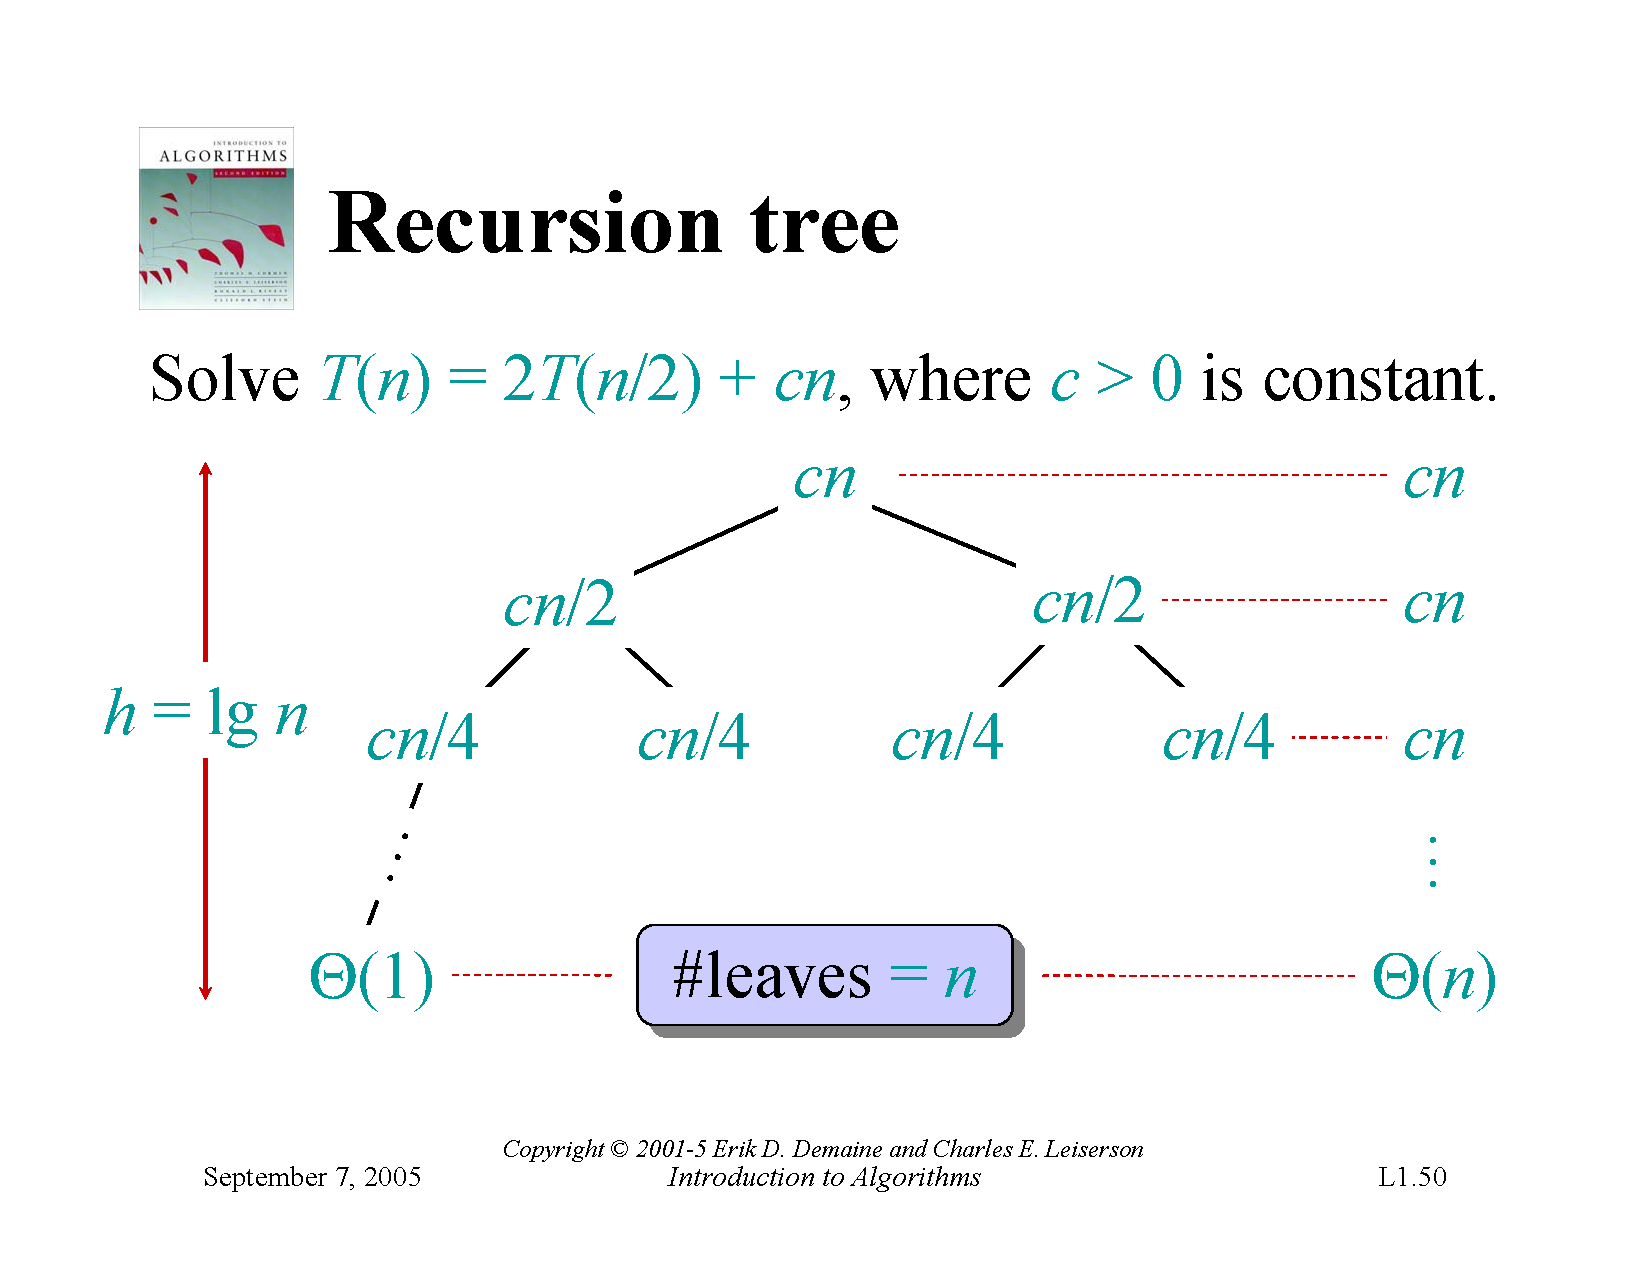
\includegraphics[width=\textwidth, trim={0.49cm 1.25cm 0.7cm 5.75cm}, clip]{pages/lec1_50}
\end{frame}
\begin{frame}{Recursion Tree}
    Solve $T(n) = 2T(\frac{n}{2}) + cn$, where $c > 0$ is constant.\\
    \vspace{5mm}
    \centering
    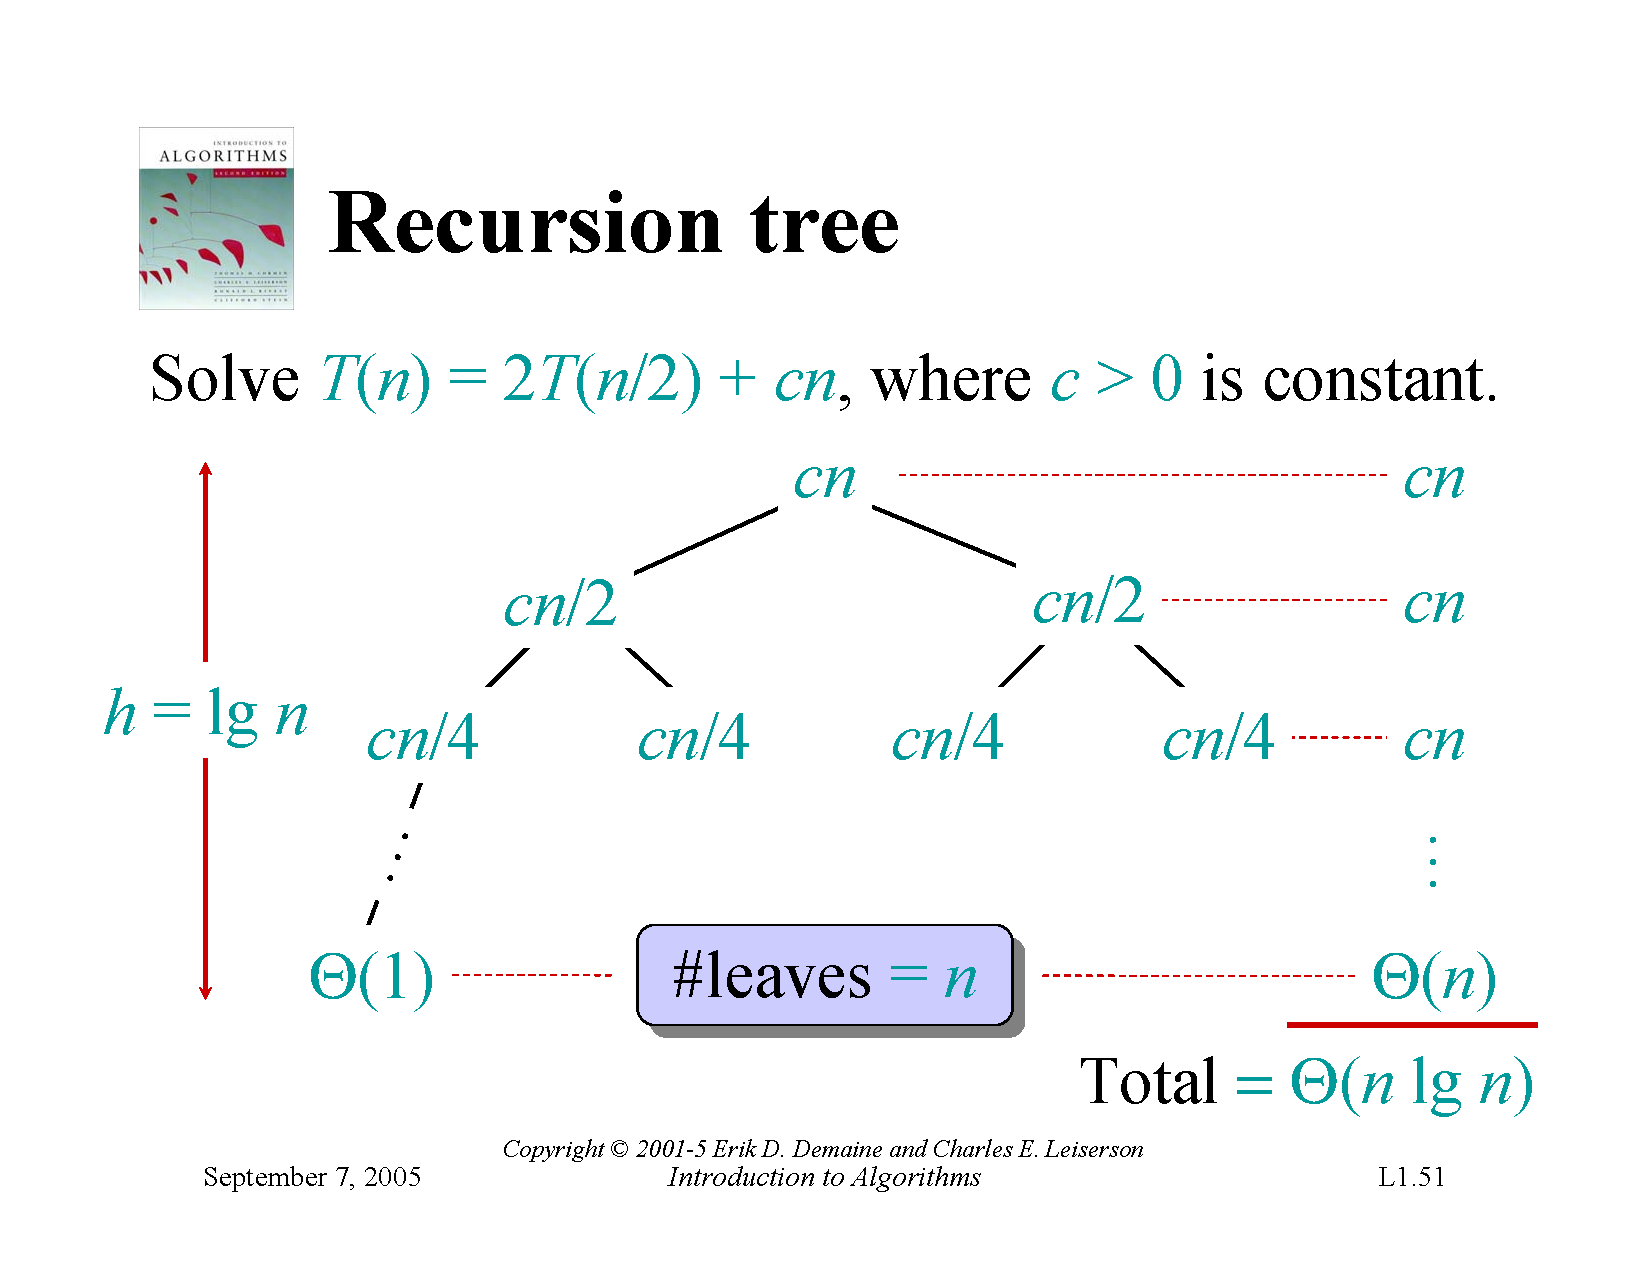
\includegraphics[width=\textwidth, trim={0.49cm 1.25cm 0.7cm 5.75cm}, clip]{pages/lec1_51}
\end{frame}

\section*{Conclusions}

\begin{frame}{Conclusions}
    \begin{itemize}
        \item $\Theta(n log n)$ grows more slowly that $\Theta(n^2)$.
        \item Therefore, merge-sort asymptotically beats insertion-sort in the worst case.
        \item In practice, merge-sort beats insertion-sort for $n > 30$ or so.
        \item Go test it out for yourself!
    \end{itemize}
\end{frame}

\end{document}
